\documentclass[a4paper, 12pt]{report}

\usepackage{
	amsmath,
	amsthm,
	amssymb,
	xcolor,
	soul, 
	cancel, 
	fancyhdr,
	graphicx,
}
\pagestyle{fancy}
\fancyhead[L]{Abstract Algebra}
\fancyhead[R]{\nouppercase{\leftmark}}
\fancyfoot[C]{\thepage}
\usepackage[utf8]{inputenc}
\usepackage[inline]{enumitem}
\usepackage{hyperref}
\hypersetup{
	colorlinks = true,
	linkcolor = black,
}
\usepackage{geometry}
\geometry{
	left = 1in,
	right = 1in,
	top = 1in,
	bottom = 1in,
}
\usepackage[framemethod=tikz]{mdframed}
\usepackage{tikz}

\newcounter{theorem}
\newenvironment{theorem}[1][]{
	\stepcounter{theorem}
	\ifstrempty{#1}{
		\begin{mdframed}[linewidth=1pt,linecolor=blue!10, backgroundcolor=blue!10,]
		\bfseries Theorem~\thechapter.\thetheorem.\normalfont
	}{
		\begin{mdframed}[linewidth=1pt,linecolor=blue!10, backgroundcolor=blue!10,]
		\bfseries Theorem~\thechapter.\thetheorem~(#1).\normalfont
	}
}{\end{mdframed}}
\newenvironment{definition}[1][]{
	\stepcounter{theorem}
	\ifstrempty{#1}{
		\begin{mdframed}[linewidth=1pt, linecolor=gray!15, backgroundcolor=gray!15,]
		\bfseries Definition~\thechapter.\thetheorem.\normalfont
	}{
		\begin{mdframed}[linewidth=1pt, linecolor=gray!15, backgroundcolor=gray!15,]
		\bfseries Definition~\thechapter.\thetheorem~(#1).\normalfont
	}
}{\end{mdframed}}

\newenvironment{proposition}[1][]{
	\stepcounter{theorem}
	\ifstrempty{#1}{
		\begin{mdframed}[linewidth=1pt, linecolor=blue!10, backgroundcolor=blue!10,]
		\bfseries Proposition~\thechapter.\thetheorem.\normalfont
	}{
		\begin{mdframed}[linewidth=1pt, linecolor=blue!10, backgroundcolor=blue!10,]
		\bfseries Proposition~\thechapter.\thetheorem~(#1).\normalfont
	}
}{\end{mdframed}}

\newcounter{corollary}
\newenvironment{corollary}{
	\stepcounter{corollary}
	\begin{mdframed}[linecolor=blue!10, backgroundcolor=blue!10, linewidth=1pt,]
	\bfseries Corollary~\thechapter.\thecorollary.\normalfont
}{\end{mdframed}}

\newenvironment{lemma}[1][]{
	\stepcounter{theorem}
	\ifstrempty{#1}{
		\begin{mdframed}[linewidth=1pt, linecolor=yellow!30, backgroundcolor=yellow!30,]
		\bfseries Lemma~\thechapter.\thetheorem.\normalfont
	}{
		\begin{mdframed}[linewidth=1pt, linecolor=yellow!30, backgroundcolor=yellow!30,]
		\bfseries Lemma~\thechapter.\thetheorem~(#1).\normalfont
	}
}{\end{mdframed}}

\newenvironment{example}[1][]{
	\ifstrempty{#1}{
		\begin{mdframed}[linewidth=1pt, linecolor=red!10, backgroundcolor=red!20,]
		\bfseries Example.\normalfont
	}{
		\begin{mdframed}[linewidth=1pt, linecolor=red!10, backgroundcolor=red!20,]
		\bfseries Example~(#1).\normalfont
	}
}{\end{mdframed}}

\newenvironment{exercise}{
	\begin{mdframed}[linewidth=1pt, linecolor=green!10, backgroundcolor=green!10,]
	\bfseries Exercise.\normalfont
}{\end{mdframed}}

\title{
	{Abstract Algebra}\\
	\small Reading Project: Summer of Science\\
	Indian Institute of Technology Bombay\\
	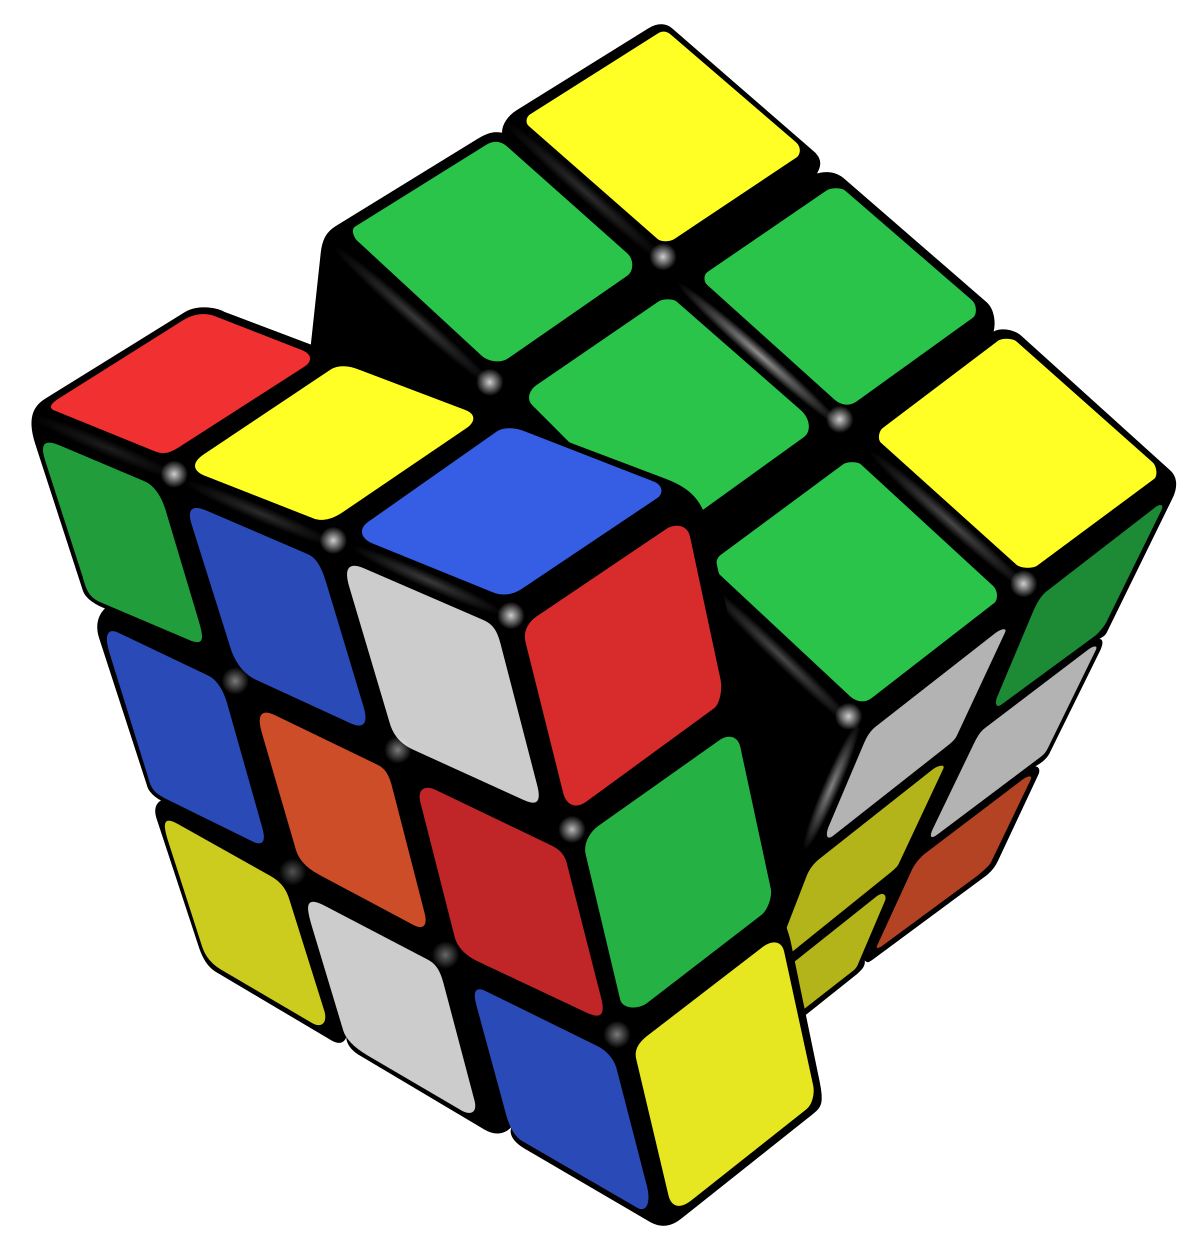
\includegraphics[width=0.5\textwidth]{../images/grouptheory.png}
}
\author{Swayam Chube\\\textbf{Mentor:} Shourya Pandey}
\date{Date of Submission : \today}

\renewcommand{\qedsymbol}{$\blacksquare$}
\newcommand{\N}{\mathbb{N}}
\newcommand{\Z}{\mathbb{Z}}
\newcommand{\Q}{\mathbb{Q}}
\newcommand{\R}{\mathbb{R}}
\newcommand{\F}{\mathbb{F}}
\newcommand{\Pb}{\mathbb{P}}
\newcommand{\vphi}{\varphi}
\newcommand{\aut}{\operatorname{Aut}}
\newcommand{\inn}{\operatorname{Inn}}
\newcommand{\stab}{\operatorname{stab}}
\newcommand{\orb}{\operatorname{orb}}
\newcommand{\lcm}{\operatorname{lcm}}
\newcommand{\vtri}{\vartriangleleft}
\newcommand{\Ker}{\operatorname{Ker}}
\newcommand{\chr}{\operatorname{char}}
\newcommand{\cl}{\operatorname{cl}}
\newcommand{\Cay}{\operatorname{Cay}}
\newcommand{\wt}{\operatorname{wt}}
\newcommand{\Gal}{\operatorname{Gal}}

\setcounter{chapter}{0}
\setlength{\parindent}{0pt}
\begin{document}
	\maketitle
	\tableofcontents

\chapter*{Introduction}
	This is the report for the Summer of Science Reading Project for Abstract Algebra under the mentorship of Shourya Pandey. The reference text used for preparing the same was \textbf{Contemporary Abstract Algebra by Joseph A. Gallian}. \\
	
	It is known to me that this report is notably long which is partly due to me getting carried away with the details of proofs during the first half of the project. In order to keep the reader engaged in the text, I have decided to omit long and routine proofs in the latter half of the report, but the theorems have still been cited in full detail. \\
	
	The most important parts are Parts I, II and III which deal with Groups, Rings and Fields respectively. Part IV which deals with special topics has not been talked about in exceeding detail in order to refrain from making this report too technical and lackluster.

\part{Groups}
	\chapter{An Introduction To Groups}
	We shall have a look at groups from the point of view of symmetry operations and then formalize the definition for abstract operations.\\
Say we want to study the symmetry elements of a planar equilateral triangle. First let us label the vertices of the traingle as $A$, $B$ and $C$. Studying the symmetry operations is almost like studying the permissible permutations of $A$, $B$ and $C$ around the vertices of the given triangle. Pictorially, we can have the following symmetry operations:\\
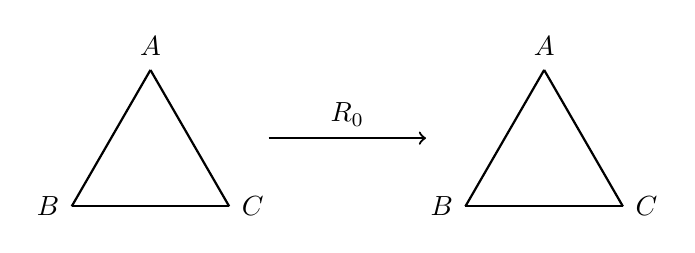
\begin{tikzpicture}
	\draw (1,2.032) node{$A$};
	\draw (-0.3,0) node{$B$};
	\draw (2.3,0) node{$C$};
	\draw (6,2.032) node{$A$};
	\draw (4.7,0) node{$B$};
	\draw (7.3,0) node{$C$};
	\draw (3.5,1.166) node{$R_0$};
	\draw[thick](0,0)--(1,1.732); 
	\draw[thick](0,0)--(2,0);
	\draw[thick](1,1.732)--(2,0);
	\draw[thick,->](2.5,0.866)--(4.5,0.866);
	\draw[thick](5,0)--(6,1.732);
	\draw[thick](5,0)--(7,0);
	\draw[thick](6,1.732)--(7,0);
\end{tikzpicture}
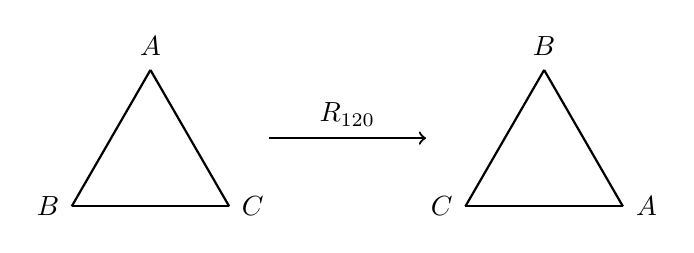
\begin{tikzpicture}
	\draw (1,2.032) node{$A$};
	\draw (-0.3,0) node{$B$};
	\draw (2.3,0) node{$C$};
	\draw (6,2.032) node{$B$};
	\draw (4.7,0) node{$C$};
	\draw (7.3,0) node{$A$};
	\draw (3.5,1.166) node{$R_{120}$};
	\draw[thick](0,0)--(1,1.732); 
	\draw[thick](0,0)--(2,0);
	\draw[thick](1,1.732)--(2,0);
	\draw[thick,->](2.5,0.866)--(4.5,0.866);
	\draw[thick](5,0)--(6,1.732);
	\draw[thick](5,0)--(7,0);
	\draw[thick](6,1.732)--(7,0);
\end{tikzpicture}
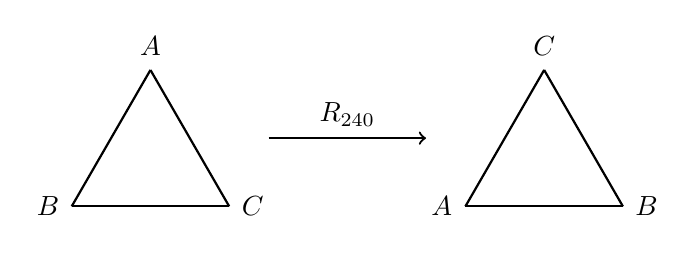
\begin{tikzpicture}
	\draw (1,2.032) node{$A$};
	\draw (-0.3,0) node{$B$};
	\draw (2.3,0) node{$C$};
	\draw (6,2.032) node{$C$};
	\draw (4.7,0) node{$A$};
	\draw (7.3,0) node{$B$};
	\draw (3.5,1.166) node{$R_{240}$};
	\draw[thick](0,0)--(1,1.732); 
	\draw[thick](0,0)--(2,0);
	\draw[thick](1,1.732)--(2,0);
	\draw[thick,->](2.5,0.866)--(4.5,0.866);
	\draw[thick](5,0)--(6,1.732);
	\draw[thick](5,0)--(7,0);
	\draw[thick](6,1.732)--(7,0);
\end{tikzpicture}
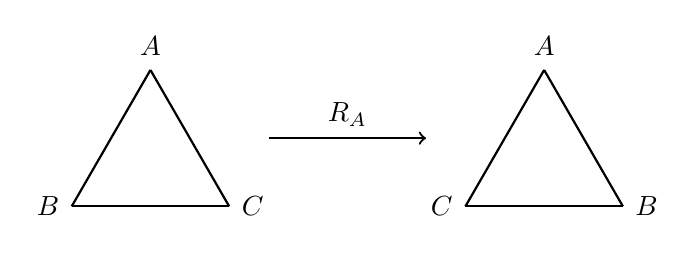
\begin{tikzpicture}
	\draw (1,2.032) node{$A$};
	\draw (-0.3,0) node{$B$};
	\draw (2.3,0) node{$C$};
	\draw (6,2.032) node{$A$};
	\draw (4.7,0) node{$C$};
	\draw (7.3,0) node{$B$};
	\draw (3.5,1.166) node{$R_A$};
	\draw[thick](0,0)--(1,1.732); 
	\draw[thick](0,0)--(2,0);
	\draw[thick](1,1.732)--(2,0);
	\draw[thick,->](2.5,0.866)--(4.5,0.866);
	\draw[thick](5,0)--(6,1.732);
	\draw[thick](5,0)--(7,0);
	\draw[thick](6,1.732)--(7,0);
\end{tikzpicture}
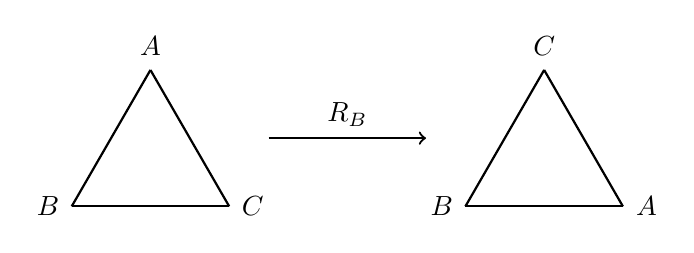
\begin{tikzpicture}
	\draw (1,2.032) node{$A$};
	\draw (-0.3,0) node{$B$};
	\draw (2.3,0) node{$C$};
	\draw (6,2.032) node{$C$};
	\draw (4.7,0) node{$B$};
	\draw (7.3,0) node{$A$};
	\draw (3.5,1.166) node{$R_B$};
	\draw[thick](0,0)--(1,1.732); 
	\draw[thick](0,0)--(2,0);
	\draw[thick](1,1.732)--(2,0);
	\draw[thick,->](2.5,0.866)--(4.5,0.866);
	\draw[thick](5,0)--(6,1.732);
	\draw[thick](5,0)--(7,0);
	\draw[thick](6,1.732)--(7,0);
\end{tikzpicture}
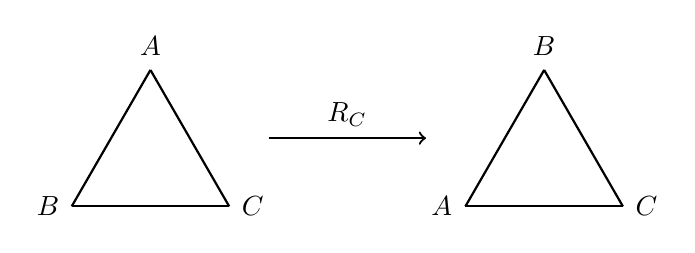
\begin{tikzpicture}
	\draw (1,2.032) node{$A$};
	\draw (-0.3,0) node{$B$};
	\draw (2.3,0) node{$C$};
	\draw (6,2.032) node{$B$};
	\draw (4.7,0) node{$A$};
	\draw (7.3,0) node{$C$};
	\draw (3.5,1.166) node{$R_C$};
	\draw[thick](0,0)--(1,1.732); 
	\draw[thick](0,0)--(2,0);
	\draw[thick](1,1.732)--(2,0);
	\draw[thick,->](2.5,0.866)--(4.5,0.866);
	\draw[thick](5,0)--(6,1.732);
	\draw[thick](5,0)--(7,0);
	\draw[thick](6,1.732)--(7,0);
\end{tikzpicture}
Where $R_\theta$ denotes a clockwise rotation about the center of the triangle by $\theta$ degrees while $R_A$ denotes the reflection through the plane of symmetry passing through $A$ which (obviously) is perpendicular to $\overline{BC}$.\\
So, in total, we have six symmetry elements for a planar equilateral triangle. Let us now study the composition of these symmetry elements.\\
Obviously $R_0$ composed with any symmetry element $\mathcal{S}$ should result in $\mathcal{S}$ and $R_\theta$ composed with $R_\alpha$ would result in $R_{\theta+\alpha}$. But $R_A\circ R_{120}$ results in $R_C$ whereas $R_{120}\circ R_A$ results in $R_B$. Representing all these in a tabular form, we obtain what is known as the Cayley table or more colloquially, a multiplication/operation table.\\
Note that for the table, the composition order is $(\text{column}\circ\text{row})$.
\begin{center}
\begin{tabular}{c|c c c c c c}
	  & $R_{0}$ & $R_{120}$ & $R_{240}$ & $R_{A}$ & $R_{B}$ & $R_{C}$\\
	  \hline
	  $R_0$ & $R_{0}$ & $R_{120}$ & $R_{240}$ & $R_{A}$ & $R_{B}$ & $R_{C}$\\
	  $R_{120}$ & $R_{120}$ & $R_{240}$ & $R_{0}$ & $R_C$ & $R_A$ & $R_B$\\
	  $R_{240}$ & $R_{240}$ & $R_0$ & $R_{120}$ & $R_B$ & $R_C$ & $R_A$\\
	  $R_A$ & $R_A$ & $R_B$ & $R_C$ & $R_0$ & $R_{120}$ & $R_{240}$\\
	  $R_B$ & $R_B$ & $R_C$ & $R_A$ & $R_{240}$ & $R_0$ & $R_{120}$\\
	  $R_C$ & $R_C$ & $R_A$ & $R_B$ & $R_{120}$ & $R_{240}$ & $R_0$\\
\end{tabular}
\end{center}

The above table shows us that the composition of any two symmetry elements gives another symmetry element. This property is called \textit{closure} which is a necessary property for a group. Also, note that $a\circ b$ need not be the same as $b\circ a$. But, in the case when $a\circ b=b\circ a$ for all elements $a$ and $b$, the group is said to be \textit{commutative} or a scarier term for the same is \textit{Abelian}\footnote{Named after Neils Henrik Abel}. Finally, one can check that $(a\circ b)\circ c=a\circ(b\circ c)$ for any three symmetry elements $a$, $b$ and $c$.\footnote{I shall leave the verification of this as an exercise for the reader} This property is called \textit{associativity} which is another necessary property for a group.\\

From the above discussion, we can conclude that the set of symmetries of a planar equilateral triangle forms a group.\footnote{This is a slight abuse of language, since a group needs a binary operator associated with it but we shall deal with this in the next chapter.} This group is denoted by $D_3$ and is called ``the dihedral group of order $6$". Note that the order of the group is determined by the number of elements. In general, $D_n$ is used to represent the set of symmetries of a planar $n$-gon. A natural question to ask at this point is whether the order of $D_n$ is $2n$ (which you may or may not have conjectured while dealing with $D_3$).\\
The answer is \textbf{yes}. It is rather easy to prove. Let us consider a general $n$-gon given by $A_1A_2\cdots A_n$. We are interested in the ``permissible permutations" of $A_1A_2\cdots A_n$. We note that any symmetry does not change the ``adjacency" of the vertices that is, in particular, $A_1$ and $A_2$ must be adjacent in all such permutations. Now, for all the permutations, $A_1$ can be placed in $n$ positions. Once the position of $A_1$ has been decided, there are only two valid placements of $A_2$. Once the positions of both $A_1$ and $A_2$ have been decided, the positions of all the vertices get determined. Thus, only $n\times2=2n$ symmetry elements are possible.





	
	\chapter{Formalizing Groups}
	In the previous chapter, we tried to develop the notion of a group in an informal way. In this chapter, we would like to formalize that same notion. For this, we begin with the definition of a binary operation
\begin{definition}[Binary Operation]
	Let $G$ be a set. A binary operation $\circ$ is simply a function~$\circ:G\times G\to G$ 
\end{definition}

Equipped with the above definition, we are now ready to define a group
\begin{definition}
	Let $G$ be a set and $\circ$ be a binary operation on $G$, then the ordered pair $(G,\circ)$ is said to be a group if the following conditions are satisfied:
	\begin{enumerate}
		\item\textit{Associativity.} For any three (not necessarily distinct) elements $a,b,c\in G$, $a\circ(b\circ c)=(a\circ b)\circ c$.
		\item\textit{Identity.} There exists an element $e$ in $G$ such that $a\circ e=a=e\circ a$ for all elements $a\in G$.
		\item\textit{Inverses.} For all elements $a\in G$, there exists $b\in G$ such that $a\circ b=e=b\circ a$.
	\end{enumerate}
\end{definition}

By the way, note that the definition of a binary operation itself implies that the group is closed, so we need not provide a separate axiom for \textit{closure}.\\

\textbf{Examples of Groups}
\begin{enumerate}
	\item $(\Z,+)$, $(\R,+)$, $(\Q,+)$
	\item $(\R\backslash\{0\},\times)$ and $(\Q\backslash\{0\},\times)$
	\item $(D_n,\circ)$ where $\circ$ is the binary operator for composition of symmetries.
	\item $(GL(n,\R),\times)$ where $GL(n,\R)$ is the set of invertible square matrices of order $n$ with real entries and $\times$ is matrix multiplication. This group is called the \textit{general linear group} of $n\times n$ matrices over $\R$.
\end{enumerate}

\textbf{Examples of non-Groups}
\begin{enumerate}
	\item $(\N,+)$. Since there is no identity in $\N$.
	\item $(\R,\times)$ and $(\Q,\times)$. Since $0$ does not have an inverse.
\end{enumerate}

\begin{exercise}
	Let $U(n)$ denote the set of all natural numbers, less than or equal to $n$ which are coprime to $n$. Show that $(U(n),\cdot)$ where $\cdot$ is multiplication modulo $n$ forms a group.
\end{exercise}
\begin{proof}
	Verifying closure is trivial. Further, it is easy to verify that $1\in U(n)$ is the required identity. Finally, we are left with proving the existance of inverses. Let $a\in U(n)$. Recall, from Bezout's Lemma, there must exist integers $x$ and $y$ such that 
	$$
	ax+ny=\gcd(a,n) = 1
	$$
	Reducing the above equation modulo $n$, we obtain (for some $x'>0$)
	$$
	ax'\equiv1\pmod n
	$$
	The above equation also implies that $\gcd(x',n)=1$, and thus $x'\in U(n)$ and is an inverse of $a$. Since $(U(n),\cdot)$ satisfies the group axioms, it is indeed a group. Further, since multiplication is commutative modulo $n$, the group is also \textit{Abelian}.
\end{proof}


Now that we have seen sufficient examples of groups, we shall have a look at some general properties of groups.\\

Here onwards, for some binary operation $\circ$, $a\circ b$ shall be represented simply by $ab$.

\begin{proposition}[Uniqueness of Identity]
	Let $(G,\circ)$ be a group. Then the identity element of the group is unique.
\end{proposition}
\begin{proof}
	Since $(G,\circ)$ is known to be a group, it has atleast one identity. Suppose, there exist two identies $e_1$ and $e_2$. Then, according to the definition of the identity,
	$$
	e_1 = e_1e_2 = e_2e_1 = e_2
	$$
	This implies that the identity is unique.
\end{proof}
\begin{proposition}[Left and Right Cancellation]
	Let $(G,\circ)$ be a group. Let $a,b,c\in G$.
	\begin{itemize}
		\item If $ba=ca$, then $b=c$
		\item If $ab=ac$, then $b=c$
	\end{itemize}
\end{proposition}
\begin{proof}
	Proving one of them is sufficient, since the proof of the other follows similarly. We have 
	$$
	ba = ca \Longrightarrow  \underbrace{(ba)a^{-1} =(ca)a^{-1} \Longrightarrow b(aa^{-1})=c(aa^{-1})}_{\text{due to associativity}} \Longrightarrow b=c
	$$
\end{proof}
\begin{proposition}[Uniqueness of Inverse]
	Let $(G,\circ)$ be a group. For every $a\in G$, there exists a unique inverse $b\in G$ for the aforementioned $a$.
\end{proposition}
\begin{proof}
	Since $G$ is known to be a group, $a$ has atleast one inverse. Suppose there exist two inverses $b$ and $c$ for $a$. Then, 
	$$
	b = be = b(ac) = (ba)c = c
	$$
	This implies that the inverse of $a$ is unique.
\end{proof}

\begin{proposition}
	Let $a,b\in G$. Then $(ab)^{-1}=b^{-1}a^{-1}$
\end{proposition}
\begin{proof}
	Note that 
	$$
	e = aa^{-1} = (ae)a = (a(bb^{-1}))a^{-1} = ((ab)b^{-1})a^{-1} = (ab)(b^{-1}a^{-1})
	$$
	and due to the uniqueness of the inverse, we have the desired conclusion.
\end{proof}








	
	\chapter{Finite Groups and Subgroups}
	We briefly talked about the orders of goups in \textbf{Chapter 1}, putting that formally, we have 
\begin{definition}[Order of a Group]
	Let $(G,\circ)$ be a group. If $G$ has a finite number of elements, then we say the order of $G$, denoted by $|G|$ is equal to the number of elements. If $G$ is not finite, then we say that the order of $G$ is infinite.
\end{definition}

Just as we define the order of a group, we can define the order of an element in a group.
\begin{definition}[Order of an Element]
	Let $(G,\circ)$ be a group. Let $g\in G$. The order of $g$ is defined to be the smallest posistive integer satisfying $g^n=e$ where $e$ is the identity element in $G$. If no such $n$ exists, then $g$ is said to have infinite order. The order of $g$ is denoted by $|g|$.
\end{definition}

\begin{proposition}
	Let $(G,\circ)$ be a finite group. Then, for every element $g\in G$, $|g|$ is finite.
\end{proposition}
\begin{proof}
	Consider the set 
	$$
	\{g,g^2,\cdots,g^{|G|+1}\}
	$$
	Since $G$ is closed under $\circ$, the above set must be a subset of $G$ but due to the Pigeon-hole Principle, there must exist two distinct indices $i>j$ such that $g^i=g^j$. This implies that $g^{(i-j)}=e$, implying that the order of $g$ is $i-j\le n$ which is obviously finite.
\end{proof}

\begin{definition}[Subgroup]
	Let $(G,\circ)$ be a group. If $H\subseteq G$ and $(H,\circ)$ forms a group, then $H$ is said to be a subgroup of $G$.
\end{definition}

In what follows, we shall discuss three propositions which are useful for determining whether or not a group is a subgroup of another.

\begin{proposition}
	Let $G$ be a group and $H$ be a non-empty subset of $G$. If $ab^{-1}\in H$ whenever $a,b\in H$, then $H$ is a subgroup of $G$.
\end{proposition}
\begin{proof}
	Since $\circ$ is associative over $G$ and $H\subseteq G$, we can conclude that $\circ$ is associative over $H$. Let $a\in H$, we know this exists since $H$ is given to be non-empty. Then, according to the given hypothesis, $e=aa^{-1}$ also belongs to $H$, where $e$ is the identity element of $G$. Further, since $H\subseteq G$, we know that $ea=a=ae$ for all $a\in H$ since $a\in G$. Now, since $e\in H$, according to the hypothesis, $a^{-1}=ea^{-1}$ must also belong to $H$, for every $a\in H$. Thus, $H$ satisfies all the three group axioms, implying that $H$ is a subgroup of $G$.
\end{proof}

\begin{proposition}
	Let $G$ be a group and let $H$ be a non-empty subset of $G$. If $ab\in H$ whenever $a,b\in H$ and $a^{-1}\in H$ whenever $a\in H$, then $H$ is a subgroup of $G$.
\end{proposition}
\begin{proof}
	Since $\circ$ is associative over $G$ and $H\subseteq G$, we can conclude that $\circ$ is associative over $H$. Let $a\in H$, we know this element exists since $H$ is known to be non-empty. Then, according to the hypothesis, $a^{-1}\in H$ and $aa^{-1}=e\in H$ where $e$ is the identity element of $G$. For any element $a\in H$, note that $ae=a=ea$ since $a\in G$. Also, since the given hypothesis ensures the existance of inverses, we can conclude that $H$ is infact a subgroup of $G$.
\end{proof}

\begin{proposition}
	Let $H$ be a non-empty, finite subset of a group $G$. If $H$ is closed under $\circ$, then $H$ is a subgroup of $G$.
\end{proposition}
\begin{proof}
	Let $a\in H$, we know this element exists since $H$ is known to be non-empty. Conisder the following set 
	$$
	\{a, a^2, \cdots, a^{|H|+1}\}
	$$
	Since $H$ is closed under $\circ$ the above set must be a subset of $H$ but due to the Pigeon-hole Principle, there must exist two indices $i>j$ such that $a^i=a^j$. Since $a\in G$, $a^{-1}\in G$, implying that $a^{i-j}=e$. But since $i-j>0$, $a^{i-j}\in H$. Thus, $H$ contains the identity element. It is now trivial that $ae=a=ea$ for all $a\in H$ since $a\in G$. We already had that $a^{i-j}=e$. Then, multiplying $a^{-1}$ on both sides of the equality, we obtain $a^{i-j-1}=a^{-1}$. As long as $a\ne e$, $i-j>1$, implying that $a^{i-j-1}\in H$ and thus for all $a\in H$, $a^{-1}\in H$. Since $H$ satisfies all the group axioms, it is a subgroup of $G$.
\end{proof}

\begin{definition}
	Let $G$ be a group. For any element $a\in G$, define 
	$$
	\langle a\rangle \stackrel{\text{def}}{=} \{a^n\mid n\in\Z\}
	$$
\end{definition}
\begin{proposition}
	Let $G$ be a group and $a\in G$. Then $\langle a\rangle$ is a subgroup of $G$.
\end{proposition}
\begin{proof}
	For all $m,n\in\Z$, we have $a^m,a^n\in G$ and also $a^{m-n}\in G$. Then, we are done due to \textbf{Proposition 3.11}.
\end{proof}

\begin{definition}[Center of a Group]
	Let $G$ be a group. The center of $G$, denoted by $Z(G)$ is the set given by
	$$
	Z(G) = \{a\mid a\in G;\quad ax=xa \quad \forall x\in G\}
	$$
\end{definition}
In simpler terms, the Center of a Group is the set of all elements which commute with every element of $G$.

\begin{proposition}
	The center of a group $G$ is a subgroup of $G$.
\end{proposition}
\begin{proof}
	Since $Z(G)\subseteq G$, it suffices to show that $Z(G)$ is a group. Since all the elements of $Z(G)$ are also elements of $G$, $\circ$ must be associative over $Z(G)$. Let $a,b\in Z(G)$ be not necessarily distinct elements. Then, for all $x\in G$, we can write $a = xax^{-1}$ and $b=xbx^{-1}$. Multiplying these two equalities, we obtain $ab=xabx^{-1}$, implying that $(ab)x=x(ab)$. Hence, $Z(G)$ is closed under $\circ$. Now, according to the defninition of the identity (of the group $G$), we know that it commutes with every element of $G$, implying that $e\in Z(G)$. Finally, if $ax=xa$ for all $x\in G$, we can write $xa^{-1}=a^{-1}x$ for all $x\in G$. Thus, $a^{-1}\in G$ whenever $a\in G$. Hence, $Z(G)$ is a group.
\end{proof}

Similar to the center of a group, we define the centralizer for an element of a group.
\begin{definition}[Centralizer]
	Let $G$ be a group. Let $a\in G$, then the centralizer of $a$, denoted by $C(a)$ is the set of all elements in $G$ which commute with $a$. That is,
	$$
	C(a) \stackrel{\text{def}}{=}\{x\mid x\in G;\quad ax=xa\}
	$$
\end{definition}

\begin{proposition}
	For each $a\in G$, $C(a)$ is a subgroup of $G$.
\end{proposition}
\begin{proof}
	Since $C(a)\subseteq G$, we know that $\circ$ is associative over $C(A)$. Let $x,y\in C(a)$ which are not necessarily distinct. Then
	$$
	a(xy) = (ax)y = (xa)y = x(ay) = x(ya) = (xy)a
	$$
	implying that $xy\in a$. That is, $C(a)$ is closed under $\circ$. Finally, note that if $ax=xa$, then simple rearrangement of terms gives us $x^{-1}a = ax^{-1}$, i.e. $x^{-1}\in G$ whenever $x\in G$. Then, due to \textbf{Proposition 3.12}, we can conclude that $C(a)$ is a subgroup of $G$.
\end{proof}









	
	\chapter{Cyclic Groups}
	We begin first by defining a cyclic group
\begin{definition}[Cyclic Groups]
	A group $G$ is called cyclic, if there is an element $a\in G$ such that $G=C(a)$
\end{definition}
At this point, it may be tempting to conclude that a cyclic group is always finite. But, this is not the case, the simplest counterexample to this is $(\Z,+)=\langle1\rangle$.
\begin{proposition}
	Let $G$ be a group and $a\in G$. If $a$ has infinite order then $a^i=a^j$ if and only if $i=j$. If $a$ has finite order, say $n$, then $\langle a\rangle = \{e,a,a^2,\ldots,a^{n-1}\}$ and $a^i=a^j$ if and only if $n\mid i-j$. 
\end{proposition}
\begin{proof}
	Assume FTSOC, $a$ has infinite order and there exist indices $i$ and $j$ such that $a^i=a^j$. But that implies $a^{i-j}=e$, contradicting the assumption that $a$ has infinite order.\\
	Now, assume that $|a|=n$. Let $a^i=a^j$ for some $i$ and $j$. Then $a^{i-j}=e$. Let now $i-j=qn+r$. Note that the choice of $q$ and $r$ is guaranteed due to the division algorithm. This then implies that $(a^{n})^{q}a^r=e$ or, equivalently, $a^r=e$. Since $r<n$, the only admissible value of $r$ is zero, else it would contradict the fact that the order of $a$ is $n$. And thus $n\mid i-j$.
\end{proof}
\begin{corollary}
	Let $G$ be a group and $a\in G$. Then $|a|=|\langle a\rangle|$.
\end{corollary}
\begin{corollary}
	Let $G$ be a group and let $a$ be an element of order $n$ in $G$. If $a^k=e$, then $n$ divides $k$.
\end{corollary}
\begin{corollary}
	Let $G$ be a finite group and $a,b\in G$, then $|ab|$ divides $|a||b|$.
\end{corollary}

\begin{proposition}
	Let $G$ be a group and $a\in G$ be an element of order $n$ and let $k$ be a positive integer. Then $\langle a^k\rangle = \langle a^{\gcd(n,k)}\rangle$ and $|a^k|=n/\gcd(n,k)$.
\end{proposition}
\begin{proof}
	For simplicity, let $d=\gcd(n,k)$. We need to show that $\langle a^k\rangle=\langle a^d\rangle$. One easily notes that $\langle a^d\rangle\subseteq\langle a^k\rangle$. But now, by Bezout's Lemma, there exist integers $x$ and $y$ such that $d=nx+ky$. Then $a^d=(a^k)y$, or equivalently, $\langle a^k\rangle\subseteq\langle a^d\rangle$. And thus, $\langle a^k\rangle = \langle a^{\gcd(n,k)}\rangle$.\\
	Let $|a^k|=x$. Then by definition, $a^{kx}=e$. Using \textbf{Corollary 4.2}, we must have $n\mid kx$ or $n\mid dmx$. Since $\gcd(n,m)=1$, $n\mid dx$ and it is now obvious that the smallest positive integer $x$ satisfying the reduced equation is $n/d$ and we have the desired conclusion.
\end{proof}

\begin{corollary}
	In a finite cyclic group, the order of an element divides the order of the group.
\end{corollary}
\begin{proof}
	Since the group is given to be cyclic, there must exist an element $a$ such that every element $x$ can be written as $a^k$ for some $k$. Then, using \textbf{Proposition 4.22}, $|x|=|a^k|=\gcd(n,k)$, where $n$ is the order of $a$ and hence that of the group. Hence, we have the desired conclusion.
\end{proof}

\begin{corollary}
	Let $G$ be a group and $a\in G$ such that $|a|=n$. Then $\langle a^i\rangle=\langle a^j\rangle$ if and only if $\gcd(n,i)=\gcd(n,j)$, and $|a^i|=|a^j|$ if and only if $\gcd(n,i)=\gcd(n,j)$. 
\end{corollary}
A better way to represent the above is 
\begin{quote}
	$\langle a^i\rangle=\langle a^j\rangle$ $\Longleftrightarrow$ $\gcd(n,i)=\gcd(n,j)$ $\Longleftrightarrow$ $|a^i|=|a^j|$
\end{quote}

\begin{corollary}
	Let $G$ be a group and $a\in G$ with $|a|=n$. Then $\langle a\rangle= \langle a^j\rangle$ if and only if $\gcd(n,j)=1$ and $|a|=|\langle a^j\rangle|$ if and only if $\gcd(n,j)=1$.
\end{corollary}

\begin{theorem}[Fundamental Theorem of Cyclic Groups]
	Every subgroup of a cyclic group is cyclic. Moreover if $|\langle a\rangle|=n$, then the order of any subgroup of $\langle a\rangle$ is a divisor of $n$; and, for each positive divisor $k$ of $n$, the group $\langle a\rangle$ has exactly one subgroup of order $k$, namely $\langle a^{(n/k)}\rangle$. 
\end{theorem}
\begin{proof} % Get the proof verified by Shourya %
	Let $G$ be a cyclic group such that $G=\langle a\rangle$ for some $a\in G$ and let the order of $a$ be $n$. Let $H$ be a subgroup of $G$. We would like to show that $H$ is cyclic. Since $H$ is finite and we can write every element in $H$ as $a^j$ for some $j\in\N$, we can find an element in $H$ such that $j$ is minimized for that element. Call this element $x$. We claim that $H=\langle x\rangle$. Assume for the sake of contradiction that there exists $b=a^k\in H$ such that $b\notin\langle x\rangle$, then, according to the division algorithm, there must exist non-negative integers $q$ and $r$ such that $k=qj+r$, where $r>0$. And in that case, $a^r=b(x^{-1})^{q}\in H$, but this contradicts the minimality of $j$. Thus, $H=\langle x\rangle$ is a cyclic group.\\
	Since we showed previously that any subgroup of a cyclic group $G$ has a generator(is cyclic). If that generator is given by $a^j$, where $a$ is the generator for $G$, then according to \textbf{Proposition 4.22}, the order of the subgroup must be $n/\gcd(n,j)$ which is obviously a divisor of $n$.\\
	Let $H_1$ and $H_2$ be two subgroups of $G$ of order $k$. Then, they each have a generator, say $a^i$ and $a^j$ respectively. Then, using \textbf{Corollary 4.5}, we can conclude that $\langle a^i\rangle=\langle a^j\rangle$ or equivalently $H_1=H_2$ which proves the uniqueness of the subgroup of order $n$. Since we proved in the previous result that all the subgroups of $G$ must have order dividing $n$, the only permissible values of $k$ are those that divide $n$. It is now easy to check that $\langle a^{n/k}\rangle$ is a subgroup of $G$ and due to uniqueness, it is the only subgroup of $G$ with order $k$. 
\end{proof}

\begin{proposition}
	If $d$ is a positive divisor of $n$, then the number of elements of order $d$ in a cyclic group $G$ of order $n$ are $\vphi(d)$. Where $\vphi$ is the Euler Totient Function.
\end{proposition}
\begin{proof}
	Let $a$ be the generator of $G$, then from \textbf{Proposition 4.22}, we know that all the elements of order $d$ will be of the form $a^k$ where $n/\gcd(n,k)=d$. Or, $n/d = \gcd(n,k)$, implying that $\gcd(d,k/(\frac{n}{d}))=1$. Thus, $k$ takes the form $q\frac{n}{d}$ where $\gcd(q,d)=1$. Thus, we have exactly $\vphi(d)$ elements in $G$, having order $d$.
\end{proof}

\begin{exercise}
	Use the above result to show that 
	$$
	\sum_{d\mid n}\vphi(d) = n
	$$
\end{exercise}

\begin{proposition}
	Let $G$ be a finite group. Then the number of elements in $G$ having order $d$ is a multiple of $\vphi(d)$.
\end{proposition}
\begin{proof}
	Let $a\in G$ have order $d$. Then, there are exactly $\vphi(d)$ elements in $\langle a\rangle$ which have order $d$. Let $b\in G$ be another element of order $d$ but $b\notin\langle a\rangle$. We shall show that $\{x\mid x\in\langle a\rangle, |x|=d\}\cap\{x\mid x\in\langle b\rangle, |x|=d\}=\emptyset$. Suppose not, then there exists $c\in\{x\mid x\in\langle a\rangle, |x|=d\}\cap\{x\mid x\in\langle b\rangle, |x|=d\}$. But according to \textbf{Proposition 4.22}, $\langle c\rangle=\langle a\rangle$ and $\langle c\rangle = \langle b\rangle$ which contradicts the fact that $b\notin\langle a\rangle$. Thus $\{x\mid x\in\langle a\rangle, |x|=d\}\cap\{x\mid x\in\langle b\rangle, |x|=d\}=\emptyset$. Thus, the total number of elements with order $d$ are now $2\vphi(d)$. Proceeding inductively, one can see that the number of elements with order $d$ must be a multiple of $\vphi(d)$.
\end{proof}
	
	\chapter{Permutation Groups}
	\begin{definition}[Permutation Group]
	A \textit{permutation} of a set $A$ is a bijective function $\sigma:A\to A$. A \textit{permutation group} of a set $A$ is the set of permutations of $A$ that form a group under $\circ$, which is the binary operator for function composition.
\end{definition}

It is important to note that a permutation group need not contain all the permutations of the set $A$. For example, consider the group $D_4$. This group can be viewed as a subset of the permutations of $\{1,2,3,4\}$ where one can imagine the numbers to be the labels of the vertices of a square.\\
But, in the case when the permutation group contains all the possible permutations of a set with $n$ elements, the group is termed \textit{symmetric group of degree $n$} and is denoted by $S_n$.\\

In the subsequent discussion, we shall use the \textit{cycle notation} to specify permutations. For example, conisder the permutation 
$$
\alpha =
\begin{bmatrix}
	1 & 2 & 3 & 4 & 5 & 6\\
	2 & 1 & 4 & 6 & 5 & 3
\end{bmatrix}
$$
The above permutation can be broken into the following cycles

\begin{align*}
	1\mapsto2\mapsto1\\
	3\mapsto4\mapsto6\mapsto3\\
	5\mapsto5		
\end{align*}

The above cycles are represented as follows 
\begin{equation*}
	(1,2)(3,4,6)(5)
\end{equation*}

Note how we were able to breakdown the given permutation into a product of disjoint cycles, as you may have already conjectured:
\begin{proposition}
	Every permutation of a finite set can be written as a cycle or as a product of disjoint cycles.
\end{proposition}
\begin{proof}
	Let $\sigma$ be a permutation of $\{1,2,\cdots,n\}$. Let $a_1\in A$. Consider the set 
	$$
	\{a_1,\sigma(a_1),\sigma^2(a_1),\cdots,\sigma^n(a_1)\}
	$$
	Due to the Pigeon-hole Principle, there must exist unequal non-negative indices $i$ and $j$ such that $\sigma^i(a_1)=\sigma^j(a_1)$. But, since $\sigma$ is a bijective and hence invertible function, we can write $\sigma^{|i-j|}(a_1)=a_1$ where $|i-j|\ne0$. Thus, we have found a cycle.\\
	Continuing similarly in this fasion, we note that the number of elements which are not in a cycle after each iteration strictly decreases and hence, must end at some point. THus, we have divided the permutation into a product of disjoint cycles.
\end{proof}

\begin{proposition}[Disjoint Cycles Commute]
	If the pair of cycles $\alpha$ and $\beta$ have no entries in common, then $\alpha\beta=\beta\alpha$.
\end{proposition}
\begin{proof}
	Say both $\alpha$ and $\beta$ are permutations of the set $S$. Let $a\in S$. If $a\notin(\alpha\cup\beta)$, then $\alpha\beta(a)=a=\beta\alpha(a)$. Else, if $a\in\alpha$, then $\alpha(\beta(a)) = \alpha(a)$ and $\beta(\alpha(a))=\alpha(a)$. Similarly proceeding for the case when $a\in\beta$, we have the desired conclusion.
\end{proof}

\begin{lemma}
	The order of a cycle of length $n$ is $n$.
\end{lemma}
\begin{proof}
	Trivial.
\end{proof}

\begin{theorem}[Ruffini 1799]
	The order of a permutation of a finite set written in disjoint cycle form is the least common multiple of the lengths of the cycles.
\end{theorem}
\begin{proof}
	Call the permutation of a set $S$, $\sigma$. Using \textbf{Proposition 5.27}, we can conclude that there exist disjoint cycles $\alpha_1,\alpha_2,\cdots,\alpha_k$ such that 
	$$
	\sigma = \alpha_1\alpha_2\cdots\alpha_k
	$$
	Say the order of $\sigma=M$, then, using the fact that disjoint cycles commute, we can write 
	$$
	\varepsilon = \alpha_1^M\alpha_2^M\cdots\alpha_k^M
	$$
	Let $a\in \bigcup_{i=1}^{k}\alpha_i$. Since $a$ can be an element of exactly one of the $\alpha_i's$, then $a=\sigma(a)=\alpha_j^M(a)$ for some $j$. This obviously means that $\alpha_j^M=\varepsilon$ and equivalently, $\ell(\alpha_j)\mid M$. We now have the desired conclusion.
\end{proof}

\begin{lemma}
	Every (non-identity) cycle can be written as a product of $2$-cycles.
\end{lemma}
\begin{proof}
	Just notice that 
	$$
	(a_1a_2\cdots a_n)=(a_1a_2)(a_2a_3)\cdots(a_{n-1}a_{n})
	$$
\end{proof}

As a corollary of the above lemma, we have the following result (which is more popular than the lemma)
\begin{proposition}
	Every permutation in $S_n$ is a product of $2$-cycles.
\end{proposition}

\begin{lemma}
	If $\varepsilon=\beta_1\beta_2\cdots\beta_r$ where the $\beta$'s are $2$-cycles, then $r$ is even.
\end{lemma}
\begin{proof}[Proof due to Joseph A. Gallian]
	We proceed by induction on $r$. The base case, with $r=2$ is trivial. Suppose now that $r>2$. Assume that $\beta_r=ab$. Then, we may have the following cases for the value of $\beta_{r-1}\beta_r$.
	\begin{align*}
		\varepsilon = (ab)(ab)\\
		(ab)(bc) = (ac)(ab)\\
		(ac)(cb) = (bc)(ab)\\
		(ab)(cd) = (cd)(ab)
	\end{align*}
	In the first case, we simply delete $\beta_{r-1}$ and $\beta_{r}$ from the original product and would be left with a product of $r-2$ cycles which give the identity. Thus, we should be done by strong induction.\\
	Otherwise, note that the last cycle containing $a$ has now shifted to the left by $1$. Repeat the previous step again for $\beta_{r-2}\beta_{r-1}$ which should either give the product of the two as $\varepsilon$ or shift $a$ to the left once again. Note that $a$ cannot be shifted to the left indefinitely, and hence we must reach a product of $\varepsilon$ atleast once. Once that product is reached, apply strong induction on the remaining $r-2$ terms and we are done.
\end{proof}

\begin{proposition}
	If a permutation $\alpha$ can be expressed as a product of an even (odd) number of $2$-cycles, then every decomposition of $\alpha$ into a product of $2$-cycles must have an even (odd) number of $2$-cycles. In symbols, if 
	$$
	\sigma = \beta_1\beta_2\cdots\beta_r = \gamma_1\gamma_2\cdots\gamma_s
	$$
	Then, $r\equiv s\pmod2$.
 \end{proposition}
\begin{proof}
	Note that 
	\begin{align*}
		\beta_1\beta_2\cdots\beta_r &= \gamma_1\gamma_2\cdots\gamma_s\\
		\varepsilon &= \gamma_1\gamma_2\cdots\gamma_s\beta_r\beta_{r-1}\cdots\beta_1
	\end{align*}
	Using \textbf{Lemma 5.33}, we can conclude that $r+s\equiv0\pmod2$ and we have the desired conclusion.
\end{proof}

\begin{definition}[Even and Odd Permutations]
	A permutation that can be expressed as a product of an even number of $2$-cycles is called an \textit{even} permutation. A permutation that can be expressed as a product of an odd number of $2$-cycles is called an \textit{odd} permutation.
\end{definition}

\begin{proposition}
	The set of even permutations in $S_n$ forms a subgroup of $S_n$.
\end{proposition}
\begin{proof}
	Note first that the composition of any even permutation is also an even permutation due \textbf{Proposition 5.34}, this implies closure. Further, since the set of even permutations is a subset of the group of all permutations, we can conclude that $\circ$, which is the binary operator for function composition is associative on the set of even permutations. The identity element which is $\varepsilon$ is also an even permutation, due to \textbf{Lemma 5.33} and must be an element in the set of even permutations. Let $\sigma=\beta_1\beta_2\cdots\beta_r$ then easily note that $\sigma^{-1}=\beta_r\beta_{r-1}\cdots\beta_1$ and hence, the set of all even permutations in $S_n$ forms a subgroup of $S_n$.
\end{proof}

\begin{definition}
	The group of even permutations of $\{1,2,\cdots,n\}$ is denoted by $A_n$ and is called the \textit{alternating group of degree $n$}.
\end{definition}

\begin{proposition}
	For $n>1$, $A_n$ has order $n!/2$.
\end{proposition}
\begin{proof}
	Let $c$ be any $2$-cycle. Note that if $a\in A_n$, then $ca\notin A_n$, conversely, if $ca\notin A_n$, then $a\in A_n$, since $c$ is an invertible function. Thus, there is a bijection from $A_n$ to $\overline{A_n}$. This completes the proof.
\end{proof}
	
	\chapter{Isomorphisms}
	\begin{definition}
	An \textit{isomorphism} from a group $(G,\circ)$ to a group $(\overline{G},\cdot)$ is a bijective mapping (or function) $\phi:G\to\overline{G}$ that preserves the group operation. That is,
	$$
	\phi(a\circ b) = \phi(a)\cdot\phi(b)
	$$
	In the case there is an isomorphism from $G$ to $\overline{G}$, we say that $G$ and $\overline{G}$ are isomorphic and write $G\cong\overline{G}$.
\end{definition}

Here onwards, we shall use the notation $\overline{g}$ to denote the element $\phi(g)$ for some $g\in G$.\\

Following are some examples of isomorphic groups:
\begin{itemize}
	\item $(\R,+)\cong(\R^+,\times)$. Consider the function $\phi:\R\to\R$ given by $\phi(x)=e^x$.
	\item Any infinite cyclic group is isomorphic to $(\Z,+)$. Obviously, if $G=\langle a\rangle$, then, consider the mapping $\phi(a^k) = k$. 
	\item Any finite cyclic group of order $n$ is isomorphic to $\Z_n$.
\end{itemize}

\begin{theorem}[Cayley 1854]
	Every group is isomorphic to a group of permutations.
\end{theorem}
\begin{proof} % Make this proof better sometime later.
	Let $G$ be the given group. We shall construct a permutation group $\overline{G}$ and show that $G\cong \overline{G}$. For any $g\in G$, define 
	$$
	T_{g}(x) = gx
	$$
	Note due to closure, $T_g:G\to G$. Further, since left multiplication by $g$ is invertibe, owing to the existence of $g^{-1}$, we conclude that $T_g$ is infact bijective and hence a permutation on $G$. Consider now the set 
	$$
	\overline{G} = \{T_{g}\mid g\in G\}
	$$
	We claim that $G\cong (\overline{G},\circ)$ where $\circ$ is the binary operator for composition of functions. Indeed, consider the function $\phi(g)=T_g$, this is obviously closed, owing to the fact that $T_{h}(T_{g}(x)) = hgx = T_{hg}(x)$. Further, associativity is obvious, since $f(gh)=(fg)h$. The identity function, which is obviously given by $T_{e}$ is also an element of $\overline{G}$. The inverse permutation for $T_g$ is given by $T_{g^{-1}}$ which is trivial to verify. Thus, $\overline{G}$ satisfies all the axioms of being a group. Thus $\phi$ is an isomorphism from $G$ to $\overline{G}$.
\end{proof}

\begin{proposition}
	Suppose $\phi:G\to\overline{G}$ is an isomorphism. Then,
	\begin{enumerate}
		\item $\phi$ carries the identity of $G$ to that of $\overline{G}$.
		\item For every integer $n$ and every $a\in G$, $\phi(a^n)=\phi(a)^n$.
		\item For any two $a,b\in G$, $a$ and $b$ commute if and only if $\phi(a)$ and $\phi(b)$ commute.
		\item $G=\langle a\rangle$ if and only if $\overline{G}=\langle\phi(a)\rangle$.
		\item $|a|=|\langle\phi(a)\rangle|$ for all $a\in G$.
		\item For a fixed integer $k$ and a fixed group element $b\in G$, the equation $x^k=b$ has as many solution as $x^k=\phi(b)$.
		\item If $G$ is finite, then both $G$ and $\overline{G}$ have equal number of elements of the same order.
	\end{enumerate}
\end{proposition}
\begin{proof}The proofs will not be detailed, since this proposition is rather trivial.
	\begin{enumerate}
		\item Let $e$ be the identity element of $G$. Then note that for $g\in G$,
		$$\overline{g}\overline{e}=\phi(g)\phi(e)=\phi(ge)=\overline{g}=\phi(eg)=\phi(e)\phi(g)=\overline{e}\overline{g}$$
		This implies that $\overline{e}$ is the (unique) identity element of $\overline{G}$.
		\item Trivial.
		\item If $a$ and $b$ commute, then note that 
		$$
		\phi(a)\phi(b) = \phi(ab) = \phi(ba) = \phi(b)\phi(a)
		$$
		Conversely if $\phi(b)$ and $\phi(a)$ commute, then note that 
		$$
		\phi(ab) = \phi(a)\phi(b) = \phi(b)\phi(a) = \phi(ba)
		$$
		But, since $\phi$ is a bijective function, we conclude that $ab=ba$.
		\item If $G=\langle a\rangle$, then for every element $g\in G$, there exists $k\in\Z$ such that $g=a^k$. This implies, $\phi(g)=\phi(a)^k$. Since $\phi$ is bijective, we can safely conclude that $\phi(a)$ is the generator for $G$. The converse follows similarly.
		\item Follows from the previous result.\footnote{In other words, left as an exercise for the reader.}
		\item Again, follows from bijectivity.
		\item Ofcourse, if $g\in G$ has order $k$, then $\phi(g)$ must have order $k$ as well. Finish now using bijectivity of $G$.
	\end{enumerate}
\end{proof}

\begin{proposition}
	Suppose $\phi$ is an isomorphism from a group $G$ onto a group $\overline{G}$. Then
	\begin{enumerate}
		\item $\phi^{-1}$ is an isomorphism from $\overline{G}$ onto $G$.
		\item $G$ is Abelian if and only if $\overline{G}$ is Abelian.
		\item $G$ is cyclic if and only if $\overline{G}$ is cyclic.
		\item If $K$ is a subgroup of $G$, then $\phi(K)$ is a subgroup of $\overline{G}$.
		\item $\phi(Z(G))=Z(\overline{G})$.
	\end{enumerate}
\end{proposition}
\begin{proof}
	Similar to the previous proposition, detailed proofs will not be provided, for the same reason\\
	\begin{enumerate}
		\item Trivial since $\phi$ is bijective. 
		\item Suppose $G$ is Abelian. Let $\overline{a}$ and $\overline{b}$ be two elements of $\overline{G}$. Then
		$$
		\overline{a}\overline{b} = \phi(ab) = \phi(ba) = \overline{b}\overline{a}
		$$
		The converse follows similarly. 
		\item Follows from Property $4$ of \textbf{Proposition 6.41}.
		\item Note first that $\phi(K)$ is closed under whatever group operation is associated with $\overline{G}$. Further, assocaitivity follows obviously. From Property $1$ and $2$ of \textbf{Propsition 6.41}, we are guaranteed the existance of an identity and an inverse for each element. Thus $\phi(K)$ satisfies all the group axioms and is a subgroup of $\overline{G}$.
		\item Follows from Property 3 of \textbf{Proposition 6.41}
	\end{enumerate}
\end{proof}

\begin{definition}[Automorphism]
	An isomorphism from a group $G$ onto itself is called an \textit{automorphism} of $G$. We use the notation $\aut(G)$ to denote the set of all automorphisms of $G$.
\end{definition}
Note that every group is isomorphic to itself under the identity function which is thus an automorphism.\\
Some examples of (non-trivial) automorphisms are:
\begin{itemize}
	\item Let $G$ be any group. Define $\phi:G\to G$ as $\phi(g)=g^{-1}$
	\item Let $\mathbb{C}$ be the group of complex numbers under addition. Define $\phi:\mathbb{C}\to\mathbb{C}$ as $\phi(z)=\overline{z}$
\end{itemize}

\begin{definition}[Inner Automorphism Induced by $a$]
	Let $G$ be a group and let $a\in G$. The function $\phi_a:G\to G$ defined as $\phi_a(x)=axa^{-1}$ for all $x\in G$ is called the \textit{inner automorphism of $G$ induced by $a$}. We use the notation $\inn(G)$ to denote the set of all inner automorphisms of $G$.
\end{definition}

\begin{proposition}
	$\aut(G)$ and $\inn(G)$ are groups under $\circ$ which is the function composition operator.
\end{proposition}
\begin{proof}
	Let $\phi_1,\phi_2\in\aut(G)$. Note that $\phi_1\circ\phi_2$ is a bijective function as well and hence must be an element of $\aut(G)$. This implies closure. The proof of associativity is trivial. As we discussed earlier, the identity function from $G$ to itself is also an element of $\aut(G)$, call this $\varepsilon$. Then note that $\varepsilon\circ\phi=\phi=\phi\circ\varepsilon$, implying that $\varepsilon$ is the identity element in $\aut(G)$. Finally, note that every bijective function has an inverse to conclude that $\aut(G)$ is infact a group.\\
	Let $\phi_a$ and $\phi_b$ be elements of $\inn(G)$. Then, note that $\phi_a(\phi_b(x))=(ab)x(ab)^{-1}=\phi_{ab}(x)$. This implies closure. Associativity is trivial. Note that $\phi_e(x)=x$ for all $x\in G$. Then $\phi_e(\phi_a(x))=\phi_{a}(x)=\phi_a(\phi_e(x))$, implying that $\phi_e$ is the identity element of $\inn(G)$. Now, $\phi_{a^{-1}}(\phi_a(x))=x=\phi_{a}(\phi_{a^{-1}}(x)) = \phi_e(x)$. Thus $\phi_{a^{-1}}$ is the inverse of $\phi_{a}$. Thus, $\inn(G)$ is a group. Also, note that $\inn(G)$ is a subgroup of $\aut(G)$.
\end{proof}

\begin{proposition}
	For every positive integer$n$, $\aut(Z_n)\cong U(n)$.
\end{proposition}
\begin{proof}
	Recall that the group operation for $\Z_n$ is $+$ and that for $U(n)$ is $\times$. Let $f\in\aut(\Z_n)$ and $u=f(1)$. We claim that $u\in U(n)$. Note first that $f(0)=0$. Then, for all $k\ge1$, $f(k)=\underbrace{u+u+\cdots+u}_{k \text{ times}}$ which can be proved via induction. Suppose $\gcd(n,u)=d>1$. Let $m = \frac{n}{d}$. Then, $f(m)=\underbrace{u+u+\cdots+u}_{m \text{ times}}=0=e$, but this is contradictory to the fact that $m\ne0$. Thus, $\gcd(u,n)=1$, or $u\in U(n)$. Note that if $f(1)$ is specified to be $u$, then, one can find $f(k)$ for all $k$, implying that the map $f\mapsto u$ must be bijective. The rest of the proof is straightforward.
\end{proof}

\begin{corollary}
	There are exactly $\vphi(n)$ automorphisms for $\Z_n$.
\end{corollary}

	
	\chapter{Cosets and Lagrange's Theorem}
	\begin{definition}[Coset of $H$ in $G$]
	Let $G$ be a group and let $H$ be a non-empty subset of $G$. For any $a\in G$, we define $aH=\{ah\mid h\in H\}$, $Ha=\{ha\mid h\in H\}$ and $aHa^{-1}=\{aha^{-1}\mid h\in H\}$. When $H$ is a subgroup of $G$, the set $aH$ is called the \textit{left coset of $H$ in $G$ containing $a$}, whereas $Ha$ is called the \textit{right coset of $H$ in $G$ containing $a$}. In this case, the element $a$ is called the \textit{coset representative of $aH$ or $Ha$}. We use $|aH|$ to denote the number of elements in the set $aH$ and $|Ha|$ to denote the elements in $Ha$.
\end{definition}

\begin{lemma}
	Let $H$ be a subgroup of $G$, and let $a$ and $b$ belong to $G$. Then,
	\begin{enumerate}
		\item $a\in aH$
		\item $aH=H$ if and only if $a\in H$
		\item $(ab)H=a(b(H))$ and $H(ab)=(Ha)b$
		\item $aH=bH$ if and only if $a\in bH$
		\item $aH=bH$ or $aH\cap bH=\emptyset$
		\item $aH=bH$ if and only if $a^{-1}b\in H$
		\item $|aH|=|bH|$
		\item $aH=Ha$ if and only if $H=aHa^{-1}$
		\item $aH$ is a subgroup of $G$ if and only if $a\in H$.
	\end{enumerate}
	All the above lemmas are valid for right cosets of $H$ in $G$.
\end{lemma}
\begin{proof}\hfill
	\begin{enumerate}
		\item Since $H$ is a subgroup of $G$, $e\in H$ where $e$ is the identity element in $G$. Thus, $a=ae\in aH$
		\item If $aH=H$, using (1), we can conclude that $a\in H$. Conversely, if $a\in H$, note that $H$ is closed due to multiplication by $a$ (since $H$ is a group). Thus, the function $h\mapsto ah$ is bijective and hence an automorphism, thus $aH=H$.
		\item Trivial
		\item If $aH=bH$, using (1), it is trivial that $a\in bH$. On the other hand, if $a\in bH$, let $x=b^{-1}a\in H$. Note that due to (2), we can conclude that $xH=H$. But then, $bH=b(xH)=(bx)H=aH$. This completes the proof.
		\item Follows from (4)
		\item Follows from (4)
		\item Since both $aH$ and $bH$ are bijective maps from $H$, we can conclude that $|aH|=|bH|=|H|$.
		\item For all $x\in H$, there exists a unique $y\in H$ such that $ax=ya$, or $x=axa^{-1}$, which completes the proof.\footnote{Note that the uniqueness is due to the the fact that $x\mapsto ax$ is bijective.}
		\item Suppose $aH$ is a subgroup of $G$, then due to the group axioms, $e\in aH$, or equivalently, $a^{-1}\in H$. But since $H$ is a group, it implies that $(a^{-1})^{-1}=a\in H$, which completes the proof.
	\end{enumerate}
\end{proof}

\begin{theorem}[Lagrange 1770\footnote{Apparently, Lagrange stated this theorem in 1770, whereas it was proved by Pietro Abbati some 30 years later.}]\label{thm:lagrange}
	If $G$ is a finite group and $H$ is a subgroup of $G$, then $|H|$ divides $|G|$. Moreover, the number of distinct left(right) cosets of $H$ in $G$ is $|G|/|H|$.
\end{theorem}
\begin{proof}
	Let $a_1H,a_2H,\cdots,a_rH$ be the distinct cosets of $H$ contained in $G$. Then, due to Property 5 of \textbf{Lemma 7.48}, one notes that the above cosets are disjoint. Further, for any $a\in G$, there exists $a_i$ such that $a\in a_iH$. That means 
	$$
	G=\bigcup_{i=1}^{r}a_iH
	$$
	or equivalently,
	$$
	|G| = \sum_{i=1}^{r}|a_iH|\stackrel{\text{(7)}}{=} r|H|
	$$
	This completes the proof.
\end{proof}
I must remark that it is rather surprising that such an important theorem in Group Theory has such a short (an elegant) proof.
\begin{definition}[Index of a Subgroup]
	The index of a subgroup $H$ of $G$ is the number of distince left/right cosets of $H$ in $G$. It is denoted by $|G:H|$.
\end{definition}
\begin{corollary}
	If $G$ is a finite group, then for any $a\in G$, $|a|$ divides $|G|$.
\end{corollary}
\begin{corollary}
	Groups of prime order are cyclic.
\end{corollary}
\begin{proof}
	Let $G$ be a group of prime order $p$. Then, for all $a\in G$, $a\ne p$, $|a|=p$. Thus, $G=\langle a\rangle$ for all $a\in G$.
\end{proof}
\begin{corollary}
	Let $G$ be a finite group. Then for all $a\in G$, $a^{|G|}=e$.
\end{corollary}

\begin{proposition}
	For two finite subgroups $H$ and $K$ of a group, define the set $HK=\{hk\mid h\in H, k\in K\}$. Then $|HK|=|H||K|/|H\cap K|$.
\end{proposition}
\begin{proof}
	Although the set $HK$ has $|H||K|$ products, not all the products are the same. We shall like to see the extent to which we can find two same products. Say we have $hk=h'k'$. Then, there must exist a unique group element $t\in G$ such that $t=h^{-1}h'=kk'^{-1}$. But note that $h^{-1}h'\in H$ and $kk'^{-1}\in K$ and thus, $t\in H\cap K$. Thus, there are atmost $|H\cap K$ ways to represent a product.\\
	On the other hand, for all $t\in H\cap K$, we have $hk=(ht)(t^{-1}k)$. Thus, there are atleast $|H\cap K|$ ways to represent a product. In conclusion, there are exactly $|H\cap K$ ways to represent a product and we have the desired conclusion. 
\end{proof}
We shall see the power of the above result in proving the following result:
\begin{proposition}
	Let $G$ be a group of order $2p$, where $p$ is a prime greater than $2$. Then $G$ is isomorphic to $\Z_{2p}$ or $D_p$.
\end{proposition}
\begin{proof}
	According to Lagrange's Theorem, the orders of the elements of $G$ must be divisors of $2p$ and hence can take values from the set $\{1,2,p,2p\}$. If there exists an element with order $2p$, then the group must be cyclic and must be isomorphic to $\Z_{2p}$.\\
	Suppose now that there is no element with order $2p$, then the orders of each element, other than the identity must be from the set $\{2,p\}$. In the first case, we suppose that all elements (excluding the identity) have order $2$. Then we can make unordered pairs of elements whose product is the identity. But note that the identity must be paired with itself, so in the case such a group did exist it would require an odd number of elements.\\
	Hence, there must exist an element $a\in G$ of order $p$. Consider $\langle a\rangle$, this has exactly $p$ elements, then there must exist $b\in G\backslash\langle a\rangle$. There are now two choices, $|b|=2$ or $p$. In the second case, note that due to \textbf{Proposition 7.51}, we can conclude that the $|\langle a\rangle\langle b\rangle|=p^2$ but since $\langle a\rangle\langle b\rangle\subseteq G$, we have a contradiction.\\ 
	Thus, $b$ must have order $2$. Consider now the set $\langle a\rangle\langle b\rangle$, this must have cardinality $2p$, but since it is a subset of $G$, it must be exactly equal to $G$. Note now that $ab\in G$ and since $ab\notin\langle a\rangle$, $ab$ must have order $2$ or, equivalently $ab = ba^{-1}$. This now helps us uniquely determine the multiplication table for the group $G$. Thus, we can conclude that all non cyclic groups of order $2p$ are isomorphic to one another. But, since $D_p$ is a non-cyclic group of order $2p$, we can conclude that $G$ is isomorphic to $D_p$.
\end{proof}



\begin{definition}[Stabilizer of a Point]
	Let $G$ be a group of permutations of a set $S$. For each $i$ in $S$, let $\stab_{G}(i)=\{\phi\in G\mid \phi(i)=i\}$. We call $\stab_G(i)$ the \textit{stabilizer of $i$ in $G$.} 
\end{definition}
In other words, $\stab_{G}(i)$ is the set of permutations which fix $i$. Notice trivially, that $\stab_G(i)$ forms a subgroup of $G$.

\begin{definition}[Orbit of a Point]
	Let $G$ be a group of permutations of a set $S$. For each $i$ in $S$, let $\orb_G(i)=\{\phi(i)\mid\phi\in G\}$. The set $\orb_G(i)$ is a subset of $S$ called the \textit{orbit of $i$ under $G$}. We use $|\orb_G(i)|$ to denote the number of elements in $\orb_G(i)$.
\end{definition}
In short, these are the set of images of $i$ under all the possible permutations in $G$.

\begin{theorem}[Orbit-Stabilizer-Theorem]
	Let $G$ be a finite group of permutations of a set $S$. Then, for any $i$ from $S$, $|G|=|\orb_G(i)||\stab_G(i)|$.
\end{theorem}
\begin{proof}
	Let $j\in\orb_G(i)$. Let $\sigma(j)$ denote the permutation which simply swaps $i$ with $j$. Consider now the right coset $\stab_{G}(i)\sigma(j)$ this is obviously a subset of all permutations in $G$ which 
\end{proof}
	
	\chapter{External Direct Products}
	\begin{definition}[External Direct Product]
	Let $G_1,G_2,\cdots,G_n$ be a finite collection of groups. The \textit{external direct product} of $G_1,G_2,\cdots,G_n$, written as $G_1\oplus G_2\oplus\cdots\oplus G_n$, is the set of all $n$-tuples for which the $i$-th component is an element of $G_i$ and the operation is componentwise.
\end{definition}

In symbols, we can write 
$$
G_1\oplus G_2\oplus\cdots\oplus G_n = \left\{\left(g_1,g_2,\cdots,g_n\right)\mid g_i\in G_i\right\}
$$

\begin{proposition}
	$G_1\oplus G_2\oplus\cdots\oplus G_n$ is a group.
\end{proposition}
The proof is elementary and is left as an exercise for the reader.

\begin{proposition}
	The order of an element in a direct product of a finite number of finite groups is the least common multiple of the orders of the components of the element. In symbols,
	$$
	|(g_1,g_2,\cdots,g_n)| = \lcm\{|g_1|,|g_2|,\cdots,|g_n|\}
	$$
\end{proposition}
\begin{proof}
	Let $e_i$ denote the identity element of the group $G_i$. Say the order of $(g_1,g_2,\cdots,g_n)$ is $M$. It is then trivial to show that $|g_i|$ must divide $M$ for all permissible $i$. And in that case, the smallest positive value of $M$ satisfying the same is defined as $\lcm\{|g_1|,|g_2|,\cdots,|g_n|\}$.
\end{proof}

\begin{proposition}
	Let $G$ and $H$ be finite cyclic groups. Then $G\oplus H$ is cyclic if and only if $|G|$ and $|H|$ are relatively prime.
\end{proposition}
\begin{proof}
	Let $G=\langle g\rangle$ nad $H=\langle h\rangle $. If $|G|$ and $|H|$ are coprime, then we claim that $G\oplus H=\langle(g,h)\rangle$. Indeed, consider an element of $G\oplus H$ of the form $(g^a,h^b)$. We would like to find a suitable $x$ such that $(g^{x},h^{x})=(g^a,h^b)$. But, this is equivalent to 
	\begin{align*}
		x&\equiv a\pmod{|G|}\\
		x&\equiv b\pmod{|H|}
	\end{align*}
	Since $|G|$ and $|H|$ are coprime, we are done due to the Chinese Remainder Theorem.\\
	On the other hand, suppose $G\oplus H$ is cyclic and let $\gcd(|G|,|H|)=d$ and $(g,h)$ be the generator for the same. Then, $(g,h)^{|G||H|/d}=(e,e)$ and hence 
	$$
	|G||H| = |(g,h)|\le|G||H|/d
	$$
	forcing $d=1$ and $|G|$ and $|H|$ to be coprime.
\end{proof}
Using simple induction, one can show
\begin{corollary}
	An external direct product $G_1\oplus G_2\oplus\cdots\oplus G_n$ of a finite number of finite cyclic groups is cyclic if and only if $|G_i|$ and $|G_j|$ are coprime whenever $i\ne j$.
\end{corollary}

\begin{proposition}
	Suppose $s$ and $t$ are relatively prime. Then $U(st)$ is isomorphic to the external direct product of $U(s)$ and $U(t)$. That is, $U(st)\cong U(s)\oplus U(t)$.
\end{proposition}
\begin{proof}
	Consider the mapping $\phi:U(st)\mapsto U(s)\oplus U(t)$ which is given by $x\stackrel{\phi}{\mapsto}\left(s\left\{\frac{x}{s}\right\},t\left\{\frac{x}{t}\right\}\right)$. The map is surjective due to the Chinese Remainder Theorem. As for injectivity, suppose the images of $x,y\in U(st)$ are the same, then $s\mid x-y$ and $t\mid x-y$, or equivalently, $st\mid x-y$. But since both $x$ and $y$ are strictly smallar than $st$, this is possible if and only if $x=y$ and we have proved injectivity. Thus $\phi$ is bijective and is an isomorphism.
\end{proof}
	
	\chapter{Normal Subgroups and Factor Groups}
	\begin{definition}[Normal Subgroups]
	A subgroup $H$ of a group $G$ is called a \textit{normal subgroup} of $G$ if $aH=Ha$ for all $a\in G$. We denote this by $H\vtri G$.
\end{definition}

As an example, note trivially that every subgroup of an Abelian Group is normal.\\
The center of a group $G$, denoted by $Z(G)$ forms a normal subgroup of $G$. (Recall that we showed that $Z(G)$ is a subgroup in one of the previous chapters.)

\begin{proposition}
	A subgroup $H$ of $G$ is normal in $G$ if and only if $xHx^{-1}\subseteq H$ for all $x\in G$.
\end{proposition}
\begin{proof}
	Suppose $H$ is normal. Then, for all $x\in G$, and $h\in H$, there exists $h'\in H$ such that $xh=h'x$, or equivalently, $xhx^{-1}=h'$. Note that the map is injective and hence $xHx^{-1}\subseteq H$ for all $x\in G$.\\
	Suppose now that $xHx^{-1}\subseteq H$ for all $x\in G$. Let $x=a$ for some $a\in G$, then $aHa^{-1}\subseteq H$, that is, $aH\subseteq Ha$. Taking now $x=a^{-1}$, we note that $a^{-1}Ha\subseteq H$, that is, $Ha\subseteq aH$. Thus, $aH=Ha$ for all $a\in G$
\end{proof}

Following here, we look at what are known as \textit{Quotient Groups} or sometimes as \textit{Factor Groups}\footnote{Gallian likes to call them this for some reason.}

\begin{theorem}[Holder, 1889]
	Let $G$ be a group and let $H$ be a normal subgroup of $G$. The set $G/H=\{aH\mid a\in G\}$ is a group under the operation $(aH)(bH)=(ab)H$.
\end{theorem}
\begin{proof}
	First, we must show that the operation is well defined, that is, it is a valid function from $G/H\times G/H\to G/H$. Suppose that we have $a,a',b,b'\in G$ such that $aH=a'H$ and $bH=b'H$. We shall show that $(ab)H=(a'b')H$. According to the assumption, there exist $h_1,h_2\in H$ such that $a'=ah_1$ and $b'=bh_2$. Then,
	$$
	a'b'H = ah_1bh_2H = ah_1bH = ah_1Hb = aHb = abH
	$$
	Obviously, the identity element in $G/H$ is $eH=H$. The inverse of an element $aH$ is given obviously by $a^{-1}H$. Finally, we need to show associativity.
	$$
	aH(bHcH) = aH((bc)H) = a(bc)H = (ab)cH = (ab)HcH = (aHbH)cH
	$$
	This completes the proof that $G/H$ is a group.
\end{proof}

\begin{theorem}[$G/Z$ Theorem]
	Let $G$ be a group and $Z(G)$ be its center. If the Quotient group $G/Z(G)$ is cyclic, then $G$ is Abelian.
\end{theorem}
\begin{proof}
	Let the generator for the Quotient group be $aZ(G)$ for some $a\in G$. Then, for all $g\in G$, there exists an index $i$ such that $gZ(G) = a^iZ(G)$ and thus, there exists $z\in Z(G)$ such that $g=a^iz$. Then, for $g'\in G$, there exists $z'\in Z(G)$ such that $g'=a^jz'$ for some index $j$. Then,
	$$
	gg' = a^iza^jz' = a^ia^jzz' = a^ja^iz'z = a^jz'a^iz = g'g
	$$
	This completes the proof.
\end{proof}

\begin{proposition}
	Let $G$ be a group. Then $G/Z(G)\cong\inn(G)$.
\end{proposition}
\begin{proof}
	For each $g\in G$, let $\phi_g$ denote the innermorphism induced by $g$. We shall show that the mapping $T: G/Z(G)\to\inn(G)$ given by $gZ(G)\mapsto\phi_g$ is an isomorphism. First, we shall show that $T$ is a well defined function. Asusme that $T(gZ(G)) = T(hZ(G))$. Then, there exists $z\in Z(G)$ such that $h = gz = zg$. Then the mapping 
	$$
	\phi_{h}(x) = (gz)x(z^{-1}g^{-1}) = gzz^{-1}xg^{-1} = \phi_{g}(x)
	$$
	This shows that $\phi_g=\phi_h$.\\
	It is clear that $T$ is an onto function. We shall now show injectivity. Suppose $\phi_g=\phi_h$, then, for all $x\in G$, we have $gxg^{-1} = hxh^{-1}$. Equivalently, $(h^{-1}g)x = x(h^{-1}g)$, that means, $h^{-1}g=z$ for some $z\in G$, or $g = hz$. Now it is trivial to see that $gZ(G)=hZ(G)$. This completes the proof of injectivity. Note now that $T(ghZ(G)) = \phi_{gh} = \phi_{g}\phi_{h} = T(gZ(G))T(h(Z(G)))$. Now, we finally have that $T$ is an isomorphism.
\end{proof}

\begin{theorem}[Cauchy's Theorem for Abelian Groups]
	Let $G$ be a finite Abelian group. Let $p$ be a prime dividing the order of $G$. Then, $G$ has an element of order $p$.
\end{theorem}
\begin{proof}
	We shall prove the statement by induction on $|G|$. The base case $|G|=2$ is trivial, due to Lagrange's Theorem. Now note that there must exist an element in $G$ with prime order. Since, there must exist an element $x\in G$ with order $m$ which is divisible by some prime $q$, then the element $z=x^{m/q}\in G$ must have order $q$.\\
	If $q=p$, then we are done. If not, consider now the Quotient group $\overline{G} = G/\langle z\rangle$. Due to Lagrange's Theorem, $|\overline{G}|=|G|/q$. Note that $\overline{G}$ must be Abelian and by induction, there must exist an element $y\langle z\rangle$ having order $p$. Thus, $y^p\langle z\rangle = \langle z\rangle$. Hence, $y^p\in\langle z\rangle$. If $y^p=e$, we are done. Else, $y^p$ has order $q$ and thus $y^q$ has order $p$ and this completes the proof.
\end{proof}

\begin{definition}[Internal Direct Product]
	We say that $G$ is the \textit{internal direct product} of $H$ and $K$ and write $G=H\times K$ if $H$ and $K$ are normal subgroups of $G$ and 
	$$
	G = HK \qquad \text{and} \qquad H\cap K=\{e\}
	$$
\end{definition}
Recall the definition that 
$$
HK = \{hk\mid h\in H, k\in K\}
$$
We can extend the above definition further, as follows
\begin{definition}[Extended Internal Direct Product]
	Let $H_1,H_2,\cdots,H_n$ be a finite collection of normal subgroups of $G$. We say that $G$ is \textit{internal direct product} of $H_1,H_2,\cdots,H_n$ and write $G=H_1\times H_2\times\cdots\times H_n$ if 
	\begin{itemize}
		\item $G = H_1H_2\cdots H_n = \{h_1h_2\cdots h_n\mid h_i\in H_i\}$
		\item $H_1H_2\cdots H_i\cap H_{i+1} = \{e\}$ for $i=1,2,\cdots,n-1$.
	\end{itemize}
\end{definition}

\begin{proposition}
	If $G$ is the internal direct product of a finite number of subgroups $H_1,H_2,\cdots,H_n$, then $G$ is isomorphic to the external direct product of $H_1,H_2,\cdots,H_n$. That is 
	$$
	H_1\times H_2\times\cdots\times H_n \cong H_1\oplus H_2\oplus\cdots\oplus H_n
	$$
\end{proposition}
Before we prove the above, we shall prove the following lemma:
\begin{lemma}
	Let $G$ be a group which is the internal direct product of $H_1\times H_2\times\cdots\times H_n$. Then, for every element $g\in G$, there exist unique $h_i\in H_i$ for each permissible $i$ such that $g = \prod_{i=1}^{n}h_{i}$. Further, the elements from different $H_i$'s commute with one another.
\end{lemma}
\begin{proof}
	Assume FTSOC, there exist two sets $h_i$ and $h'_i$ satisfying the requirements. Then,
	$$
	h_1h_2\cdots h_{n-1}h_n = h'_1h'_2\cdots h'_{n-1}h'_n
	$$
	Let us now denote $h_1h_2\cdots h_{n-1}$ as $x\in H_1\times H_2\times\cdots\times H_{n-1}$ and its counterpart by $x'$. Then, we have that $xh_n=x'h'_n$, and thus, $xx'^{-1}=h'_{n}h_{n}^{-1}$ but this means that $h_{n}=h'_{n}$. Now, working downwards from here, we have the desired conclusion.\\
	First, we note that any pair of distinct $H_i$'s only intersect at $e$. Let us now take $h_1$ and $h_2$ from $H_1$ and $H_2$ respectively. We shall show that they commute. (Note that we can do this without loss of generality since we showed that each of the $H_i$'s mutually intersect only at $e$). We know, since $H_1$ and $H_2$ are normal that $h_1H_2=H_2h_1$ and thus, there exists $y\in H_2$ such that $h_1h_2=yh_2$. Similarly, we know that $H_1h_2=h_2H_1$ and thus, there exists $x\in H_1$ such that $h_1h_2=h_2x$. This implies that $h_2x=yh_1$, or $y^{-1}h_2=h_1x^{-1}$. But due to the condition on the $H_i$'s they can intersect only at $e$ and thus $x=h_1$ and $y=h_2$. 
\end{proof}
\begin{proof}[\bfseries Proof of the Proposition]
	This now follows immediately from the above lemma that every element in $G$ has a unique representation as a product of $h_i$'s from each $H_i$. Then, we simply use the isomorphism
	$$
	\phi(h_1h_2\cdots h_n) = \left(h_1,h_2,\cdots,h_n\right)
	$$
	Note that due to the commutativity of the $h_i$'s, this is actually an isomorphism.
	This completes the proof.
\end{proof}

\begin{proposition}
	Every group $G$ of order $p^2$, where $p$ is a prime, is isomorphic to $Z_{p^2}$ or $Z_p\oplus Z_p$. 
\end{proposition}
\begin{proof}
	% Add Proof Later
\end{proof}

We then instantly have the following corollary
\begin{corollary}
	Every group of order $p^2$ is Abelian.
\end{corollary}
	
	\chapter{Group Homomorphisms}
	\begin{definition}[Homomorphism]
	A \textit{homomorphism} $\phi:G\to\overline{G}$ is a mapping from $G$ into $\overline{G}$ that preserves the group operation; that is, $\phi(ab)=\phi(a)\phi(b)$ for all $a,b\in G$.
\end{definition}

\begin{definition}[Kernel]
	The \textit{kernel} of a homomorphism $\phi:G\to\overline{G}$ is the set 
	$$\Ker(\phi)=\left\{x\in G\mid \phi(x)=e_{\overline{G}}\right\}$$
\end{definition}

In simple words, the concept of a \textit{homomorphism} generalizes the concept of an \textit{isomorphism} to general functions that preserve group operations.

\begin{proposition}
	Let $\phi$ be a homomorphism from a group $G$ to a group $\overline{G}$ and let $g\in G$. Then
	\begin{enumerate}
		\item $\phi$ carries the identity of $G$ to the identity of $\overline{G}$
		\item $\phi(g^n)=\phi(g)^n$ for all $n\in\Z$
		\item If $|g|$ is finite, then $|\phi(g)|$ is finite and divides $|g|$
		\item $\Ker\phi$ is a subgroup of $G$.
		\item $\phi(a)=\phi(b)$ if and only if $a\Ker\phi=b\Ker\phi$
		\item If $\phi(g)=g'$, then $\phi^{-1}(g)=\left\{x\in G\mid\phi(x)=g'\right\}=g\Ker\phi$.
	\end{enumerate}
\end{proposition}
\begin{proof}\hfill
	\begin{enumerate}
		\item Trivial
		\item Trivial
		\item Using $(1)$ and $(2)$, we have 
		$$
		e_{\overline{G}} = \phi(e_{G}) = \phi(g^{|g|}) = \phi(g)^{|g|}
		$$
		the conclusion now follows.
		\item It is easy to see that $\Ker\phi$ must be closed. Further, the group operation is associativer on $\Ker\phi$ since it is a subset of $G$. Due to $(1)$, $e_G\in\Ker\phi$. Finally, note that if $\phi(a)=e_{\overline{G}}$, we must have $\phi(a^{-1})=e_{\overline{G}}$. This shows that $\Ker\phi$ is a subgroup of $G$.
		\item Suppose $\phi(a)=\phi(b)$. Then, let $x\in\Ker\phi$. We have
		$$
		\phi(b^{-1}ax) = \phi(b^{-1})\phi(a)\phi(x) = e
		$$
		Thus $b^{-1}ax\in\Ker\phi$ or $ax\in b\Ker\phi$ for all $x\in\Ker\phi$ which is equivalent to $a\Ker\phi\subseteq b\Ker\phi$. Similarly, one can obtain $b\Ker\phi\subseteq a\Ker\phi$.
		\item Follows from $(5)$.
	\end{enumerate}
\end{proof}

\begin{proposition}
	Let $\phi$ be a homomorphism from a group $G$ to a group $\overline{G}$ and let $H$ be a subgroup of $G$. Then
	\begin{enumerate}
		\item $\phi(H)=\{\phi(h)\mid h\in H\}$ is a subgroup of $\overline{G}$
		\item If $H$ is cyclic, then $\phi(H)$ is cyclic
		\item If $H$ is Abelian, then $\phi(H)$ is Abelian
		\item If $H$ is normal in $G$, then $\phi(H)$ is normal in $\phi(G)$
		\item If $|\Ker\phi|=n$, then $\phi$ is an $n$-to-$1$ mapping from $G$ onto $\phi(G)$.
		\item If $|H|=n$, then $|\phi(H)|$ divides $n$.
		\item If $\overline{K}$ is a subgroup of $\overline{G}$, then $\phi^{-1}(\overline{K})$ is a subgroup of $G$.
		\item If $\overline{K}$ is a normal subgroup of $\overline{G}$, then $\phi^{-1}(\overline{K})$ is a normal subgroup of $G$.
		\item If $\phi$ is onto and $\Ker\phi=\{e\}$, then $\phi$ is an isomorphism from $G$ to $\overline{G}$. 
	\end{enumerate}
\end{proposition}
\begin{proof}\hfill
	\begin{enumerate}
		\item This is a routine proof
		\item Routine, again
		\item Trivial.
		\item Let $h\in H$ and $g\in G$. Then, since $H$ is normal in $G$, $ghg^{-1}\in H$. Thus, $\phi(ghg^{-1}) = \phi(g)\phi(h)\phi(g)^{-1}\in\phi(H)$. This completes the proof.
		\item Trivial due to Property 6 of \textbf{Proposition 10.74}
		\item Let $\phi_H$ denote the restriction of $\phi$ to $H$, that is, $\phi_H:H\to\phi(H)$. Then, according to the previous property, we trivially have that $|\phi(H)||\Ker \phi| = |H|$
		\item Trivial using the first subgroup test which was discussed in \textbf{Chapter 3}.
		\item Trivial using \textbf{Proposition 9.62}.
		\item A consequence of (5).
	\end{enumerate}
\end{proof}

\begin{corollary}
	Let $\phi$ be a group homomorphism from $G$ to $\overline{G}$. Then $\Ker\phi$ is a normal subgroup of $G$.
\end{corollary}

\begin{theorem}[Jordan, 1870]
	Let $\phi$ be a group homomorphism from $G$ to $\overline{G}$. Then, the mapping from $G/\Ker\phi$ to $\phi(G)$ given by $g\Ker\phi\mapsto\phi(g)$ is an isomorphism. In symbols, $G/\Ker\phi\cong\phi(G)$.
\end{theorem}
\begin{proof}
	We shall use $\psi$ to denote the mapping $g\Ker\phi\mapsto\phi(g)$. The fact that $\psi$ is injective follows directly from Property (6) of \textbf{Proposition 10.74}. To show that $\psi$ is operation preserving, note that 
	$$
	\psi(xy\Ker\phi) = \phi(xy) = \phi(x)\phi(y) = \psi(x\Ker\phi)\psi(y\Ker\phi)
	$$
	The surjectivity is trivial and hence, we are done.
\end{proof}

\begin{proposition}
	Every normal subgroup of a group $G$ is the kernel of a homomorphism of $G$. In particular, a normal subgroup $N$ is the kernel of the mapping $\psi:G\to G/N$ which takes $g\mapsto gN$.
\end{proposition}
\begin{proof}
	Let $x\in N$. Note trivially that $xN=N$, since $N$ must be closed under multiplication by $x$ and the multiplication is invertible. Say there exists $y\in G$ such that $\psi(y)=N$. We had already established that $e\in N$ and hence $ye=y\in N$ which completes the proof.
\end{proof}
	
	\chapter{Fundamental Theorem of Finite Abelian Groups}
	\begin{theorem}[Fundamental Theorem of Finite Abelian Groups]
	Every finite Abelian group is a direct product of cyclic groups of prime-power order. Moreover, the number of terms in the product and the orders of the cyclic groups are uniquely determined by the group.
\end{theorem}

The proof of the above theorem requires the following four lemmas:
\begin{lemma}
	Let $G$ be a finite Abelian group of order $p^nm$ where $p$ is a prime that does not divide $m$. Then, $G=H\times K$, where $H=\{x\in G\mid x^{{p^n}}=e\}$ and $K=\{x\in G\mid x^m=e\}$. Moreover, $|H|=p^n$.
\end{lemma}
\begin{proof}
	Since, we are given that $p\nmid m$, we know that $\gcd(m,p^n)=1$, and due to B\'ezout's Lemma, there exist integers $s$ and $t$ such that $sm+tp^n=1$. Thus, for any $x\in G$, we have 
	$$
	x = x^{1} = x^{sm+tp^n} = x^{sm} x^{tp^n}
	$$
	Now, due to Lagrange's theorem, $x^{sm}\in H$ and $x^{tp^n}\in K$. Thus, $G=HK$. Let $z\in H\cap K$, then, we know that $|z|$ divides $\gcd(m,p^n)$ or equivalently, $|z|=1$ and thus, $z=e$. And hence, we can write $G=H\times K$.\\
	As for the second part, we shall use \textbf{Proposition 7.51}, which immediately gives the desired conclusion.
\end{proof}

\begin{lemma}
	Let $G$ be an Abelian group of prime-power order and let $a$ be an element of maximum order in $G$. Then $G$ can be written in the form $\langle a\rangle\times K$.
\end{lemma}
\begin{proof}
	Say $|G|=p^n$ where $p$ is a prime. We shall induct on $n$. When $n=1$, $G=\langle a\rangle\times\langle e\rangle$. Now, assume the hypothesis is true for all $k<n$. Among all the elements of $G$, choose the element of maximum order $p^m$. Then, we know that $g^{p^m}=e$ for all $g\in G$. We may now assume that $G\ne\langle a\rangle$, since this case is trivial. Let $b\in G\backslash\langle a\rangle$ such that $|b|$ is minimum. We further know that $|b^p|<|b|$ and hence $b^p\in\langle a\rangle$. Say $b^p=a^i$. Then, we can write 
	$$
	e=b^{p^{m}}=a^{ip^{m-1}}
	$$
	and thus, $p\mid i$. Let $i=pj$. Then $b^p=a^{pj}$, or, $(a^{-j}b)^p=e$ (since $G$ is abelian). Let $c=a^{-j}b$. Obviously $c\notin\langle a\rangle$. Since $b$ was chosen to have minimum order, the order of $b$ must be $p$, else $c$ would have smaller order than $b$, an obvious contradiction. Now, if $\langle a\rangle\cap\langle b\rangle\ne\{e\}$ then there would exist an element $z$ in both which generates $\langle b\rangle$ implying $b\in\langle a\rangle$ which is absurd.\\
	Now consider the factor group $\overline{G}=G/\langle b\rangle$. Let $\overline{x}$ denote the coset $x\langle b\rangle$ in $\overline{G}$. If $|\overline{a}|<|a|=p^m$, then $\overline{a}^{p^{m-1}}=\overline{e}$. This means that $a^{p^{m-1}}\in\langle a\rangle\cap\langle b\rangle=\{e\}$ which is a contradiction. Thus, $|\overline{a}|=|a|=p^m$ and thus, $\overline{a}$ is the element with maximum order in $\overline{G}$ and hence, $\overline{G}=\langle\overline{a}\rangle\times\overline{K}$. Let $K$ be the pullback of $\overline{K}$ under the natural homomorphism from $G$ to $\overline{G}$. We claim that $\langle a\rangle\cap K=\{e\}$. If $x\in\langle a\rangle\cap K$, then $\overline{x}\in\langle\overline{a}\rangle\cap\overline{K}=\{\overline{e}\}=\langle b\rangle$ and $x\in\langle a\rangle\cap\langle b\rangle=\{e\}$. It is now trivial to conclude that $G=\langle a\rangle\times K$. 
\end{proof}

\begin{lemma}
	A finite Abelian group of prime-power order is an internal direct product of cyclic groups.
\end{lemma}
\begin{proof}
	This follows from the previous lemma. That is, we know $G=\langle a\rangle\times K$ then we can write $K=\langle a'\rangle\times K'$ and so on, and this cannot go on indefinitely and hence we are done.
\end{proof}

\begin{lemma}
	Suppose that $G$ is a finite Abelian group of prime-power order. If $G=H_1\times H_2\times\cdots\times H_m$ and $G=K_1\times K_2\times\cdots\times K_n$, then $m=n$ and $|H_i|=|K_i|$ for all $i$.
\end{lemma}
\begin{proof}
	We shall proceed by induction on $|G|$. The base case when $|G|=p$ is true. Now suppose that the statement is true for all Abelian groups of order less than $|G|$. For any abelian group $L$, the set $L^p=\{x^p\mid x\in L\}$ is a subgroup of $L$. Now, it follows that 
	$$
	G^p=H_1^p\times H_2^p\times\cdots\times H_{m'}^p = K_1^p\times K_2^p\times\cdots\times K_{n'}^p
	$$
	where $m'$ is the maximum index $i$ such that $|H_i|>p$ and similarly define $n'$. Now, we know that $|G^p|<|G|$ and hence, $m'=n'$ by induction. Finally, note that we have 
	$$
	|G| = |H_1||H_2|\cdots|H_{m'}|p^{m-m'} = |K_1||K_2|\cdots|K_{n'}|p^{n-n'}
	$$
	This now obviously implies that $m=n$ and we are done.
\end{proof}

Finally, coming to the proof of the original theorem, from the first lemma in this chapter, we can write
$$
G = H_1\times H_2\times\cdots\times H_n
$$
where each $H_i$ have prime-power order. And, finally the number of groups, namely $n$ is uniquely determined due to the last lemma of the chapter. Thus, we have successfully proved the \textbf{Fundamental Theorem of Finite Abelian Groups}.


\part{Rings}
	\chapter{Introduction to Rings}
	While studying groups, we talked about sets which were associated with one binary operation. In the case of rings, we shall talk about sets which are associated with two binary operations.

\begin{definition}[Ring]
	A \textit{ring} $R$ is a set with two binary operations, addition (denoted by $a+b$) and multiplication (denoted by $ab$), such that for all $a,b,c\in R$:
	\begin{enumerate}
		\item $a+b=b+a$
		\item $(a+b)+c = a+(b+c)$
		\item There is an additive identity $0$. That is, there is an element $0$ in $R$ such that $a+0=a=0+a$ for all $a\in R$
		\item There is an element $-a\in R$ such that $a+(-a)=0$
		\item $a(bc)=(ab)c$
		\item $a(b+c)=ab+ac$ and $(b+c)a=ba+ca$
	\end{enumerate}
\end{definition}

\begin{definition}[Commutative Ring]
	A ring is said to be \textit{commutative} when multiplication is commutative on the elements of the ring.
\end{definition}

\begin{definition}[Unity]
	A unity (or identity, represented by $1$) in a ring is a non-zero element that is an identity under multiplication. That is, for all $a\in R$, $a1 = 1a = a$. A non-zero element of a commutative ring with unity need not have a multiplicative inverse. When it does, we say that it is a unit of the ring. Thus, $a$ is a unit if $a^{-1}$ exists and vice versa.
\end{definition}

Following are some examples of rings:
\begin{itemize}
	\item The set $\Z$ of integers under ordinary addition and multiplication is a commutative ring with unity $1$. The set of units is $\{-1,1\}$.
	\item The set $\Z_n$ under addition and multiplication modulo $n$ is a commutative ring with unity $1$. The set of units is $U(n)$.
	\item The set $\Z[x]$ of integer polynomials under ordinary addition and multiplication is a commutative ring with unity $f\equiv1$.
\end{itemize}


Following are some properties of rings:

\begin{proposition}
	Let $R$ be a ring and $a,b,c\in R$. Then,
	\begin{enumerate}
		\item $0$ is unique in a ring.
		\item $a0=0a=0$
		\item $a(-b) = (-a)b = -(ab)$
		\item $(-a)(-b) = ab$
		\item $a(b-c) = ab - ac$
	\end{enumerate}
	Furthermore, if $R$ has a unity element $1$, then 
	\begin{enumerate}
		\setcounter{enumi}{4}
		\item $(-1)a = -a$
		\item $(-1)(-1) = 1$
	\end{enumerate}
\end{proposition}
\begin{proof}\hfill
	\begin{enumerate}
		\item Say there are two zeroes, $0_1$ and $0_2$. Then $0_1 = 0_1+0_2 = 0_2+0_1 = 0_2$. 
		\item $a0 = a(0+0) = a0 + a0$. Thus implying that $a0 = 0$. Proving for $0a$ is similar.
		\item Note that $0=a(b-b) = ab + a(-b)$. This implies that $a(-b) = -(ab)$. Proving for $(-a)b$ is similar.
		\item From the previous result, we know that $(-a)(-b) = (-(-a))b = ab$
		\item Trivial
		\item Using property $4$, we have $(-1)a = 1(-a) = -a$
		\item Follows from the above.
	\end{enumerate}
\end{proof}

\begin{proposition}
	If a ring $R$ has a unity, it is unique. If a ring element has a multiplicative inverse, it is unique.
\end{proposition}
\begin{proof}
	Follows the same proof method used while proving a similar statement in the case of a group.
\end{proof}

\begin{definition}[Subring]
	A subset $S$ of a ring $R$ is a \textit{subring} of $R$ if $S$ is itself a ring with the operations of $R$.
\end{definition}

\begin{proposition}[Subring Test]
	A non-empty subset $S$ of a ring $R$ is a subring if $S$ is closed under substraction and multiplication- that is, for all $a,b\in S$, $a-b,ab\in S$.
\end{proposition}
\begin{proof}
	For all $a\in S$, $0=a-a\in S$ and hence, $-a = 0-a \in S$. Thus, for all $a,b\in S$, $a+b = a-(-b) \in S$ implying that $S$ is closed under addition and multiplication. Also, we have found the additive identity $0$ and shown the existence of an additive inverse for all elements of $S$. Finally, since $S\subseteq R$, multiplication will be associative on $S$ and would also be left and right distributive. This implies that $S$ is a subring of $R$.
\end{proof}


	
	\chapter{Integral Domains}
	\begin{definition}[Zero-Divisor]
	A \textit{zero-divisor} is a non-zero element $a$ of a commutative ring $R$ such that there is a non-zero element $b\in R$ with $ab=0$( which obviously implies $ba=0$).
\end{definition}

\begin{definition}[Integral Domain]
	An \textit{integral domain} is a commutative ring with unity and no zero-divisors.
\end{definition}

Some examples of integral domains are
\begin{itemize}
	\item The ring of integers $\Z$ under ordinary addition and multiplication.
	\item The ring of Gaussian Integers $\Z[i] = \{a+bi\mid a,b\in\Z\}$ under ordinary addition and multiplication.
	\item The ring $\Z[x]$ of integral polynomials.
\end{itemize}

\begin{proposition}[Cancellation]
	Let $a,b,c\in R$ which is an integral domain. If $a\ne0$ and $ab=ac$, then $b=c$.
\end{proposition}
\begin{proof}
	Using distributivity of multiplication, we can write $a(b-c) = 0$. But, since $R$ is an integral domain, $a$ cannot be a zero-divisor and hence $b-c=0$, or equivalently $b=c$.
\end{proof}

\begin{definition}
	A \textit{field} is a commutative ring with unity in which every non-zero element is a unit.
\end{definition}

\begin{proposition}
	A finite integral domain is a field.
\end{proposition}
\begin{proof}
	Let $F$ be a finite integral domain and $a\in F$ be a non-zero element. Consider the set 
	$$
	S = \{a,a^2,\cdots,a^{|F|+1}\}
	$$
	Since $F$ is closed under multiplication, there must exist indices $i$ and $j$ with $i>j$ such that $a^i = a^j$, or $a^{i-j}=1$, due to the cancellation property. This immediately implies that $a$ is a unit and hence $F$ is a field.
\end{proof}

\begin{corollary}
	For every prime $p$, $\Z_{p}$ is a field.
\end{corollary}

For the simplicity of notation, for any positive integer $n$, we denote 
$$
n\cdot x\stackrel{\text{def}}{:=} \underbrace{x+x+\cdots+x}_{n\text{ times}}
$$

\begin{definition}[Characteristic of a Ring]
	The \textit{characteristic} of a ring $R$ is the least positive integer $n$ such that $n\cdot x=0$ for all $x\in R$. If no such integer exists, we say that $R$ has characteristic $0$. The characteristic of $R$ is denoted by $\chr R$.
\end{definition}

\begin{proposition}
	Let $R$ be a ring with unity $1$. If $1$ has infinite order under addition, then $\chr R=0$. If $1$ has order $n$ under addition, then the characteristic of $R$ is $n$.
\end{proposition}
\begin{proof}
	The contrapositive of the first statement is obviously true, and hence the statement must be true as well. As for the second statement, note that for all $a\in R$,
	\begin{align*}
	n\cdot a &= \underbrace{a+a+\cdots+a}_{n \text{ times}}\\
	&= \underbrace{1\cdot a+1\cdot a+\cdots+1\cdot a}_{n\text{ times}}\\
	&= (\underbrace{1+1+\cdots+1}_{n\text{ times}})a\\
	&= (n\cdot1)a = 0a = 0
	\end{align*}
	Thus, $\chr R\le n$. But since the order of $1$ is exactly $n$, $\chr R=n$.
\end{proof}

\begin{proposition}
	The characteristic of an integral domain is either $0$ or a prime.
\end{proposition}
\begin{proof}
	Using the previous result, we need only study the order of $1$. Assume the order of $1$ is given by $st$, where $s,t\in\N$. Then
	$$
	0=(st)\cdot 1 = s\cdot(t\cdot 1) = (s\cdot 1)(t\cdot 1)
	$$
	But since we are working in an integral domain, we can conclude that either $s\cdot 1$ or $t\cdot 1$ must be $0$. Now, if both of $s,t>1$, then we have a contradiction to the minimality of the order $st$. Thus, either $s$ or $t$ must be $1$ and $st$ must be prime.
\end{proof}
	
	\chapter{Ideals and Factor Rings}
	\begin{definition}[Ideal]
	A subring $A$ of a ring $R$ is called a (two-sided) \textit{ideal} of $R$ if for every $r\in R$ and every $a\in A$, both $ra$ and $ar$ are in $A$. That is, $A$ is an ideal if $rA,Ar\subseteq A$ for all $r\in R$.\\
	$A$ is called a \textit{proper} ideal of $R$ if $A$ is a proper subset of $A$.
\end{definition}
It is obvious that every subring of a commutative ring is an ideal.

\begin{proposition}[Ideal Test]
	A non-empty subset $A$ of a ring $R$ is an ideal of $R$ if 
	\begin{enumerate}
		\item $a-b\in A$ whenever $a,b\in A$
		\item $ra$ and $ar$ are in $A$ whenever $a\in A$ and $r\in R$.
	\end{enumerate}
\end{proposition}
\begin{proof}
	The second proposition implies that $A$ is closed under multiplication. Combined with the first, we can conclude by the ``subring test" which we proved in the previous chapter that $A$ is a subring of $R$. Finally, along with the second condition, $A$ is an ideal of $R$.
\end{proof}

Note that for any ring $R$, the set $\{0_R\}$ forms an ideal of $R$ and is termed as the \textit{trivial} ideal.

\begin{definition}[Quotient Ring]
	Let $R$ be a ring and let $A$ be an ideal of $R$. The Quotient Ring $R/A$ is defined as 
	$$
	R/A = \{r+A\mid r\in R\}
	$$
\end{definition}

\begin{proposition}[Existence of Factor Rings]
	Let $R$ be a ring and let $A$ be a subring of $R$. The set of cosets $\{r+A\mid r\in R\}$ is a ring under the operations $(s+A)+(t+A) = s+t+A$ and $(s+A)(t+A)= st+A$ if and only if $A$ is an ideal of $R$.
\end{proposition}
\begin{proof}
	One can trivially note that the set of cosets forms a group under addition. Furthermore, the above defined multiplication is a binary operation on the set of cosets furthermore, it is distributive over addition. We only need to show that multiplicaiton is well-defined if and only if $A$ is an ideal of $R$.\\
	Suppose that $A$ is an ideal. Then, suppose that $s+A = s' + A$ and $t+A = t'+ A$ we only need to show hat $st + A = s't' + A$. According to the definition, $s' =  s + a$ and $t' = t + b$ for some $a,b\in A$. Then
	\begin{equation*}
		s't' = (s+a)(t+b) = st + at + sb + ab
	\end{equation*}
	And hence,
	\begin{equation*}
		s't' + A = st + at + sb + ab + A = st + at + sb + A 
	\end{equation*}
	now since \textcolor{red}{$at + sb \in A$} we can conclude that multiplication is well defined.\\
	Suppose now that $A$ is a subring of $R$ which is not an ideal but multiplication is we ll defined. Then, there exist $a\in A$ and $r\in R$ such that $ar\notin A$ but $ra\in A$. Now, since multiplication is well defined,
	$$
	(0+A)(r+A) = A
	$$
	and hence, $ar\in A$ but this is absurd. Thus, $A$ must be an ideal.
\end{proof}

\begin{definition}[Prime Ideal, Maximal Ideal]
	A \textit{prime ideal} $A$ of a commutative ring $R$ is a proper ideal of $R$ such that $a,b\in R$ and $ab\in A$ imply $a\in A$ or $b\in A$. A \textit{maximal} ideal of a commutative ring $R$ is a \textit{proper} ideal of $R$ such that, whenever $B$ is an ideal of $R$ and $A\subseteq B\subseteq R$, then $B=A$ or $B=R$.
\end{definition}
In simpler words, the Maximal Ideal is the proper ideal which contains all the proper ideals. The only ideal that is not contained in the Maximal Ideal is the ring $R$.

\begin{proposition}
	Let $R$ be a commutative ring with unity and let $A$ be an ideal of $R$. Then $R/A$ is an integral domain if and only if $A$ is a prime ideal.
\end{proposition}
\begin{proof}
	Suppose $R/A$ is an integral domain and $ab\in A$ for some $a,b\in R$. Then, according to definition,
	\begin{equation*}
		(a+A)(b+A) = ab + A = A
	\end{equation*}
	But, since $A$ is the zero element of $R/A$, we must have either $a+A = A$ or $b+A = A$, that is, either $a\in A$ or $b\in A$.\\
	Since $R$ is a commutative ring and $A$ is an ideal, we conclude that $R/A$ is a commutative ring containing unity. Suppose now that $A$ is prime and $(a+A)(b+A) = 0 + A = A$. Then, $ab\in A$ but since $A$ is prime, it means $a\in A$ or $b\in A$, that is, $a+A = A$ or $b+A = A$. In other words, either of $a+A$ or $b+A$ is the zero coset in $R/A$. This completes the proof.
\end{proof}

\begin{lemma}
	Let $R$ be a commutative ring with unity and let $A$ be an ideal of $R$ containing unity. Then, $A=R$.
\end{lemma}
\begin{proof}
	Trivial
\end{proof}

\begin{proposition}
	Let $R$ be a commutative ring with unity and let $A$ be an ideal of $R$. Then $R/A$ is a field if and only if $A$ is maximal.
\end{proposition}
\begin{proof}
	Suppose that $R/A$ is a field and $B$ is an ideal of $R$ that properly contains $A$. Let $b\in B$ be such that $b\notin A$. Then $b+A$ is a non-zero element of $R/A$. Therefore, there exists $c\in R$ such that $(b+A)(c+A) = 1 + A$, which is the multiplicative identity of $R/A$. But that means, $1-bc\in A$. So $1=1-bc+bc\in B$. Thus, using the previous lemma, we have $B=R$, that is, $A$ is maximal.\\
	Now suppose that $A$ is maximal and let $b\in R$ but $b\notin A$. We shall show that $b+A$ has a multiplicative inverse. Consider $B = \{br+a\mid r\in R, a\in A\}$. This is an ideal of $R$ that properly contains $A$. Since $A$ is maximal, we must have $B=R$. Thus, $1\in B$, say, $1=bc+a'$ where $a'\in A$, then
	\begin{equation*}
		1 + A = bc + a' + A = bc + A = (b+A)(c+A)
	\end{equation*}
	this completes the proof.
\end{proof}
	
	\chapter{Ring Homomorphisms}
	\begin{definition}
	A \textit{ring homomorphism} $\phi$ from a ring $R$ to a ring $S$ is a mapping from $R$ to $S$ that preserves the two ring operations; that is, for all $a,b\in R$, 
	$$
	\phi(a+b) = \phi(a) + \phi(b) \qquad \text{and} \qquad \phi(ab) = \phi(a)\phi(b)
	$$
\end{definition}

\begin{definition}[Isomorphism]
	A ring homomorphism that is both one-to-one and onto is called a ring isomorphism.
\end{definition}

\begin{proposition}[Properties of Homomorphisms]
	Let $\phi$ be a ring homomorphism from a ring $R$ to a ring $S$. Let $A$ be a subring of $R$ and let $B$ be an ideal of $S$.
	\begin{enumerate}
		\item For any $r\in R$ and any positive integer $n$, $\phi(n\cdot r) = n\cdot\phi(r)$ and $\phi(r^n) = \phi(r)^n$.
		\item $\phi(A)$ is a subring of $S$.
		\item If $A$ is an ideal and $\phi$ is onto $S$, then $\phi(A)$ is an ideal.
		\item $\phi^{-1}(B)$ is an ideal of $R$.
		\item If $R$ is commutative, then $\phi(r)$ is commutative.
		\item If $R$ has a unity $1$, $S\ne\{0\}$, and $\phi$ is onto, then $\phi(1)$ is the unity of $S$.
		\item $\phi$ is an isomorphism if and only if $\phi$ is onto and $\Ker\phi=\{r\in R\mid \phi(r)=0\}=\{0\}$.
		\item If $\phi$ is an isomorphism from $R$ onto $S$, then $\phi^{-1}$ is an isomorphism from $S$ onto $R$.
	\end{enumerate}
\end{proposition}
\begin{proof}
	I shall not go into much details.
	\begin{enumerate}
		\item Trivial
		\item Trivial
		\item This follows trivially from the fact that any element in $S$ can be written as $\phi(r)$ for some $r\in R$ and any element in $\phi(A)$ can be written as $\phi(a)$ for some $a\in A$.
		\item Let $r\in R$. Then, for any $x\in\phi^{-1}(B)$, we know that $\phi(rx) = \phi(r)\phi(x) \in B$ and we have the desired conclusion.
		\item Trivial
		\item Since $\phi$ is onto, for any $s\in S$, there exists $r\in R$ such that $\phi(r)=s$. Then, $\phi(1)s = \phi(1r) = \phi(r) = s$.
		\item If $\phi$ is an isomorphism, it is obvious that $\phi$ is onto and $\Ker\phi=\{0\}$. Suppose now that $\phi$ is onto and $\Ker\phi=\{0\}$. We shall now show that $\phi$ is one-one. Suppose there exist $a,b\in R$ such that $\phi(a)=\phi(b)$. Then, $\phi(a-b)=0$ and the conclusion now follows. Note that we must first prove that $\phi(-a)=-\phi(a)$ but that is easy enough to be omitted.
		\item Trivial
	\end{enumerate}
\end{proof}

\begin{proposition}
	Let $\phi$ be a ring homomorphism from a ring $R$ to a ring $S$. Then $\Ker\phi$ is an ideal of $R$.
\end{proposition}
\begin{proof}
	Let $a,b\in\Ker\phi$. Then, $\phi(ab) = \phi(a)\phi(b) = 0$ and thus $ab\in\Ker\phi$. Furthermore, $0=\phi(a)=\phi(b+a-b)=\phi(b)+\phi(a-b)$ and thus, $a-b\in\Ker\phi$. Then, from the Subring Test, we know that $\Ker\phi$ is a subring of $R$. Let $r\in R$, and $a\in\Ker\phi$, then $\phi(rk) = \phi(r)\phi(k) = 0$ and thus $rk\in\Ker\phi$. Hence, we have the desired conclusion.
\end{proof}

\begin{proposition}
	Let $\phi$ be a ring homomorphism from $R$ to $S$. Then the mapping from $R/\Ker\phi$ to $\phi(R)$ given by $r+\Ker\phi\mapsto\phi(r)$ is an isomorphism. In symbols, $R/\Ker\phi\cong\phi(R)$
\end{proposition}
\begin{proof}
	We shall first show that the mapping is well defined. Say $r+\Ker\phi=s+\Ker\phi$. Then, there exist $p,q\in\Ker\phi$ such that $r+p=s+q$ and equivalently, 
	\begin{equation*}
		\phi(r) = \phi(r)+\phi(p) = \phi(r+p) = \phi(s+q) = \phi(s)+\phi(q) = \phi(s)
	\end{equation*}
	We now obviously have that the mapping is surjective. We only need to show that the mapping is injective. For this purpose, suppose $\phi(r) = \phi(s)$. Then, as seen in the proof of the previous theorem, $r-s\in\Ker\phi$ and thus, 
	\begin{equation*}
		r+\Ker\phi = s+(r-s)+\Ker\phi = s+\Ker\phi
	\end{equation*}
	This completes the proof.
\end{proof}

\begin{proposition}
	Every ideal of a ring $R$ is the kernel of a ring homomorphism of $R$. In particular, and ideal $A$ is the kernel of the mapping $r\mapsto r+A$ from $R$ to $R/A$.
\end{proposition}
\begin{proof}
	Trivial
\end{proof}

\begin{proposition}
	Let $R$ be a ring with unity $1$. The mapping $\phi:\Z\to R$ given by $n\mapsto n\cdot1$ is a ring homomorphism.
\end{proposition}
\begin{proof}
	Let $m,n\in\Z$. Then $\phi(m+n) = (m+n)\cdot1 = m\cdot1+n\cdot1$. Furthermore, $\phi(mn) = mn\cdot1 = (m\cdot1)(n\cdot1)$.
\end{proof}

\begin{corollary}
	If $R$ is a ring with unity and the characteristic of $R$ is $n>0$, then $R$ contains a subring isomorphic to $\Z_n$. If the characteristic of $R$ is zero, then $R$ contains a subring isomorphic to $\Z$.
\end{corollary}
\begin{proof}
	Let $1$ be the unity of $R$ and let $S = \{k\cdot1\mid k\in\Z\}$. Due to the previous result, we know that the mapping $k\mapsto k\cdot1$ is a homomorphism. Then, we can write $\Z/\Ker\phi\cong S$. BUt, clearly $\Ker\phi=\langle n\rangle$, where $n$ is the additive order of $1$ and thus is the characteristic of $R$. So, when $R$ has characteristic $n$, $S\cong\Z/\langle n\rangle\cong\Z_n$. Thus we have the desired conclusion.
\end{proof}

\begin{theorem}[Steinitz, 1910]
	If $F$ is a field of characteristic $p$, then $F$ contains a subfield isomorphic to $\Z_p$. If $F$ is a field of characteristic $0$, then $F$ contains a subfield isomorphic to the rational numbers.
\end{theorem}
\begin{proof}
	Due to the above corollary, $R$ contains a subring isomorphic to $\Z_p$ if $F$ has characteristic $p$, whereas $R$ has a subring $S$ isomorphic to $\Z$ if $F$ has characteristic $0$. In the latter case, let 
	\begin{equation*}
		T = \{ab^{-1}\mid a,b\in S, b\ne0\}
	\end{equation*}
	Then, $T$ is isomorphic to the rationals.
\end{proof}

\begin{proposition}
	Let $D$ be an integral domain. Then, there exists a field $F$ (called the field of quotients of $D$) that contains a subring isomorphic to $D$.
\end{proposition}
\begin{proof}
	Let $S=\{(a,b)\mid a,b\in D, b\ne0\}$. We define an equivalence relation on $S$ by $(a,b)\sim(c,d)$ if $ad=bc$. Now, let $F$ be the set of equivalence classes of $S$ under the relation $\sim$ and we represent the equivalence class containing $(x,y)$ by $x/y$. We define addition and multiplication on $F$ by
	$$
	a/b+c/d = (ad+bc)/(bd) \qquad \text{and} \qquad a/b\cdot c/d = (ac)/(bd)
	$$
	We shall first show that the two operations are well defined. Suppose that $a/b=a'/b'$ and $c/d=c'/d'$. So that $ab'=a'b$ and $cd'=c'd$. It then follows that 
	\begin{align*}
		(ad+bc)b'd' &= adb'd' + bcb'd' = (ab')dd' + (cd')bb'\\
		&=(a'b)dd' + (c'd)bb' = a'd'bd+b'c'bd\\
		&=(a'd'+b'c')bd
	\end{align*}
	As for multiplication, we have
	\begin{align*}
		acb'd' = (ab')(cd') = (a'b)(c'd) = a'c'bd
	\end{align*}
	It is now easily verified that $F$ is a field. Consider the mapping $\phi$ which takes $x\mapsto x/1$. We note that this mapping is injective. Now, for any equivalence class $a/b$, consider the pair $(ab^{-1},1)$ it is obvious that $ab^{-1}\in D$ and hence the map is surjective and finally, it is an isomorphism.
\end{proof}
	
	\chapter{Polynomial Rings}
	\begin{definition}[Polynomial Rings]
	Let $R$ be a commutative ring. The set of formal symbols
	\begin{equation*}
		R[x] = \{a_nx^n+\cdots+a_1x+a_0\mid a_i\in R, n\in\N_0\}
	\end{equation*}
	is called the ring of polynomials over $R$ in the indeterminate $x$.\\
	Two elements 
	\begin{equation*}
		a_nx^n+\cdots+a_1x+a_0
	\end{equation*}
	and 
	\begin{equation*}
		b_mx^m +\cdots+b_1x+b_0 
	\end{equation*}
	of $R[x]$ are considered equal if and only if $a_i=b_i$ for all non-negative integers $i$.
\end{definition}

We now define the `multiplication' and `addition' associated with the ring
\begin{definition}
	Let $R$ be a commutative ring and let 
	\begin{equation*}
		f(x) = a_nx^n + \cdots + a_1x + a_0
	\end{equation*}
	and
	\begin{equation*}
		g(x) = b_mx^m + \cdots + b_1x + b_0
	\end{equation*}
	be elements of $R[x]$. Then
	\begin{equation*}
		f(x) + g(x) = (a_s+b_s)x^s + \cdots + (a_1+b_1)x + a_0+b_0
	\end{equation*}
	where $s$ is the maximum of $m$ and $n$. Also
	\begin{equation*}
		f(x)g(x) = c_{m+n}x^{m+n} + \cdots + c_1x + c_0
	\end{equation*}
	where
	\begin{equation*}
		c_k = a_kb_0 + a_{k-1}b_1 + \cdots + a_0b_k
	\end{equation*}
\end{definition}

\begin{definition}
	Let $f(x)\in R[x]$. If 
	\begin{equation*}
		f(x) = a_nx^n + \cdots + a_1x + a_0
	\end{equation*}
	where $a_n\ne0$, we say that $f(x)$ has \textit{degree} $n$. The term $a_n$ is called the \textit{leading coefficient} of $f(x)$. Polynomials of the form $g(x)=a_0$ are called \textit{constant} polynomials.
\end{definition}

\begin{proposition}
	If $D$ is an integral domain, then $D[x]$ is an integral domain.
\end{proposition}
\begin{proof}
	Since $D$ is commutative, it is clear that $D[x]$ is commutative as well. Furthermore, the constant polynomial $e(x)=1$ serves as the unity of the ring. We now only need to show that the ring doesn't have any zero divisors. Indeed, consider 
	\begin{equation*}
		f(x) = a_nx^n + \cdots + a_1x + a_0
	\end{equation*}
	and
	\begin{equation*}
		g(x) = b_mx^m + \cdots + b_1x + b_0
	\end{equation*}
	where $a_n\ne0$ and $b_m\ne0$. Then the polynomial $f(x)g(x)$ shall have the leading coefficient as $a_nb_m$ which must be non-zero since $D$ is an integral domain. This completes the proof.
\end{proof}

\begin{proposition}
	Let $F$ be a field and let $f(x),g(x)\in F[x]$ with $g(x)\ne0$. Then there exist unique polynomials $q(x)$ and $r(x)$ in $F[x]$ such that $f(x) = g(x)q(x) + r(x)$ and either $r(x)=0$ or $\deg r(x)<\deg g(x)$.
\end{proposition}
\begin{proof}
	We first show the existence of $q(x)$ and $r(x)$. If $f(x)=0$ or $\deg f(x)<\deg g(x)$, we simply set $q(x)=0$ and $r(x)=f(x)$. We shall now prove the statement by strong induction on the degree of $f(x)$. Say $\deg f(x) = n>m=\deg g(x)$. Then, consider $f_1(x) = f(x) - a_nb_n^{-1}x^{n-m}g(x)$. Then $\deg f_1(x)<\deg f(x)$ and by the induction hypothesis, there exist $q_1(x)$ and $r_1(x)$ such that $f_1(x) = g(x)q_1(x) + r_1(x)$. But then, we trivially have that $f(x) = (a_nb_m^{-1}x^{n-m}+q_1(x))g(x)+r_1(x)$. Thus, we have established the existence of $q$ and $r$ for some $f$ and $g$. We shall now uniqueness. Assume now that 
	$$
	f(x) = g(x)q(x)+r(x) \qquad \text{and} \qquad f(x) = g(x)\overline{q}(x)+\overline{r}(x)
	$$
	Substracting the two, we obtain
	$$
	g(x)\left(q(x)-\overline{q}(x)\right) = \overline{r}(x) - r(x)
	$$
	Suppose that $\overline{r}(x)-r(x)\ne0$, then it must have degree atleast that of $g(x)$ which is absurd. Hence $\overline{r}(x)=r(x)$ and $\overline{q}(x) = q(x)$. This completes the proof.
\end{proof}

\begin{corollary}
	Let $F$ be a field, $a\in F$, and $f(x)\in F[x]$. Then $f(a)$ is the remainder in the division of $f(x)$ by $x-a$.
\end{corollary}
\begin{proof}
	Easy enough by induction on the degree of $f(x)$.
\end{proof}

\begin{corollary}
	Let $F$ be a field, $a\in F$ and $f(x)\in F[x]$. Then $a$ is a zero of $f(x)$ if and only if $x-a$ is a factor of $f(x)$.
\end{corollary}

\begin{proposition}
	A polynomial of degree $n$ over a field has at most $n$ zeros, counting multiplicity.
\end{proposition}
\begin{proof}
	We shall proceed by induction on $n$. The base case with $n=0$ and $n=1$ are trivial. Assume now that the statement holds true for all $k<n$. Let $f(x)$ be a polynomial with degree $n$. Let $a$ be a root of $f$ multiplicity $k$, that is to say $f(x) = (x-a)^kq(x)$ such that $q(a)\ne0$. It is obvious that $\deg q = n-k<n$ and hence $q$ can have atmost $n-k$ zeroes due to the inductive hypothesis and hence $f$ must have at most $n-k+k = n$ zeroes. This completes the proof.
\end{proof}

\begin{definition}
	A \textit{principal ideal domain} is an integral domain $R$ in which every ideal has the form $\langle a\rangle = \{ra\mid r\in R\}$ for some $a\in R$.
\end{definition}

\begin{proposition}
	Let $F$ be a field. Then $F[x]$ is a principal ideal domain.
\end{proposition}
\begin{proof}
	Due to the first result in this chapter we know that $F[x]$ must be an integral domain. Let $I$ be an ideal in $F[x]$. If $I=\{0\}$, then $I=\langle0\rangle$. If $I\ne\{0\}$, then among all the elements of $I$, choose $g$ to have minimal degree. We shall show that $I=\langle g(x)\rangle$. Say $f(x)\in I$, then due to the division algorithm, we can write $f(x)= g(x)q(x) + r(x)$. Since $I$ is an ideal, $g(x)q(x)\in I$ and hence $r(x)\in I$. But we know that either $r(x)=0$ or $\deg r(x)<\deg g(x)$ in which case, the second statement would contratict the minimality of the degree of $g(x)$ and hence $r(x)=0$ and this completes the proof.
\end{proof}

\begin{proposition}
	Let $F$ be a field, $I$ a nonzero ideal in $F[x]$, and $g(x)$ an element of $F[x]$. Then $I=\langle g(x)\rangle$ if and only if $g(x)$ is a non-zero polynomial of minimum degree in $I$.
\end{proposition}
\begin{proof}
	Corollary of the proof of the previous result.
\end{proof}
	
	\chapter{Factorization of Polynomials}
	\begin{definition}
	Let $D$ be an integral domain. A polynomial $f(x)$ from $D[x]$ that is neither the zero polynomial nor a unit in $D[x]$ is said to be \textit{irreducible} over $D$ if, whenever $f(x)$ is expressed as a product $f(x)=g(x)h(x)$, with $g(x)$ and $h(x)$ in $D[x]$, then either $g(x)$ or $h(x)$ is a unit in $D[x]$. A non-zero, non-unit element of $D[x]$ that is not irreducible over $D$ is called \textit{reducible} over $D$.
\end{definition}

\begin{proposition}
	Let $F$ be a field. If $f(x)\in F[x]$ and $\deg f(x)$ is either 2 or 3, then $f(x)$ is reducible over $F$ if and only if $f(x)$ has a zero in $F$.
\end{proposition}
\begin{proof}
	Assume now that $f(x)=g(x)h(x)$ where neither $g$ nor $h$ are the unity in $D$. Then, it is trivial that either $\deg g$ or $\deg h$ is $1$ and we have a root of the polynoimal in $F$.\\
	Conversly, suppose that $f(a)=0$, where $a\in F$. Then by the Factor Theorem, we know that $x-a$ is a factor of $f(x)$, therefore, $f(x)$ is reducible over $F$.
\end{proof}

\begin{definition}
	The content of a non-zero polynomial $a_nx^n+a_{n-1}x^{n-1}+\cdots+a_0$ where the $a_i$'s are integers, is the greatest common divisor of the integers $a_n,a_{n-1},\cdots,a_0$. A  \textit{primitive polynomial} is an element of $\Z[x]$ with content $1$.
\end{definition}

\begin{lemma}
	Let $p$ be a prime and $f(x),g(x)\in\Z_p[x]$ such that $f(x)g(x)=0$. Then either $f(x)=0$ or $g(x)=0$.
\end{lemma}
\begin{proof}
	Proof is rather easy, start with the leading coefficients of both $f$ and $g$ and work your way down.
\end{proof}

\begin{theorem}[Gauß]
	The product of two primitive polynomials is primitive.
\end{theorem}
\begin{proof}
	Let $f(x)$ and $g(x)$ be primitive polynomials. Suppose $f(x)g(x)$ is not primitive and let $p$ be a prime divisor of the content of $f(x)g(x)$. Then, working in $\Z_p[x]$, we have that $\overline{f}\overline{g}=0$ where $\overline{f}$ and $\overline{g}$ are the residues of $f$ and $g$ in $\Z_p[x]$. But due to the previous lemma, we know that either $f$ or $g$ must be $0$ and hence, either $f$ or $g$ must be non-primitive. This is a contradiction!
\end{proof}

\begin{theorem}[Gauß\footnote{Gallian doesn't attribute this theorem to Gauß but I'm pretty sure it's colloquially known as Gauß's Lemma.}]
	Let $f(x)\in\Z[x]$. If $f(x)$ is reducible over $\Q$, then it is reducible over $\Z$.
\end{theorem}
\begin{proof}
	Suppose that $f(x)=g(x)h(x)$, where $g(x)$ and $h(x)$ are in $\Q[x]$. We my assume that $f(x)$ is primitive. LEt $a$ be the least common multiple of the denominators of the coefficients of $g(x)$ and $b$ be the least common multiple of the denominators of the coeffieicnts $h(x)$. Then $abf(x)=ag(x)\cdot bh(x)$ where $ag(x)$ and $bh(x)$ in $\Z[x]$. Let $c_1$ be the content of $ag(x)$ and $c_2$ be the content of $bh(x)$. Then we can write $ag(x)=c_1g_1(x)$ and $bh(x)=c_2h_1(x)$. Then $abf(x)=c_1c_2g_1(x)h_2(x)$. Since $f(x)$ is primitive, the content of $abf(x)$ is $ab$ also since the product of two primitive polynomials is primitive, it follows that the content of $c_1c_2g_1(x)h_1(x)$ is $ab$. Thus $ab=c_1c_2$ and we have the desired conclusion.
\end{proof}

\begin{proposition}[Mod $p$ Irreducibility Test]
	Let $p$ be a prime and suppose that $f(x)\in\Z[x]$ with $\deg f(x)\ge1$. Let $\overline{f}(x)$ be the polynomial in $\Z_p[x]$ obtained from $f(x)$ by reducing all the coefficients of $f(x)$ modulo $p$. If $\overline{f}(x)$ is irreducible over $\Z_p$ and $\deg\overline{f}(x)=\deg f(x)$, then $f(x)$ is irreducible over $\Q$.
\end{proposition}
\begin{proof}
	From the previous theorem, we konw that if $f(x)$ is reducible over $\Q$, then it is reducible over $\Z$. Then, reducing modulo $p$, $\deg f(x) = \deg \overline{f}(x)$, we have $\deg\overline{g}(x)\le\deg g(x) < \overline{f}(x)$ and $\deg\overline{h}(x)\le\deg h(x)<\deg\overline{f}(x)$. But, $\overline{f}(x)=\overline{g}(x)\overline{h}(x)$, and this contradicts our assumption that $\overline{f}(x)$ is irreducible over $\Z_p$.
\end{proof}

\begin{theorem}[Eisentein's Criterion, 1850]
	Let 
	$$
	a_nx^n + a_{n-1}x^{n-1} + \cdots + a_0 \in \Z[x]
	$$
	IF there is a prime $p$ such that $p\nmid a_n$, $p\mid a_{n-1},\cdots,a_0$ and $p^2\nmid a_0$, then $f(x)$ is irreducible over $\Q$.
\end{theorem}
\begin{proof}
	If $f(x)$ is reducible over $\Q$, we know by Gauß's Theorem that there exist integer polynomials $g(x)$ and $h(x)$ such that $f(x) = g(x)h(x)$ and $\deg g,\deg h\ge 1$. Say $g(x) = g_rx^r+\cdots+g_0$ and $h(x)=h_sx^s+\cdots+h_0$. Since $p\mid a_0$, $p$ must divide either $g_0$ or $h_0$. Say without loss of generality, $p\mid g_0$ and $p\nmid h_0$. Since $p\nmid g_i$ for all $i$, since $p\nmid a_n$, we can say that there exists an index $t$ such that $p\nmid g_t$ but $p\mid g_i$ for all $i<t$. Using this, we compute the coefficient $a_t=g_th_0+\cdots+g_0h_t$. But since $t\le\deg g<n$, we know that $p\mid a_t$ which forces $p\mid g_th_0$ a contradiction to $p^2\nmid a_0$. This completes the proof.
\end{proof}

\begin{corollary}
	For any prime $p$, the the $p$-th cyclotomic polynomials:
	\begin{equation*}
		\Phi_p(x) = \frac{x^p-1}{x-1} = x^{p-1} + x^{p-2} + \cdots + x + 1
	\end{equation*}
	is irreducible over $\Q$.
\end{corollary}
\begin{proof}
	We have 
	\begin{equation*}
		f(x) = \Phi_p(x+1) = \frac{(x+1)^p-1}{(x+1)-1} = x^{p-1} + \binom{p}{1}x^{p-2} + \cdots + \binom{p}{p-1}
	\end{equation*}
	now it is trivial due to Eisentein's Criterion that $f(x)$ is irreducible.
\end{proof}

\begin{proposition}
	Let $F$ be a field and let $p(x)\in F[x]$. Then $\langle p(x)\rangle$ is a maximal ideal in $F[x]$ if and only if $p(x)$ is irreducible over $F$.
\end{proposition}
\begin{proof}
	Suppose that $\langle p(x)\rangle$ is a maximal ideal in $F[x]$. Clearly $p(x)$ is neither zero nor a unit in $F[x]$. Suppose now $p(x)=g(x)h(x)$. Then, $\langle p(x)\rangle\subseteq\langle g(x)\rangle\subseteq F[x]$. Thus, $\langle p(x)\rangle=\langle g(x)\rangle$ or $F[x]=\langle g(x)\rangle$. In the first case, we would have $\deg p(x)=\deg g(x)$ which would force $\deg h(x)=0$ which is absurd. In the second case, $\deg g(x)=0$ which is absurd as well. Hence, $p(x)$ must be irreducible over $F$.\\
	Suppose now that $p(x)$ is irreducible over $F$. Let $I$ be any ideal of $F[x]$ such that $\langle p(x)\rangle\subseteq I\subseteq F[x]$. Because $F[x]$ is a Principal Ideal Domain, we know that $I=\langle g(x)\rangle$ for some $g(x)\in F[x]$. So $p(x)\in\langle g(x)\rangle$ and therefore, $p(x)=g(x)h(x)$ for some $h(x)\in F[x]$. Since $p(x)$ is irreducible over $F$, either $g(x)$ is constant or $h(x)$ is constant. In the first case, we would have $I=F[x]$ whereas in the second case, we would have $\langle p(x)\rangle =\langle g(x)\rangle$. And both cases imply that $\langle p(x)\rangle $ is maximal in $F[x]$.
\end{proof}

\begin{corollary}
	Let $F$ be a field and $p(x)$ be an irreducible polynomial over $F$. Then $F[x]/\langle p(x)\rangle$ is a field.
\end{corollary}
\begin{proof}
	From the above theorem, we have that $\langle p(x)\rangle$ is a maximal ideal. But then we are done due to \textbf{Proposition 14.105}.
\end{proof}

\begin{corollary}
	Let $F$ be a field and let $p(x),a(x),b(x)\in F[x]$. If $p(x)$ is irreducible over $F$ and $p(x)\mid a(x)b(x)$, then $p(x)\mid a(x)$ or $p(x)\mid b(x)$.
\end{corollary}
\begin{proof}
	Since $p(x)$ is irreducible, $F[x]/\langle p(x)\rangle$ is a field and, therefore, an integral domain and thus $\langle p(x)\rangle$ is a prime ideal due to \textbf{Proposition 14.103}. We now have that $a(x)b(x)\in\langle p(x)\rangle$. Thus, $a(x)\in\langle p(x)\rangle$ or $b(x)\in\langle p(x)\rangle$. This completes the proof.
\end{proof}

\begin{theorem}
	Every polynomial in $\Z[x]$ that is not the zero polynomial or a unit in $\Z[x]$ can be written in the form $b_1b_2\cdots b_sp_1(x)p_2(x)\cdots p_m(x)$, where the $b_i$'s are irreducible polynomials of degree $0$ and the $p_i$' sare irreducible polynomials of positive degree. Furthermore, if 
	\begin{equation*}
		b_1b_2\cdots b_sp_1(x)p_2(x)\cdots p_m(x) = c_1c_2\cdots c_sq_1(x)q_2(x)\cdots q_n(x)
	\end{equation*}
	where the $c_i$'s and $q_i(x)$ satisfy the same hypothesis, then $s=t$, $m=n$ and the $c_i$'s and $q_i$'s are a permutation of $b_i$'s and $p_i$'s respectively.
\end{theorem}
\begin{proof}
	% Add proof later
\end{proof}
	
	\chapter{Divisibility in Integral Domains}
	\begin{definition}
	Let $D$ be an integral domain. Elements $a,b\in D$ are said to be \textit{associates} if $a=ub$, where $u$ is a unit of $D$. A non-zero element $a$ of an integral domain $D$ is called an \textit{irreducible} if $a$ is not a unit and, wheneer $b,c\in D$, with $a=bc$, then $b$ or $c$ is a unit. A non-zero element $a$ of an integral domain $D$ is called a \textit{prime} if $a$ is not a unit and $a\mid bc$ implies $a\mid b$ or $a\mid c$.
\end{definition}

\begin{proposition}
	In an integral domain, every prime is an irreducible.
\end{proposition}
\begin{proof}
	Let $D$ be an integral domain and $a\in D$ be a prime. Let $b,c\in D$ such that $a=bc$. We know that $a\mid b$ or $a\mid c$. Suppose $b=at$. Then, 
	\begin{equation*}
		b = at = (bc)t = b(ct)
	\end{equation*}
	that is, $ct = 1$. Thus, $c$ is a unit.
\end{proof}

\begin{proposition}
	In a principal ideal domain, an element is an irreducible if and only if it is a prime.
\end{proposition}
\begin{proof}
	We know from the previous proposition that all primes are irreducible. We only need to show that all irreducible elements are primes.\\
	Let $a$ be an irreducible element of a principal ideal $D$. Suppose now that $a\mid bc$. We shall show that $a\mid b$ or $a\mid c$. Consider the ideal $I=\{ax+by\mid x,y\in D\}$ and let $\langle d\rangle = I$, we know $d$ exists since $D$ is a principle ideal domain. Since $a\in I$, we can write $a=dr$ and because $a$ is irreducible, $d$ is a unit or $r$ is a unit. If $d$ is a unit, then $I=D$ and we may write $1=ax+by$. Then, $c = acx+bcy = acx+ay$ and since $a$ divides both the terms on the right, it must divide $c$. On the other hand, if $r$ is a unit, then $\langle a\rangle = \langle d\rangle= I$, and, because $b\in I$, there is an element $t$ in $D$ such that $at=b$. Thus, $a\mid b$.
\end{proof}

\begin{definition}[Unique Factorization Domain]
	An integral domain $D$ is a \textit{unique factorization domain} if 
	\begin{enumerate}
		\item every non-zero element of $D$ that is not a unit can be written as a product of irreducibles of $D$
		\item the factorization into irreducibles is unique up to associates and the order in which the factors appear.
	\end{enumerate}
\end{definition}'

\begin{lemma}
	In a principal ideal domain $D$, any strictly increasing chain of ideals $I_1\subset I_2\subset\cdots$ must be finite in length.
\end{lemma}
\begin{proof}
	Let $I_1\subset I_2\subset\cdots$ be a chain of strictly increasing ideals in an integral domain $D$, and let $I$ be the union of all the ideals in this chain. For any $x\in I$, there must exist an index $j$ such that $x\in I_j$ and hence for all $d\in D$, $xd,dx\in I_j\subseteq I$ and thus $I$ is an ideal of $D$.\\
	But since $D$ is a principal ideal domain, there is an element $a$ in $D$ such that $I=\langle a\rangle$. Because $a\in I$, and $I=\bigcup I_i$, $a\in I_j$ for some index $j$. Then, we have $I_i\subseteq I=\langle a\rangle\subseteq I_j$, so that $I_j$ must be the last member of the chain. This completes the proof.
\end{proof}

\begin{proposition}[PID$\Longrightarrow$UFD]
	Every principal ideal domain is a unique factorization domain.
\end{proposition}
\begin{proof}
	Let $D$ be a principal ideal domain and let $a_0$ be any non-zero non-unit in $D$. If $a_0$ is irreducible, we are done. We may assume that $a_0=b_1a_1$ where neither $b_1$ nor $a_1$ is a unit and $a_1$ is non-zero. If $a_1$ is not irreducible then we can write $a_1=b_2a_2$ and so on. Continuing in this fashion, we shall obtain a sequence $b_1,b_2,\cdots$ of elements that are not units in $D$ and a sequence $a_0,a_1,a_2,\cdots$ of non-zero elements of $D$ with $a_n=b_{n+1}a_{n+1}$ for each $n$. Hence, $\langle a_0\rangle\subset\langle a_1\rangle\subset\cdots$ but due to the previous lemma, it must be finite, implying that $a_r$ must be irreducible. Thus, every $a\in D$ has atleast one irreducible factor.\\
	Now write $a_0=p_1c_1$, where $p_1$ is irreducible and $c_1$ is not a unit. If $c_1$ is not irreducible, then we can write $c_1=p_2c_2$ and so on. Then, we obtain a strictly increasing sequence $\langle a_0\rangle\subset\langle c_1\rangle\subset\langle c_2\rangle\subset\cdots$. Due to the previous lemma, this must terminate at some $c_s$ where $c_s$ is irreducible. Thus, we have been able to successfully factor $a_0$ as a product of irreducibles. \textbf{Thus every element of a principal ideal domain is a product of irreducibles.}\\
	Suppose now that some element $a\in D$ can be written as
	$$
	a = p_1p_2\cdots p_r = q_1q_2\cdots q_s
	$$
	where the $p$'s and the $q$'s are irreducible and repetition is permitted. We shall induct on $r$. If $r=1$, then $a$ is irreducible and $s=1$ and $p_1=q_1$. Assume now the hypothesis is true for all $k<r$. We shall prove the same for $r$. Due to \textbf{Proposition 18.136} every $p_i$ must be a prime. Then $p_1$ must divide some $q_j$, without loss of generality, let $p_1\mid q_1$. Then, we can write $q_1=up_1$ for some unit $u$ (since $q_1$ is irreducible too). We now have that 
	$$
	p_2\cdot p_r = (uq_2)\cdots q_s
	$$
	but due to induction, we know that these factorizations are ideantical up to associates and the order in which the factors appear. Thus, the same is true about the two factorizations of $a$.
\end{proof}

There is an alternate way to finish the proof, (assume $r\le s$) note that every prime $p_i$ divides $q_j$ for some $j$ and no two primes can divide the same $q_j$. So without loss of generality, we can let $p_i\mid q_i$ for each $i\le r$. And, then we would have a product of units and some $q_i$'s (assuming $r\ne s$) which is equal to unity, this is absurd since the primes are not unit. Thus $r=s$ and we are done.\\

\begin{corollary}
	Let $F$ be a field. Then $F[x]$ is a unique factorization domain.
\end{corollary}
\begin{proof}
	Due to \textbf{Proposition 16.122} we have that $F[x]$ is a Principal Ideal Domain. This completes the proof :).
\end{proof}

\begin{definition}[Euclidean Domain]
	An integral domain $D$ is called a \textit{Euclidean Domain} if there is a functoin $d$ called the \textit{measure} from the nonzero elements of $D$ to the nonnegative integers such that 
	\begin{itemize}
		\item $d(a)\le d(ab)$ for all non-zero $a,b\in D$
		\item if $a,b\in D$, $b\ne0$, then there exist elements $q,r\in D$ such that $a=bq+r$, where $r=0$ or $d(r)<d(b)$.
	\end{itemize}
\end{definition}
A few examples of Euclidean Domains are
\begin{itemize}
	\item The ring $\Z$ equipped with the measure $d(a)=|a|$, which is the absolute value function is a Euclidean Domain.
	\item Let $F$ be a field. Then $F[x]$ equipped with the measure function $d(f(x)) = \deg f(x)$ is a Euclidean Domain.
	\item The ring of Gaussian Integers equipped with the measure function $d(a+bi) = a^2+b^2$ is a Euclidean Domain.
\end{itemize}

\begin{proposition}[ED$\Longrightarrow$PID]
	Every Euclidean Domain is a Primcipal Ideal Domain
\end{proposition}
\begin{proof}
	Let $D$ be a Euclidean Domain and $I$ a non-zero ideal of $D$. Among all the non-zero elements of $I$, let $a$ be such that $d(a)$ is a minimum. Then $I=\langle a\rangle$. For, if $b\in I$, there are elements $q$ and $r$ such that $b=aq+r$, where $r=0$ or $d(r)<d(a)$, which contradicts the minimality of $d(a)$. Finally, the zero ideal is $\langle 0\rangle$.
\end{proof}
\begin{corollary}
	Every Euclidean Domain is a Uniqe Factorization Domain.
\end{corollary}

\begin{proposition}
	If $D$ is a unique factorization domain, then $D[x]$ is a unique factorization domain.
\end{proposition}
\begin{proof}
	% Add proof later
\end{proof}
	
\part{Fields}
	\chapter{Vector Spaces}
	This is basically MA 106.
\begin{definition}[Vector Space]
	A set $V$ is said to be a \textit{vector space} over a field $F$ if $V$ is an Abelian group under addition (denoted by $+$) and , if for each $a\in F$ and $v\in V$, there is an element $av\in V$ such that the following conditions hold for all $a,b\in F$ and all $u,v\in V$.
	\begin{enumerate}
		\item $a(u+v) = au+av$
		\item $(a+b)v = av+bv$
		\item $a(bv) = (ab)v$
		\item $1v = v$
	\end{enumerate}
\end{definition}

Following are some examples of vector spaces:
\begin{itemize}
	\item The set $\R^n = \{(a_1,a_2,\cdots,a_n)\mid a_i\in\R\}$ is a vector spcae over $\R$. Addition is component-wise while scalar multiplication is again component-wise.
	\item The set $\Z[x]$ of integer polynomials where addition and scalar multiplication are trivially defined.
	\item The set of complex numbers $\mathbb{C}$ is a vector space $\R$.
\end{itemize}

\begin{definition}[Subspace]
	Let $V$ be a vector space over a field $F$ and let $U$ be a subset of $V$. We say that $U$ is a \textit{subspace} of $V$ if $U$ if also a vector space over $F$ under the operations of $V$.
\end{definition}

\begin{definition}[Linearly Dependant, Linearly Independant]
	A set $S$ of vectors is said to be \textit{linearly dependant} over the field $F$ if there are vectors $v_1,v_2,\cdots,v_n$ from $S$ and elements $a_1,a_2,\cdots,a_n$ from $F$, not all zero such that $a_1v_1+a_2v_2+\cdots+a_nv_n = 0$. A set of vectors that is not linearly dependant over $F$ is called \textit{linearly independant}.
\end{definition}

\begin{definition}[Basis]
	Let $V$ be a vector space over $F$. A subset $B$ of $V$ is called a \textit{basis} for $V$ if $B$ is linearly independant over $F$ and every element of $V$ is a linear combination of elements of $B$.
\end{definition}

\begin{proposition}
	If $\{u_1,u_2,\cdots,u_m\}$ and $\{w_1,w_2,\cdots,w_n\}$ are both bases of a vector space $V$ over a field $F$, then $m=n$.
\end{proposition}
\begin{proof}
	Suppose that $m\ne n$ and without loss of generality that $m<n$. Since the set of $u_i$'s span $V$, we can write $w_1$ as a linear combination of the $u_i$'s where not all weights are $0$. WLOG say the first weight (that of $u_1$) is non-zero, then $\{w_1,u_2,\cdots,u_m\}$ spans $V$. Continuing in this fashion for $w_1,w_2,\cdots,w_m$, we notice that $\{w_1,w_2,\cdots,w_n\}$ span $V$ which is a contradiction. This completes the proof.
\end{proof}

\begin{definition}[Dimension]
	A vector space that has a basis consisting of $n$ elements is said to have \textit{dimension} $n$. For completeness, the trivial vector space $\{0\}$ is said to be spanned by the empty set and to have dimension $0$.
\end{definition}
	
	\chapter{Extension Fields}
	\begin{definition}[Extension Field]
	A field $E$ is an \textit{extension field} of a field $F$ if $F\subseteq E$ and the operations of $F$ are those of $E$ restricted to $F$.
\end{definition}

\begin{theorem}[Kroneker, 1887]
	Let $F$ be a field and let $f(x)$ be a nonconstant polynomial in $F[x]$. Then, there is an extension field $E$ of $F$ in which $f(x)$ has a zero.
\end{theorem}
\begin{proof}
	Since $F[x]$ is a Unique Factorization Domain, $f(x)$ has an irreducible factor, say, $p(x)$. We claim that $F[x]/\langle p(x)\rangle$ works. We already know that this is a field. Consider the homomorphism $\phi:F\to E$ which maps $a\mapsto a+\langle p(x)\rangle$, which is one-one. And, thus, $E$ contains a subfield isomorphic to $F$. We may think of $E$ as containing $F$ if we simply identify the coset $a+\langle p(x)\rangle$ as just $a$ and vice versa.\\
	We now claim that $x+\langle p(x)\rangle$ is a root of $p(x)$. Note, we write $p(x)=a_nx^n+\cdots+a_0$. Then, we have 
	\begin{align*}
		p(x+\langle p(x)\rangle) &= a_n(x+\langle p(x)\rangle)^n + \cdots + a_0\\
		&= a_nx^n+\cdots+a_0 + \langle p(x)\rangle = p(x)+\langle p(x)\rangle\\
		&= 0 + \langle p(x)\rangle
	\end{align*} 
	This completes the proof.
\end{proof}

\begin{definition}
	We use the notation $F(a_1,a_2,\cdots,a_n)$ to denote the smallest field of $E$ which contains $F$ and the set $\{a_1,a_2,\cdots,a_n\}$.
\end{definition}

\begin{definition}[Splitting Fields]
	Let $E$ be an extension field of $F$ and let $f(x)\in F[x]$ with degree atleast $1$. We say that $f(x)$ \textit{splits} in $E$ if there are elements $a\in F$ and $a_1,a_2,\cdots,a_n\in E$ such that 
	\begin{equation*}
		f(x) = a(x-a_1)(x-a_2)\cdots(x-a_n)
	\end{equation*}	
	We call $E$ a splitting field for $f(x)$ over $F$ if 
	\begin{equation*}
		E = F(a_1,a_2,\cdots,a_n)
	\end{equation*}
\end{definition}

\begin{proposition}
	Let $F$ be a field and let $f(x)$ be a non-constant polynomial in $F[x]$. Then, there exists a splitting field for $f(x)$ over $F$.
\end{proposition}
\begin{proof}
	We shall induct on $\deg f(x)$. If $\deg f(x)=1$, then $f(x)$ is linear and already splits over $F$. Now suppose that the statement is true for all $k<n$. We shall attempt to prove for $f(x)$ with $\deg f(x)=n$. Due to Kronecker, there exists a field $E$ in which $f(x)$ has a zero, call it $a_1$. Then, we can write $f(x)=(x-a)g(x)$, by induction, there is a field $K$ that contains $E$ and all the zeros of $g(x)$, say, $a_2,\cdots,a_n$. Then, obviously, there exists a splitting field which is the subset of the aforementioned field.
\end{proof}

\begin{proposition}
	Let $F$ be a field and let $p(x)\in F[x]$ be irreducible over $F$. If $a$ is a zero of $p(x)$ in come extension $E$ of $F$, then $F(a)$ is isomorphic to $F[x]/\langle p(x)\rangle$. Furthermore, if $\deg p(x)=n$, then every member of $F(a)$ can be uniquely expressed in the form
	\begin{equation*}
		c_{n-1}a^{n-1}+c_{n-2}a^{n-2}+\cdots+c_0
	\end{equation*}
	where $c_0,c_1,\cdots,c_{n-1}\in F$.
\end{proposition}
\begin{proof}
	Consider the function $\phi$ from $F[x]$ to $F(a)$ given by $\phi(f(x))=f(a)$. It is clear that $\phi$ is a ring homomorphism. Since $p(a)=0$, we know that $\langle p(x)\rangle\subseteq\Ker\phi$. But, due to \textbf{Proposition 17.132}, $\langle p(x)\rangle$ is a maximal ideal and thus $\Ker\phi = \langle p(x)\rangle$ since $\Ker\phi\ne F[x]$. Due to the properties that we proved for ring homomorphisms, $\phi(F[x])$ is a subfield of $F(a)$. But since $F(a)$ is the minimum field which contains $F$ and $a$, $\phi(F[x])=F(a)$. And hence,
	\begin{equation*}
		F[x]/\langle p(x)\rangle\cong\phi(F[x])=F(a)
	\end{equation*}
	Now, note any element of $F[x]/\langle p(x)\rangle$ can be written as 
	\begin{equation*}
		c_{n-1}x^{n-1}+c_{n-2}x^{n-2}+\cdots+c_0 + \langle p(x)\rangle 
	\end{equation*}
	where $c_0,\cdots,c_{n-1}\in F$ and this completes the proof.
\end{proof}

\begin{corollary}
	Let $F$ be a field and let $p(x)\in F[x]$ be irreducible over $F$. If $a$ is a zero of $p(x)$ in some extension $E$ of $F$ and $b$ is a zero of $p(x)$ in some extension $E'$ of $F$, then $F(a)\cong F(b)$.
\end{corollary}

\begin{lemma}
	Let $F$ be a field, let $p(x)\in F[x]$ be irreducible over $F$, and let $a$ be a zero of $p(x)$ in some extension of $F$. If $\phi$ is a field isomorphism from $F$ to $F'$ and $b$ is a zero of $\phi(p(x))$ in some extension of $F'$, then there is an isomorphism from $F(a)$ to $F'(b)$ that agrees with $\phi$ on $F$ and carries $a$ to $b$.
\end{lemma}
\begin{proof}
	First observe that since $p(x)$ is irredicuble over $F$, $\phi(p(x))$ is irreducible over $F'$. Now note that the mapping $\Phi:F[x]/\langle p(x)\rangle\to F'[x]/\langle\phi(p(x))\rangle$ given by
	$$
	f(x)+\langle p(x)\rangle\mapsto\phi(f(x))+\langle\phi(p(x))\rangle
	$$
	is a field isomorphism. We know that there is an isomorphism $\alpha$ from $F(a)$ to $F[x]/\langle p(x)\rangle$ and there is an isomorphism $\beta$ from $F'[x]/\langle\phi(p(x))\rangle$ to $F'(b)$. Then, the isomorphism $\beta\Phi\alpha$ is the required mapping from $F(a)$ to $F'(b)$.
\end{proof}

\begin{proposition}
	Let $\phi$ be an isomorphism from a field $F$ to a field $F'$ and let $f(x)\in F[x]$. If $E$ is a splitting field for $f(x)$ over $F$, and $E'$ is a splitting field for $\phi(f(x))$ over $F'$, then there is an isomorphism from $E$ to $E'$ that agrees with $\phi$ on $F$.
\end{proposition}
\begin{proof}
	We use induction on $\deg f(x)$. If $\deg f(x)=1$, then $E=F$ and $E'=F'$, so $\phi$ is the desired mapping. If $\deg f(x)>1$, let $p(x)$ be an irreducible factor of $f(x)$, let $a$ be a zero of $p(x)$ in $E$ and let $b$ be a zero of $\phi(p(x))$ in $E'$. Due to the previous lemma, there is an isomorphism $\alpha$ from $F(a)$ to $F'(b)$ that agrees with $\phi$ on $F$ and carries $a$ to $b$. We now write $f(x)=(x-a)g(x)$, where $g(x)\in F(a)[x]$. Then $E$ is a splitting field for $g(x)$ over $F(a)$ and $E'$ is a splitting field for $\alpha(g(x))$ over $F'(b)$. Since $\deg g(x)<\deg f(x)$, there is an isomorphism from $E$ to $E'$ that agrees with $\alpha$ on $F(a)$ and therefore with $\phi$ on $F$.
\end{proof}

\begin{corollary}
	Let $F$ be a field and let $f(x)\in F[x]$. Then any two splitting fields of $f(x)$ over $F$ are isomorphic.
\end{corollary}
\begin{proof}
	Suppose that $E$ and $E'$ are splitting fields of $f(x)$ over $F$. Let now $\phi$ be the identity isomorphism. This completes the proof.
\end{proof}

\begin{definition}
	Let $f(x)=a_nx^n+a_{n-1}x^{n-1}+\cdots+a_1x+a_0$ belong to $F[x]$. The derivative of $f(x)$, denoted by $f'(x)$, is the polynomial 
	\begin{equation*}
		na_{n}x^{n-1}+(n-1)a_{n-1}x^{n-2}+\cdots+a_1
	\end{equation*}
\end{definition}

\begin{lemma}
	Let $f(x)$ and $g(x)$ be elements of $F[x]$ and let $a\in F$. Then,
	\begin{enumerate}
		\item $(f(x)+g(x))'=f'(x)+g'(x)$
		\item $(af(x))' = af'(x)$
		\item $(f(x)g(x))' = f(x)g'(x)+g(x)f'(x)$
	\end{enumerate}
\end{lemma}
The proof is omitted.

\begin{proposition}
	A polynomial $f(x)$ over a field $F$ has a multiple zero in some extension $E$ if and only if $f(x)$ and $f'(x)$ have a common factor of positive degree in $F[x]$.
\end{proposition}
\begin{proof}
	If $a$ is a multiple root of $f(x)$ in some extension $E$, then there is a $g(x)$ in $E[x]$ such that $f(x)=(x-a)^2g(x)$. But then, we would have $f'(x)=(x-a)^2g'(x)+2(x-a)g(x)$, implying that $f'(a)=0$. Thus $x-a$ is a factor of both $f(x)$ and $f'(x)$ in the extension $E$ of $F$. Now if $f(x)$ and $f'(x)$ have no common divisor of positive degree in $F[x]$, there are polynomials $h(x)$ and $k(x)$ in $F[x]$ such that $f(x)h(x)+f'(x)k(x)=1$ (B\'ezout's Lemma) as an element of $E[x]$, but that would mean $x-a$ is a factor of $1$, which is absurd.\\
	Conversely, suppose that $f(x)$ and $f'(x)$ have a common factor of positive degree. Let $a$ be a zero of the common factor. Then $a$ is a zero of $f(x)$ and $f'(x)$. Since $a$ is a zero of $f(x)$, there is a polynomial $q(x)$ such that $f(x)=(x-a)q(x)$. Then $f'(x)=q(x)+(x-a)q'(x)$ which obviously implies $x-a$ is a factor of $q(x)$. Thus $f(x)$ has a multiple zero.
\end{proof}

\begin{proposition}
	Let $f(x)$ be an irreducible polynomial over a field $F$. If $F$ has characteristic $0$, then $f(x)$ has no multiple zeros. If $F$ has characteristic $p\ne0$, then $f(x)$ has a multiple zero only if it is of the form $f(x)=g(x^p)$ for some $g(x)$ in $F[x]$.
\end{proposition}
\begin{proof}
	If $f(x)$ has a multiple root, due to the previous proposition, $f(x)$ and $f'(x)$ have a common factor of positive degree in $F[x]$. Since $f(x)$ is irreducible, the only factor of $f(x)$ with positive degree is $f(x)$, which would imply $f(x)$ divides $f'(x)$ which is absurd since $\deg f(x)>\deg f'(x)$. Thus, we must have $f'(x)=0$. Now, if $f(x)=a_nx^n+a_{n-1}x^{n-1}+\cdots+a_0$, then $f'(x) = na_nx^{n-1}+(n-1)a_{n-1}x^{n-2}+\cdots+a_1=0$, which is possible if and only if $ka_k=0$ for all permissilble $k$. So, when $\chr F=0$, we would need to have $f(x)$ to be a constant polynomial which is reducible and hence, a contradiction.\\
Per	On the other hand, when $\chr F = p\ne 0$, we have $a_k=0$ when $p$ doesn't divide $k$. Thus, the only powers of $x$ which appear in the expansion of $f(x)$ are the ones which are divisible by $p$. Thus, $f(x)=g(x^p)$ for some $g(x)\in F[x]$.
\end{proof}

\begin{definition}[Perfect Field]
	A field $F$ is called \textit{perfect} if $F$ has characteristic $0$ or $F$ has characteristic $p$ and $F^p=\{a^p\mid a\in F\}=F$.
\end{definition}

\begin{theorem}
	Every finite field is perfect.
\end{theorem}
\begin{proof}
	Let $F$ be a finite field with characteristic $p$. Consider the mapping $\phi:F\to F$ given by $x\mapsto x^p$. Obviously, $\phi(ab)=\phi(a)\phi(b)$ and $\phi(a+b)=\phi(a)+\phi(b)$. Furthermore, $\Ker\phi=\{0\}$ which is obvious. Thus, $\phi$ is one-one and, since $F$ is finite, $\phi$ must be onto. Thus, $F^p=F$. 
\end{proof}

\begin{proposition}
	If $f(x)$ is an irreducible polynomial over a perfect field $F$, then $f(x)$ has no multiple zeros.
\end{proposition}
\begin{proof}
	Suppose $F$ has characteristic $p$ and suppose that $f$ has multiple zeros. Then, due to \textbf{Proposition 20.160}, $f(x)=g(x^p)$ for some $g(x)\in F[x]$. But since $F^p=F$, every coefficient of $g$ can be written as $b^p$ for some $b$. This is elucidated by the following
	\begin{align*}
		f(x) &= g(x^p) = b_n^px^{pn}+\cdots+b_0^p\\
		&= \left(b_nx^n+\cdots+b_0\right)^p
	\end{align*}
	but this is a contradiction, since we assumed that $f(x)$ was irreducible.
\end{proof}

\begin{proposition}
	Let $f(x)$ be an irreducible polynomial over a field $F$ and let $E$ be a splitting field of $f(x)$ over $F$. Then, all the zeros of $f(x)$ in $E$ have the same multiplicity.
\end{proposition}
\begin{proof}
	Let $a$ and $b$ be distinct roots of $f(x)$ with $a$ having multiplicity $m$. Then, we can write $f(x)=(x-a)^mg(x)$. Then, there exists a morphism $\phi$ which takes $a\mapsto b$ and is identity over $F$. Then, we have 
	\begin{equation*}
		f(x) = \phi(f(x)) = \phi((x-a)^mg(x)) = (x-b)^m\phi(g(x))
	\end{equation*}
	this completes the proof.
\end{proof}

	
	\chapter{Algebraic Extensions}
	\begin{definition}[Types of Extensions]
	Let $E$ be an extension field of a field $F$ and let $a\in E$. We call $a$ \textit{algebraic} over $F$, if $a$ is the zero of some non-zero polynomial in $F[x]$. If $a$ is not algebraic over $F$, it is called \textit{transcendental} over $F$. An extension $E$ of $F$ is called an algebraic extension of $F$ if every element of $E$ is algebraic over $F$. If $E$ is not an algebraic extension, it is called a \textit{transcendental} extension of $F$. An extension of $F$ of the form $F(a)$ is called a \textit{simple} extension of $F$.
\end{definition}

\begin{proposition}
	Let $E$ be an extension field of the field $F$ and let $a\in E$. If $a$ is transcendental over $F$, then $F(a)\cong F(x)$. If $a$ is algebraic over $F$, then $F(a)\cong F[x]/\langle p(x)\rangle$, where $p(x)$ is a polynomial in $F[x]$ of minimum degree such that $p(a)=0$ moreover $p(x)$ is irreducible over $F$.
\end{proposition}
\begin{proof}
	Consider the homomorphism $\phi:F[x]\to F(a)$ given by $f(x)\mapsto f(a)$. If $a$ is transcendental over $F$, then $\Ker\phi=\{0\}$. Thus, we may extend $\phi$ to an isomorphism $\Phi:F(x)\to F(a)$ by defining $\Phi(f(x)/g(x)) = f(a)/g(a)$.\\
	There is a problem when $a$ is algebraic, namely, $\Ker\phi = \langle p(x)\rangle$ where $p(x)$ has minimum degree among all elements of $\langle p(x)\rangle$. Thus, $p(a)=0$ and it is hence irreducible over $F$. Now we are done by \textbf{Proposition 20.154}.
\end{proof}

\begin{proposition}
	If $a$ is algebraic over a field $F$, then there is a unique monic irreducible polynomial $p(x)$ in $F[x]$ such that $p(a)=0$.
\end{proposition}
\begin{proof}
	Follows from the previous proof.
\end{proof}
The next one follows too
\begin{proposition}
	Let $a$ be algebraic over $F$, and let $p(x)$ be the minimal polynomial for $a$ over $F$. If $f(x)\in F[x]$ and $f(a)=0$, then $p(x)$ divides $f(x)$ in $F[x]$.
\end{proposition}

\begin{definition}
	Let $E$ be the extension firld of a field $F$. We say that $E$ has degree $n$ over $F$ and write $[E:F]=n$ if $E$ has dimension $n$ as a vector space over $F$. If $[E:F]$ is finite, $E$ is called a \textit{finite extension} of $F$; otherwise, we say that $E$ is an \textit{infinite extension} of $F$.
\end{definition}

\begin{proposition}
	If $E$ is a finite extension of $F$, then $E$ is an algebraic extension of $F$.
\end{proposition}
\begin{proof}
	Trivial enough. Consider any element $a\in E$, then the set $\{1,a,\cdots,a^n\}$ is linearly dependant and we have ourselves a polynomial of degree $n$ which nullifies $a$ and hence, we are done.
\end{proof}

\begin{proposition}
	Let $K$ be a finite extension field of the field $E$ and let $E$ be a finite extensio nfield of the field $F$. Then $K$ is a finite extension field of $F$ and $[K:F]=[K:E][E:F]$.
\end{proposition}
\begin{proof}
	Let $X=\{x_1,x_2,\cdots,x_n\}$ be a basis for $K$ over $E$ and let $Y=\{y_1,y_2,\cdots,y_m\}$ be a basis for $E$ over $F$, We shall show that 
	\begin{equation*}
		YX = \{y_jx_i\mid 1\le j\le m, ~1\le i\le n\}
	\end{equation*}
	For any $a\in K$, it is not hard to see that $a$ can be written as a linear combination of the elements in $YX$. Now, suppose that there exists a linear combination of $YX$ which results in the zero element. Then
	\begin{align*}
		0 &= \sum_{i,j}y_jx_i = \sum_i\left(\sum_jc_{ij}y_j\right)x_i
	\end{align*}
	But, using the linear independance of $x_i$, we conclude that 
	\begin{equation*}
		0 = \sum_j c_{ij}y_j \Longrightarrow c_ij = 0
	\end{equation*}
	This completes the proof.
\end{proof}

\begin{theorem}[Steinitz, 1910]
	If $F$ is a field of characteristic $0$, and $a$ and $b$ are algebraic over $F$, then there is an element $c$ in $F(a,b)$ such that $F(a,b)=F(c)$.
\end{theorem}

\begin{proposition}
	If $K$ is an algebraic extension of $E$ and $E$ is an algebraic extension of $F$, then $K$ is an algebraic extension of $F$.
\end{proposition}
\begin{proof}
	Let $a\in K$. It suffices to show that $a$ is in some finite extension of $F$. Since $a$ is algebraic over $E$, there is an irreducible polynomial $p(x) = b_nx^n+b_{n-1}x^{n-1}+\cdots+b_0$. Consider the following
	\begin{align*}
		F_0 &= F(b_0)\\
		F_1 &= F_0(b_1)\\
		\vdots\\
		F_n &= F_{n-1}(b_n)
	\end{align*}
	Now, $[F_n(a):F_n]=n$ and hence:
	\begin{equation*}
		[F_n(a):F] = [F_n(a):F_n][F_n:F_{n-1}]\cdots[F_0:F]
	\end{equation*}
	which is obviously finite.
\end{proof}

\begin{corollary}
	Let $E$ be an extension field of the field $F$. Then, the set of all elements of $E$ that are algebraic over $F$ is a subfield of $E$.
\end{corollary}

	
	\chapter{Finite Fields}
	\begin{proposition}
	For each prime $p$ and each positive integer $n$, there is, up to isomorphism, a unique finite field of order $p^n$.
\end{proposition}
\begin{proof}
	Consider the splitting field $E$ of $f(x)=x^{p^n}-x$ over $\Z_p$. Since $f(x)$ splits in $E$, every zero of $f$ must have multiplicity $1$ in $E$ and thus $f(x)$ has $p^n$ distinct zeroes in $E$. Now, the set of zeroes of $f$ in $E$ is closed under addition, substraction, multiplication and division and hence the set of zeroes of $f(x)$ is an extension field of $\Z_p$. Thus the set of zeroes of $f$ is $E$ and thus $|E|=p^n$\\
	As for uniqueness, say $K$ is another field of the same order. Then $K$ has a asubfield isomorphic to $\Z_p$ and since the non-zero elements of $K$ form a multiplicative group of order $p^n-1$, every element of $K$ is a zero of $f(x)$ and hence $K$ must be a splitting field over $\Z_p$ for $f$. But we know that there is only one such field upto isomorphism.
\end{proof}

\begin{definition}
	Since there is only one field, upto isomorphism of order $p^n$, we shall denote it using $GF(p^n)$, called the \textit{Galois Field of order $p^n$.}
\end{definition}

\begin{proposition}
	As a group under addition, $GF(p^n)$ is isomorphic to 
	\begin{equation*}
		\underbrace{\Z_p\oplus\Z_p\oplus\cdots\oplus\Z_p}_{n-factors}
	\end{equation*}
	As a group under multiplication, the set of non-zero elements of $GF(p^n)$ is isomorphic to $\Z_{p^n-1}$ and hence, is cyclic.
\end{proposition}
\begin{proof}
	Since $GF(p^n)$ has characteristic $p$, every non-zero element has additive order $p$. Then, by the Fundamental Theorem of Finite Abelian Groups, we have the desired conclusion.\\
	We now come to the multiplicative group. First, due to the FUndamental Theorem of Finite Abelian Groups, $GF$ is isomorphic to a direct product of the form $\Z_{n_1}\oplus\cdots\oplus\Z_{n_m}$. If the orders are relatively prime, then it follows that $GF$ is cyclic. Suppose now that there exists $d$ which divides all $n_i$., then each of these components must have a subgroup of order $d$. Thus, equivalently, there exist $H$ and $K$ as subgroups of $GF$ of order $d$. Then each element of $H$ and $K$ is a zer oof $x^d-1$, contradicting the fact that a polynomial of degree $d$ over a field can have atmost $d$ zeros.
\end{proof}

\begin{corollary}
	$$[GF(p^n):GF(p^n)]=n$$
\end{corollary}

\begin{proposition}
	For each divisor $m$ of $n$, $GF(p^n)$ has a unique subfield of order $p^m$. Moreover, these are the only subfields of $GF(p^n)$.
\end{proposition}
\begin{proof}
	If $m\mid n$, then $p^m-1\mid p^n-1$. Let $K=\{x\in GF(p^n)\mid x^{p^m}=x\}$. It is not hard to show that $K$ is a subfield of $GF$. Furthermore, since the polynomial $x^{p^m}-x$ has atmost $p^m$ zeros in $GF(p^n)$, we must have that $|K|\le p^m$. Now, let $\langle a\rangle = GF$, then $|a^{\frac{p^n-1}{p^m-1}}|=p^m-1$, or equivalently, it follows that $K$ is a subfield of $GF$ with order $p^m$.\\
	Finally, now suppose that $F$ is a subfield of $GF$. Then $F$ must be isomorphic to $GF(p^m)$ for some $m$ and hence 
	\begin{equation*}
		n = [GF(p^n):GF(p^m)]\cdot m
	\end{equation*}
	And, thus, $m$ must divide $n$. 
\end{proof}


	
\part{Special Topics}
	\chapter{Sylow Theorems}
	We come back to Group Theory in this chapter.
\begin{definition}[Conjugacy Class]
	Let $a$ and $b$ be elements of a group $G$. We say that $a$ and $b$ are conjugate in $G$ (and call $b$ a conjugate of $a$) if $xax^{-1}=b$ for some $x\in G$. The \textit{conjugacy} class of $a$ is the set $\cl(a) = \{xax^{-1}\mid x\in G\}$.
\end{definition}

\begin{lemma}
	Say $a\sim b$ if $a$ and $b$ are conjugates in $G$. Then $\sim$ is an equivalence relation.
\end{lemma}
\begin{proof}
	\hfill
	\begin{description}
		\item[Reflexivity:] $eae^{-1} = a$
		\item[Symmetry:] $xax^{-1}=b$ $\Longrightarrow$ $x^{-1}bx = a$
		\item[Transitivity:] $xax^{-1}=b$ and $yby^{-1}=c$ $\Longrightarrow$ $(xy)a(xy)^{-1}=c$
	\end{description}
	This completes the proof.
\end{proof}

Thus, we can divide the group $G$ into equivalence classes.

\begin{proposition}
	Let $G$ be a group and let $a$ be an element of $G$. Then, 
	$$|\cl(a)|=|G:C(a)|$$
\end{proposition}
\begin{proof}
	Let $\phi$ be the mapping $xC(a)\mapsto xax^{-1}$. It is easy to verify that $\phi$ is well defined and injective. Thus, we have the desired conclusion.
\end{proof}

\begin{corollary}
	In a finite group, $|\cl(a)|$ divides $|G|$.
\end{corollary}
\begin{proof}
	Recall from the chapter \nameref{thm:lagrange}, that the number of cosets of a subgroup divides $|G|$.  
\end{proof}

\begin{definition}[Class Equation]
	For any finite group $G$,
	$$|G| = \sum|G:C(a)|$$
	where the sum runs over one element $a$ from each conjugacy class of $G$.
\end{definition}

\begin{proposition}
	Let $G$ be a non-trivial finite group whose order is a power of a prime $p$. Then $Z(G)$ is non-trivial.
\end{proposition}
\begin{proof}
	If $a\in Z(G)$, then it is obvious that $a\sim a$ only. Thus $\cl(a)=\{a\}$\\
	Then, we can rewrite the class equation as 
	$$
	|G| = |Z(G)| + \sum|G:C(a)|
	$$
	where the second sum runs over the conjugacy classes with more than one element. Now, due to Lagrange's Theorem, we know that $|G:C(a)|$ must be a prime power. Now working modulo $p$, we have the desired conclusion that $p\mid Z(G)$.
\end{proof}

\begin{corollary}
	If $|G|=p^2$, where $p$ is a prime, then $G$ is Abelian.
\end{corollary}
\begin{proof}
	Combining the previous theorem with Lagrange's theorem, we know that $Z(G)$ must have order $p$ or $p^2$. If $Z(G)$ has order $p^2$, then we are done. If $Z(G)$ has order $p$, then $|G/Z(G)|=p$ and is thus cyclic and finally, we conclude that $G$ is Abelian.
\end{proof}

\begin{theorem}[Sylow's First Theorem]
	Let $G$ be a finite group and let $p$ be a prime. If $p^k$ divides $|G|$, then $G$ has at least one subgroup of order $p^k$.
\end{theorem}
\begin{proof}
	We shall induct on $|G|$. The base case with $|G|=1$ is trivial. If $G$ has a proper subgroup $H$ such that $p^k$ divides $|H|$, then according to the inductive hypothesis, we are done. Then, we may assume that $p^k$ does not divide the order of any subgroup of $G$. Finally, consider the class equation for $G$ in the form
	\begin{equation*}
		|G| = |Z(G)| + \sum|G:C(a)|
	\end{equation*}
	Since $p^k$ divides $|G| = |G:C(a)||C(a)|$ and $p^k$ doesn't divide $|C(a)|$, we know that atleast $p$ must divide $|G:C(a)|$ for all $a\notin Z(G)$. Then, obviously, from the class equation, we have that $p$ must divide $|Z(G)|$. From the funcamental theorem of Finite Abelian Groups, we know that $Z(G)$ contains an element of order $p$. Call this $x$. Now note that $\langle x\rangle $ is a normal subgroup of $G$, since $x$ commutes with all the elements of $G$. Then, we must have that $p^{k-1}$ divides $|G/\langle x\rangle|$. Then, from the induction hypothesis, there must exist a subgroup of order $p^{k-1}$ which will be of the form $H/\langle x\rangle$. But using the fact that $|\langle x\rangle|=p$, we must have that $|H|=p^k$. This contradicts the assumption that there is no subgroup with order divisible by $p^k$ and hence we are done.
\end{proof}

\begin{definition}[Sylow $p$-Subgroup]
	Let $G$ be a finite group and let $p$ be a prime. If $v_p(|G|)=k$, then any subgroup of $G$ of order $p^k$ is called a Sylow $p$-subgroup of $G$.
\end{definition}

\begin{definition}[Conjugate Subgroups]
	Let $H$ and $K$ be subgroups of a group $G$. We say that $H$ and $K$ are \textit{conjugate} in $G$ if there is an element $g\in G$ such that $H=gKg^{-1}$.
\end{definition}

\begin{theorem}[Sylow's Second Theorem]
	If $H$ is a subgroup of a finite group $G$ and $|H|$ is a power of a prime $p$, then $H$ is contained in some Sylow $p$-subgroup of $G$.
\end{theorem}
\begin{proof}
	Let $K$ be a Sylow $p$-subgroup of $G$ and let $C$ be the sets of all conjugates of $K$ in $G$. Ofcourse, since conjugation is an automorphism, each element of $C$ is a Sylow $p$ subgroup of $G$. Now, let $S_C$ denote the permutation group of $C$. Then, we can define the mapping $\phi_g$ which maps $X$ in $C$ to $gXg^{-1}$. Then, consider the mapping $T$ which maps $g$ to $\phi_g$. It is easy to show that $T$ is a homomorphism.\\
	Now consider the image of $H$ under $T$. Due to the Orbit-Stabilizer Theorem, we must have that $\orb_{T(H)}(K_i)|$ divides $|T(H)|$. and then $|\orb_{T(H)}(K_i)|$ must be a power of $p$. Ofcourse, if the orbit is $1$, then it would mean that $gK_ig^{-1}=K_i$ for all $g\in H$. But that would mean that $H$ is a subgroup of $N(K_i)$ but since all elements in $H$ have prime power, ew also must have $H\le K_i$.\\
	Finally, all we need to show that there exists $i$ such that the orbit of $K_i$ is $1$. Again, we have that $|C| = |G:N(K)|$. But since $|G:K|$ is not divisible by $p$, neither is $|C|$. Now, since the orbits partition $C$, we must have that $|C|$ is the sum of prime powers of $p$ and if there is no orbit of size $1$, then $p$ would divide $|C|$ which is absurd. This completes the proof.
\end{proof}

\begin{theorem}[Sylow's Third Theorem]
	Let $p$ be a prime and let $G$ be a group of order $p^km$ where $p$ doesn't divide $m$. Then, the number $n$ of Sylow $p$ subgroups of $G$ is congruent to $1$ modulo $p$ and divides $m$. Furthermore, any two Sylow $p$-subgroups of $G$ are conjugate.
\end{theorem}
\begin{proof}
	Similar to the previous theorem, we have $S_C$ and $T$. Now, we have that $\orb_{T(K)}(K_i)$ is a power of $p$ and $\orb$ is $1$ if and only if $K\le K_i$. Finally, since the orbits partition $C$, we can conclude that $n\equiv |C|\equiv 1\pmod p$.\\
	Now, suppose that $H$ is a Sylow $p$ subgroup not in $C$. Consider $T(H)$. Since $|C|$ is the sum of orbits sizes under the action of $T(H)$ and now orbit has size $1$, since $H$ is not in $C$, we must conclude that $p$ divides $C$ which is absurd.\\
	Finally, $n=|G:N(K)|$ and $n$ is relatively prime to $p$ and hence must divide $m$.
\end{proof}


	
	\chapter{Finite Simple Groups}
	\begin{definition}
	A group is \textit{simple} if its only normal subgroups are the identity subgroup and the group itself.
\end{definition}

\begin{proposition}
	Let $n$ be a positive integer that is not prime, and let $p$ be a prime divisor of $n$. If $1$ is the only divisor of $n$ that is congruent to $1$ modulo $p$, then there doesn't exist a simple group of order $n$.
\end{proposition}
\begin{proof}
	If $n$ is the power of a prime then a group of order $n$ has a non-trivial cdnter and therefore is not simple. If $n$ is not a prime power then every Sylow subgroup is proper and due to Sylow's Third Theorem, the number of Sylow $p$ subgroups of a group of order $n$ is congruent to $1$ modulo $p$ and divides $n$. Since $1$ is the only such number, the Sylow $p$ subgroup is unique and therefore is normal.
\end{proof}

\begin{proposition}
	An integerd (greater than 2) which is congruent to $2$ modulo $4$ is not the order of a simple group. 
\end{proposition}
\begin{proof}
	Let $G$ be a group of order $2n$ where $n$ is an odd integer greater than $1$. Define the mapping $T_g$ as $x\mapsto gx$ for $x\in G$. Then, it is easy to show that the mapping $g\mapsto T_g$ is well defined and an isomorphism. Cauchy's Theorem now guarantees the existence of $g\in G$ with order $2$. In this case, $T_g$ must contain only $2$-cycles. Thus, there must be $n$ disjoint $2$ cycles in $T_g$ which would make $T_g$ an odd permutation. This would mean that the set of een permutations in the image of $G$ is a normal subgroup of index $2$. Thus, $G$ is not simple. 
\end{proof}

\begin{proposition}
	Let $G$ be a group and let $H$ be a subgroup of $G$. Let $S$ be the group of all permutations of the left cosets of $H$ in $G$. Then there is a homomorphism from $G$ into $S$ whose kernel lies in $H$ and contains every normal subgroup of $G$ that is contained in $H$.
\end{proposition}
\begin{proof}
	We now define $T_g$ as a permutation of the left coset of $H$ by mapping $xH$ to $gxH$. Verify now that the mapping $\alpha: g\mapsto T_g$ is a homomrophism.\\
	Ofocurse, if $g\in\Ker\alpha$, then $T_g$ Is the identity map and hence $H = gH$, and thus $g\in H$, which woudl imply $\Ker\alpha\subseteq H$. \\
	Now let $K$ be some normal subgroup contained in $H$. Then for some $k\in K$, and any $x\in G$, there must exist $k'\in K$ such that $kx = xk'$ or equivalently, one can conclude that $T_k$ would be the identity permutation. Thus, $k\in\Ker\alpha$. This completes the proof.
\end{proof}

\begin{corollary}
	If $G$ is a finite group and $H$ is a proper subgroup of $G$ such that $|G|$ does not divide $|G:H|!$, then $H$ contains a non-trivial normal subgroup of $G$. In particular, $G$ is not simple.
\end{corollary}
\begin{proof}
	Follows from the previous proof. Basically, argue that $G/\Ker\alpha$ is isomorphic to some set of order $|G:H|!$ which would mean that $\Ker\alpha$ must be greater than $1$.
\end{proof}

\begin{corollary}
	If a finite non-abelian, simple group $G$ has a subgroup of index $n$, then $G$ is isomorphic to a subgroup of $A_n$.
\end{corollary}
	
	\chapter{Generators and Relations}
	We would first begin with some definitions and notations
\begin{definition}
	For any set $S=\{a,b,\cdots\}$, we create a new set $S^{-1} = \{a^{-1},b^{-1},\cdots\}$ by replacing each $x$ in $S$ by $x^{-1}$. Define the set $W(S)$ to be the collection of all formal finite strings of the form $x_1x_2\cdots x_k$ where each $x_i\in S\bigcup S^{-1}$. The elements of $W(S)$ are called \textit{words} from $S$. The empty word is denoted by $e$.\\
	For $w_1$ and $w_2$ in $W(S)$, define $w_1w_2$ as the concatenated word.
\end{definition}

\begin{definition}[Equivalence Classes of Words]
	For any pair of elements $u$ and $v$ of $W(S)$, we say that $u$ is related to $v$ if $v$ can be obtained from $u$ by a finite sequence of insertions or deletions of words of the form $xx^{-1}$ or $x^{-1}x$ where $x\in S$.
\end{definition}

\begin{proposition}
	Let $S$ be a set of distinct symbols. For any word $u$ in $W(S)$, let $\overline{u}$ denote the set of all words in $W(S)$ equivalent to $u$. Then, the set of all equivalence classes of elements of $W(S)$ is a group under the operation $\overline{u}\cdot\overline{v}=\overline{uv}$.
\end{proposition}

The above group is called a Free Group.

\begin{proposition}[Universal Mapping Property]
	Every group is a homomorphic image of a free group.
\end{proposition}
\begin{proof}
	Let $G$ be a group and let $S$ be a set of generators for $G$ and take $F$ to be the free group on $S$. Now consider the mapping 
	$$
	\phi(\overline{x_1x_2\cdots x_n}) = (x_1x_2\cdots x_n)_G
	$$
	It is not hard to see that $\phi$ is well defined. As for operation preserving, we have 
	\begin{align*}
		\phi(\overline{x_1x_2\cdots x_n})\phi(\overline{y_1y_2\cdots y_m}) &= (x_1x_2\cdots x_n)_G (y_1y_2\cdots y_m)_G\\
		&= \phi(\overline{x_1x_2\cdots x_ny_1y_2\cdots y_n})
	\end{align*}
	Finally, we can say that $\phi$ is onto $G$ since $S$ generates $G$.
\end{proof}

\begin{corollary}
	Every group is isomorphic to a quotient group of a free group.
\end{corollary}

\begin{definition}
	Let $G$ be a group generated by some subset $A=\{a_1,a_2,\cdots,a_n\}$ and let $F$ be the free group on $A$. Let $W=\{w_1,w_2,\cdots,w_m\}$ be a subset of $F$ and let $N$ be the smallest normal subgroup of $F$ containing $W$. We say that $G$ is given by the generators $a_1,a_2,\cdots,a_n$ and the relations $w_1=w_2=\cdots=w_m=e$ if there is an isomorphism from $F/N$ onto $G$ that carries $a_iN$ to $a_i$.
\end{definition}

The notation for the above situation is 
\begin{equation*}
	G = \langle a_1,a_2,\cdots,a_n \mid w_1=w_2=\cdots=w_m=e\rangle
\end{equation*}

\begin{theorem}[Dyck, 1882]
	Let 
	\begin{equation*}
		G = \langle a_1,a_2,\cdots,a_n \mid w_1=w_2=\cdots=w_m=e \rangle
	\end{equation*}
	and let 
	\begin{equation*}
		\overline{G} = \langle a_1,a_2,\cdots,a_n \mid w_1=w_2=\cdots=w_m=w_{m+1}=\cdots=w_{m+k} = e\rangle
	\end{equation*}
	Then $\overline{G}$ is a homomorphic image of $G$.
\end{theorem}
\begin{proof}
	Let $F$ be the free group on $\{a_1,a_2,\cdots,a_n\}$ and let $N$ and $M$ be the smallest normal subgroups containing $\{w_1,w_2,\cdots,w_m\}$ and $\{w_1,w_2,\cdots,w_{m+k}\}$. Then $F/N\cong G$ while $F/M\cong\overline{G}$. Finally if we take the obvious homomorphism $aN\mapsto aM$, it would induce a homomorphism from $G$ to $\overline{G}$.
\end{proof}

\begin{proposition}
	Any group generated by a pair of elements of order 2 is dihedral.
\end{proposition}
\begin{proof}
	Say $G$ is generated by $a$ and $b$, both with order $2$. We divide this into two cases, first, when $|ab|$ is not finite. In this case, we would like to show that $G$ is isomorphic to $D_\infty$. We know due to Dyck that $G$ is isomorphic to a factor group of $D_\infty$, say $D_\infty/H$. Let $h\in H$ and $h\neq e$. Without loss of generality, we may assume that $h$ is of the form $(ab)^i$ or $(ab)^ia$. \\
	If $h = (ab)^i$, then,
	\begin{equation*}
		 H = (ab)^iH = (abH)^i
	\end{equation*}
	\begin{equation*}
		(aH)(abH)(aH) = baH = (abH)^{-1}
	\end{equation*}
	implying that
	\begin{equation*}
		D_\infty/H = \langle aH, bH\rangle = \langle aH, abH\rangle
	\end{equation*}
	Which would imply that $G$ is finite which is not possible.\\
	Next,  if $h=(ab)^ia$, 
	\begin{equation*}
		H = (ab)^iaH = (ab)^iHaH 
	\end{equation*}
	which implies that 
	\begin{equation*}
		(abH)^i = (ab)^iH = (aH)^{-1} = a^{-1}H = aH
	\end{equation*}
	Thus,
	\begin{equation*}
		\langle aH, bH\rangle = \langle aH, abH\rangle\subseteq\langle abH\rangle
	\end{equation*}
	But since $|abH|$ is finite, it would mean $D_\infty/H$ is finite, which would force $H$ to contain only the identity and $G$ to be isomorphic to $D_\infty$.\\
	Finally, if $|ab|$ is finite, we would be able to write $G = \langle a,b\rangle = \langle a, ab\rangle$. And finally, one can show that $a$ and $ab$ satisfy the relations for $D_n$ and we are done.
\end{proof}
	
	\chapter{Introduction to Algebraic Coding Theory}
	\begin{definition}
	An $(n,k)$ linear code over a finite field $F$ is a $k-$dimensional subspace $V$ of the vector space
	\begin{equation*}
		F^n = \underbrace{F\oplus F\oplus\cdots\oplus F}_{n\text{ copies}}
	\end{equation*}
	over $F$. The members of $V$ are called \textit{code words}. When $F$ is $\Z_2$, the code is called binary.
\end{definition}

\begin{definition}[Hamming Distance and Hamming Weight]
	The \textit{Hamming Distance} between two vectors in $F^n$ is the number of components in which they differ. The \textit{Hamming Weight} of a vector is the number of nonzero components of the vector. The \textit{Hamming Weight} of a linear code is the minimum weight of any nonzero vector in the code.
\end{definition}

\begin{proposition}
	For any vectors $u$, $v$ and $w$, $d(u,v)\le d(u,w)+d(w,v)$ and $d(u,v) = \wt(u-v)$
\end{proposition}
\begin{proof}
	The second equality is obvious. As for the first, note for the $i$-th position, if $u$ and $v$ disagree, and $u$ agrees with $w$ then $v$ and $w$ must disagree.
\end{proof}

\begin{proposition}
	If the \textit{Hamming Weight} of a linear code is at least $2t+1$, then the code can correct any $t$ or fewer errors. Alternatively, the same code can detect any $2t$ or fewer errors.
\end{proposition}
\begin{proof}
	We shall use nearest-neighbour decoding for this. Which means, for any vector $v$, we shall send a codeword $v'$ such that the Hamming Distance $d(v,v')$ is minimum. If there is more than one $v'$, we do not decode. Suppose the codeword $u$ is received as $v$ and had atmost $t$ errors, implying that $d(u,v)\le t$. Suppose now that $w$ is some other code word not equal to $u$, then
	\begin{equation*}
		2t+1\le\wt(w-u) = d(w, u) \le d(w,v) + d(v,u) \le d(w,v) + t
	\end{equation*}
	implying that $d(w,v)\ge t+1>d(v,u)$. And hence $v$ is correctly decoded as $u$.\\
	As for the second prat, suppose the code word $u$ is received as the vector $v$ with atleast one error, but no more than $2t$ errors. That would imply $d(v,u)\le 2t$. THen we would know that $v$ cannot be a code word, since the Hamming Weight, that is the minimum distance between two code words is $2t+1$, a contradiction. Thus we have been able to detect that there are errors.
\end{proof}

\section*{Generator Matrix}
A generator matrix, $G$ is basically a $k\times n$ matrix with linearly independant rows that carries $F^k$ to a $k-$dimensional subset of $F^n$.\\
The Generator matrix is usually of the form
\begin{equation*}
	\left[I_k\mid A_{[k\times(n-k)]}\right]
\end{equation*}
Thus, the actual $k$ information digits occur at the beginning of the code-word.\\
As an example, consider the $(6,3)$ linear code over $\Z_2$ given by the following generator matrix
\begin{equation*}
	\begin{bmatrix}
		1 & 0 & 0 & 1 & 1 & 0\\
		0 & 1 & 0 & 1 & 0 & 1\\
		0 & 0 & 1 & 1 & 1 & 1
	\end{bmatrix}
\end{equation*}
which is responsible for the following encoding \\
\begin{center}
	\begin{tabular}{ccc}
		000 & $\mapsto$ & 000000\\
		001 & $\mapsto$ & 001111\\
		010 & $\mapsto$ & 010101\\
		011 & $\mapsto$ & 011010\\
		100 & $\mapsto$ & 100110\\
		101 & $\mapsto$ & 101001\\
		110 & $\mapsto$ & 110001\\
		111 & $\mapsto$ & 111100
	\end{tabular}
\end{center}

\section*{Parity Check Matrix Decoding}
Since we are able to encode messages with a generator matrix, w eneed a convenient method for decoding them. In the case where at most one error percode word has occurred, there is a simple method to get this done.\\
Now, suppose $V$ is a systematic linear code over a field $F$ due to the standard generator matrix $G=\left[I_k\mid A\right]$. Then, the matrix 
\begin{equation*}
	H = \left[\frac{-A}{I_{n-k}}\right]
\end{equation*}
where all operations are done in $F$.

Consider now the following procedure
\begin{enumerate}
	\item For any received word $w$, compute $wH$.
	\item If $wH$ is the zero vector, assume that no error was made.
	\item If there is exactly one instance of a nonzero element $s\in F$, which is in the $i$-th row of $wH$, then we assume that the sent word was $w - (00\cdots0s00\cdots0)$ where $s$ occurs as the $i$-th component.
	\item If $wH$ doesn't fit into any of the above categories, then the number of errors is greater than 1.
\end{enumerate}

\begin{lemma}[Orthogonality Relation]
	Let $C$ be a systematic $(n,k)$ linear code over $F$ with a standard generator matrix $G$ and parity-check matrix $H$. Then, for any vector $v$ in $F^n$, we hae $vH = 0$ if and only if $v\in C$.
\end{lemma}
\begin{proof}
	The proof is straightforward, with the method of contradiction.
\end{proof}

Using the above lemma, it is possible to prove the following theorem.

\begin{theorem}[Parity-Check Matrix Decoding]
	Parity-Check matrix decoding will correct any single erro if and only if the rows of the parity check-matrix are non-zero and no one row is a scalar multiple of any other row.
\end{theorem}

\section*{Coset Decoding}
This method is attributed to David Slepian and is also referred to as ``standard decoding". We create a table called the ``standard array". Let $V = F^n$. The first row of the table is the set $C$ of code words, beginning in column $1$ with the identity $00\cdots0$. To form the next row, select an elemtn $v$ of $V$ which is not listed in the table so far. Among all the elements of $v+C$, select $v'$ with minimum weight. Then add $v'$ to the previous row and form the next row. Repeat this procedure until all the elements of $V$ have been exhausted.\\
The decoding procedure is to take the element in the first row of the column in which the word $w$, which has been received is present.\\
The words in the first column are called the \textit{coset leaders}.


\begin{proposition}
	In coset decoding, a received word $w$ is decoded as a code word $c$ suc hthat $d(w,c)$ is minimum. That is, it is the same as nearest-neighbour decoding.
\end{proposition}
\begin{proof}
	Let $C$ be a linear code and $w$ be the received word. Suppose that $v$ is the coset leader for the coset $w+C$. Then, there must exist $c\in C$ such that $w = v + c$. Now, if $c'$ is any code word then $w-c'\in w+C$ and that would mean that $\wt(w-c')\ge \wt(v)$. And thus,
	\begin{equation*}
		d(w,c') = \wt(w-c') \ge \wt(v) = d(w,c)
	\end{equation*}
\end{proof}

\begin{definition}
	If an $(n,k)$ linear code over $F$ has parity-check matrix $H$, then for any vector $u$ in $F^n$, the vector $uH$ is called the \textit{syndrome} of $u$.
\end{definition}

\begin{proposition}
	Let $C$ be an $(n,k)$ linear code over $F$ with a parity-check matrix $H$. Then, two vectors of $F^n$ are in the same coset of $C$ if and only if they have the same syndrome.
\end{proposition}
\begin{proof}
	$u$ and $v$ are in the same coset of $C$ if and only if $u-v$ is in $C$. But due to the Orthogonality Lemma, we would have that 
	$$
	0 = (u-v)H = uH - vH
	$$
\end{proof}
	
	\chapter{Introduction to Galois Theory}
	Some proofs in this chapter and the next are long and boring. I shall leave such proofs out in order to keep the reader engaged.

\begin{definition}[Automorphism, Galois Group, Fixed Field]
	Let $E$ be an extensionn field of the field $F$. An \textit{automorphism} of $E$ is a ring isomorphism from $E$ onto $E$. The \textit{Galois Group} of $E$ over $F$, given by $\Gal(E/F)$, is the set of all automorphisms of $E$ that take every element of $F$ to itself. If $H$ is a subgroup of $\Gal(E/F)$, the set 
	\begin{equation*}
		E_H = \{x\in E\mid \phi(x) = x\qquad\forall\phi\in H\}
	\end{equation*}
\end{definition}

The following theorem is the highlight of this chapter and is also quite a mouthful

\begin{theorem}[Fundamental Theorem of Galois Theory]
	Let $F$ be a field of characteristic $0$ or a finite field. If $E$ is the splitting field over $F$ for some polynomial in $F[x]$, then the mapping from the set of subfields of $E$ containing $F$ to the set of subgroups of $\Gal(E/F)$ given by $K\to\Gal(E/K)$ is a one-to-one correspondence. Furthermore, for any subfield $K$ of $E$ containing $F$,
	\begin{enumerate}
		\item $[E:K] = |\Gal(E/K)|$ and $[K:F]=|\Gal(E/F)|/|\Gal(E/K)|$.
		\item If $K$ is the splitting field of some polynomial in $F[x]$, then $\Gal(E/K)$ is a normal subgroup of $\Gal(E/F)$ and $\Gal(K/F)$ is isomorphic to $\Gal(E/F)/\Gal(E/K)$.
		\item $K = E_{\Gal(E/K)}$
		\item If $H$ is a subgroup of $\Gal(E/F)$, then $H = \Gal(E/E_H)$.
	\end{enumerate}
\end{theorem}

\begin{definition}[Solvable by Radicals]
	Let $F$ be a field, and let $f(x)\in F[x]$. We say that $f(x)$ is \textit{solvable by radicals} over $F$ if $f(x)$ splits in some extension $F(a_1,a_2,\cdots,a_n)$ of $F$ and there exist positive integers $k_1,k_2,\cdots,k_n$ such that $a_1^{k_1}\in F$ and $a_i^{k_i}\in F(a_1,\cdots,a_{i-1})$.
\end{definition}

\begin{definition}
	We say that a group is \textit{solvable} if $G$ has a series of subgroups 
	\begin{equation*}
		\{e\} = H_0\subset H_1\subset H_2\subset\cdots\subset H_k=G
	\end{equation*}
	where, for each $0\le i < k$, $H_i$ is normal in $H_{i+1}$ and $H_{i+1}/H_{i}$ is Abelian.
\end{definition}

Again, the proof of the following theorem has been omitted for the aforementioned reason.
\begin{proposition}
	Let $F$ be a field of characteristic $0$ and let $a\in F$. If $E$ is the splitting field of $x^n-a$ over $F$, then the Galois Group $\Gal(E/F)$ is solvable.
\end{proposition}

\begin{proposition}
	Let $G$ be a group and $N\vartriangleleft G$. If both $N$ and $G/N$ are solvable, then $G$ is solvable.
\end{proposition}

\begin{theorem}[Galois]
	Let $F$ be a field of characteristic $0$ and let $f(x)\in F[x]$. Supppose that $f(x)$ splits in $F(a_1,a_2,\cdots,a_t)$ where $a_1^{n_1}\in F$ and $a_i^{n_i}\in F(a_1,\cdots,a_{i-1})$. Let $E$ be the splitting field for $f(x)$ over $F$ in $F(a_1,a_2,\cdots,a_t)$. Then the Galois Group $\Gal(E/F)$ is solvable.
\end{theorem}

\begin{lemma}
	$S_5$ is not a solvable group.
\end{lemma}

\section*{The Quintic is NOT Solvable}
Now that we have declared all our ammunition, it only remains to put it all together to solve this problem. The following proof is not that hard in the first place, but proving the previous theorems, especially \textbf{Theorem 27.209} is where all the difficulty lies.\\
Let $g(x)\in\Z[x]$ be an integer polynomial of degre $5$ with the 5 zeroes being $a_1,a_2,\cdots,a_5$. Since any automorphism of $K = Q(a_1,\cdots,a_5)$ is completely determined by its action on the $a_i$'s and must permute the $a_i$'s we must have that $\Gal(K/Q)$ is isomorphic to a subgroup of $S_5$. Furthermore we know that $[Q(a_1):Q] = 5$ and hence $5$ divides $[K:Q]$. And due to the Fundamental Theorem of Galois Theory, we know that 5 must divide $|\Gal(K/Q)|$. Now due to Cauchy's Theorem, $\Gal(K/Q)$ has an element of order $5$. The only element in $S_5$ of order $5$ is the cycle of length $5$, $\Gal(K/Q)$ must contain a $5$ cycle. But since the transformation $a+bi\mapsto a-bi$ is also an element of $\Gal(K/Q)$, we know that it contains both a 5-cycle and a 2-cycle implying that it is isomorphic to $S_5$. But due to the preceeding lemma, we are done.

\begin{definition}
	This is a random definition
\end{definition}
	
\end{document}